%DIF 1d1
%DIF LATEXDIFF DIFFERENCE FILE
%DIF DEL ../Original & Annotated Manuscripts/Walther_SpatialCRT_LaTeX_Revisions/Revisions_V1.tex   Sun May 31 02:48:33 2026
%DIF ADD Revisions_short_V2.tex                                                                    Sun May 31 12:06:17 2026
%DIF <  %This is the preamble of settings
%DIF -------
\documentclass{article}[11pt]
\usepackage[utf8]{inputenc}
%DIF 4d3
%DIF < %\RequirePackage{etex} % legacy; e-TeX extensions are built into modern pdflatex
%DIF -------
\usepackage{dirtytalk}
\usepackage{amsthm,amssymb,amsmath}
\usepackage{booktabs}
\usepackage{multirow}
%DIF 9d7
%DIF < %\usepackage{makecell}
%DIF -------
\usepackage{bm}
\usepackage{algorithm}
\usepackage{algpseudocode}
%DIF 13d10
%DIF < %\usepackage{float}
%DIF -------
\usepackage{graphicx}
\usepackage{caption}
\usepackage{subcaption}
\usepackage{hyperref}
\usepackage{lineno} % line numbers
\usepackage{appendix}

%DIF 21d17
%DIF < %\linespread{1.15}
%DIF -------
\linespread{2.0} % double space (BMC Medical Research Methodology)

%DIF 24-26d19
%DIF < %\begin{solution}\renewcommand{\qedsymbol}{}
%DIF < %\end{solution}
%DIF < 
%DIF -------
\usepackage[a4paper,margin=1.0in]{geometry}
\usepackage{fancybox}
%DIF 29d21
%DIF < %\usepackage{linegoal} % unused; commented out (requires etex.sty not present in this TinyTeX)
%DIF -------
\usepackage[shortlabels]{enumitem}
%DIF 31d22
%DIF < %\usepackage[utf8]{inputenc}
%DIF -------
\usepackage[english]{babel}
\usepackage{tikz}
\usepackage{mathrsfs}
\usepackage{mathtools}
\usepackage{float}
\usepackage{listings}
\usepackage{makecell}
\usepackage{fancyhdr}
    \lhead{Walther et al.}
    \pagestyle{fancy}

%DIF 43d33
%DIF < % keywords environment
%DIF -------
\newcommand{\keywords}[1]{%
  \noindent\textbf{Keywords:} #1%
}
%DIF < 
%DIF < %enumerate alphabetically: a,b,c,...
%DIF < %\usepackage[shortlabels]{enumitem}
%DIF < % --- Count items (enumerate or itemize (bullets)) ---
%DIF < %\begin{enumerate}[(a)] % (a), (b), (c), ...
%DIF < %\begin{enumerate}[(i)] % (i), (ii), (iii), ...
%DIF < 
%DIF < %write "\pagebreak" to add a page break
%DIF < %use \begin{align*} & \end{align*} to align a bunch of questions on their = signs
%DIF < 
%DIF < %%% --- Insert Figure ---
%DIF < %\begin{figure} [!ht]
%DIF < %\centering
%DIF < %\includegraphics[width=0.80\textwidth]{Figure.png}
%DIF < %\caption{Insert Caption Here}
%DIF < %\label{figure:figurename}
%DIF < %\end{figure}
%DIF < 
%DIF < %Figure~\ref{figure:figurename} "in-text figure reference"
%DIF < 
%DIF < % --- Insert Table ---
%DIF < % \begin{center}
%DIF < %     \begin{tabular}{ |c|c|c|c|c| }
%DIF < %         \hline
%DIF < %         \multicolumn{5}{|c|}{Table X: Table Name}\\ % {number of columns}
%DIF < %         \hline
%DIF < %         Column 1 & Column 2 & Column 3 & Column 4 & Column 5\\
%DIF < %         \hline
%DIF < %         X & X & X & X & X\\
%DIF < %         X & X & X & X & X\\
%DIF < %         X & X & X & X & X\\
%DIF < %         X & X & X & X & X\\
%DIF < %         \hline
%DIF < %     \end{tabular}
%DIF < %     \label{figure:NAME}
%DIF < % \end{center}
%DIF < 
%DIF < % --- Insert Equation ---
%DIF < % \begin{equation*}
%DIF < %     WRITE EQUATION HERE (use "align*" if more than one line)
%DIF < % \end{equation*}
%DIF < 
%DIF < %%%%%%%%%%%%%%%%%%%%%%%%%%%%%%%%%%%%%%%%%%%%%%%%%%%%%%%%%%%%%%%%%%%%%%%%%%%%%%%%
%DIF < % --- Header: Title, Author, Date --- 
%DIF PREAMBLE EXTENSION ADDED BY LATEXDIFF
%DIF UNDERLINE PREAMBLE %DIF PREAMBLE
\RequirePackage[normalem]{ulem} %DIF PREAMBLE
\RequirePackage{color}\definecolor{RED}{rgb}{1,0,0}\definecolor{BLUE}{rgb}{0,0,1} %DIF PREAMBLE
\providecommand{\DIFaddtex}[1]{{\protect\color{blue}\uwave{#1}}} %DIF PREAMBLE
\providecommand{\DIFdeltex}[1]{{\protect\color{red}\sout{#1}}} %DIF PREAMBLE
%DIF SAFE PREAMBLE %DIF PREAMBLE
\providecommand{\DIFaddbegin}{} %DIF PREAMBLE
\providecommand{\DIFaddend}{} %DIF PREAMBLE
\providecommand{\DIFdelbegin}{} %DIF PREAMBLE
\providecommand{\DIFdelend}{} %DIF PREAMBLE
\providecommand{\DIFmodbegin}{} %DIF PREAMBLE
\providecommand{\DIFmodend}{} %DIF PREAMBLE
%DIF FLOATSAFE PREAMBLE %DIF PREAMBLE
\providecommand{\DIFaddFL}[1]{\DIFadd{#1}} %DIF PREAMBLE
\providecommand{\DIFdelFL}[1]{\DIFdel{#1}} %DIF PREAMBLE
\providecommand{\DIFaddbeginFL}{} %DIF PREAMBLE
\providecommand{\DIFaddendFL}{} %DIF PREAMBLE
\providecommand{\DIFdelbeginFL}{} %DIF PREAMBLE
\providecommand{\DIFdelendFL}{} %DIF PREAMBLE
%DIF HYPERREF PREAMBLE %DIF PREAMBLE
\providecommand{\DIFadd}[1]{\texorpdfstring{\DIFaddtex{#1}}{#1}} %DIF PREAMBLE
\providecommand{\DIFdel}[1]{\texorpdfstring{\DIFdeltex{#1}}{}} %DIF PREAMBLE
\providecommand{\DIFscaledelfig}{0.5}
%DIF HIGHLIGHTGRAPHICS PREAMBLE %DIF PREAMBLE
\RequirePackage{settobox} %DIF PREAMBLE
\RequirePackage{letltxmacro} %DIF PREAMBLE
\newsavebox{\DIFdelgraphicsbox} %DIF PREAMBLE
\newlength{\DIFdelgraphicswidth} %DIF PREAMBLE
\newlength{\DIFdelgraphicsheight} %DIF PREAMBLE
% store original definition of \includegraphics %DIF PREAMBLE
\LetLtxMacro{\DIFOincludegraphics}{\includegraphics} %DIF PREAMBLE
\providecommand{\DIFaddincludegraphics}[2][]{{\color{blue}\fbox{\DIFOincludegraphics[#1]{#2}}}} %DIF PREAMBLE
\providecommand{\DIFdelincludegraphics}[2][]{% %DIF PREAMBLE
\sbox{\DIFdelgraphicsbox}{\DIFOincludegraphics[#1]{#2}}% %DIF PREAMBLE
\settoboxwidth{\DIFdelgraphicswidth}{\DIFdelgraphicsbox} %DIF PREAMBLE
\settoboxtotalheight{\DIFdelgraphicsheight}{\DIFdelgraphicsbox} %DIF PREAMBLE
\scalebox{\DIFscaledelfig}{% %DIF PREAMBLE
\parbox[b]{\DIFdelgraphicswidth}{\usebox{\DIFdelgraphicsbox}\\[-\baselineskip] \rule{\DIFdelgraphicswidth}{0em}}\llap{\resizebox{\DIFdelgraphicswidth}{\DIFdelgraphicsheight}{% %DIF PREAMBLE
\setlength{\unitlength}{\DIFdelgraphicswidth}% %DIF PREAMBLE
\begin{picture}(1,1)% %DIF PREAMBLE
\thicklines\linethickness{2pt} %DIF PREAMBLE
{\color[rgb]{1,0,0}\put(0,0){\framebox(1,1){}}}% %DIF PREAMBLE
{\color[rgb]{1,0,0}\put(0,0){\line( 1,1){1}}}% %DIF PREAMBLE
{\color[rgb]{1,0,0}\put(0,1){\line(1,-1){1}}}% %DIF PREAMBLE
\end{picture}% %DIF PREAMBLE
}\hspace*{3pt}}} %DIF PREAMBLE
} %DIF PREAMBLE
\LetLtxMacro{\DIFOaddbegin}{\DIFaddbegin} %DIF PREAMBLE
\LetLtxMacro{\DIFOaddend}{\DIFaddend} %DIF PREAMBLE
\LetLtxMacro{\DIFOdelbegin}{\DIFdelbegin} %DIF PREAMBLE
\LetLtxMacro{\DIFOdelend}{\DIFdelend} %DIF PREAMBLE
\DeclareRobustCommand{\DIFaddbegin}{\DIFOaddbegin \let\includegraphics\DIFaddincludegraphics} %DIF PREAMBLE
\DeclareRobustCommand{\DIFaddend}{\DIFOaddend \let\includegraphics\DIFOincludegraphics} %DIF PREAMBLE
\DeclareRobustCommand{\DIFdelbegin}{\DIFOdelbegin \let\includegraphics\DIFdelincludegraphics} %DIF PREAMBLE
\DeclareRobustCommand{\DIFdelend}{\DIFOaddend \let\includegraphics\DIFOincludegraphics} %DIF PREAMBLE
\LetLtxMacro{\DIFOaddbeginFL}{\DIFaddbeginFL} %DIF PREAMBLE
\LetLtxMacro{\DIFOaddendFL}{\DIFaddendFL} %DIF PREAMBLE
\LetLtxMacro{\DIFOdelbeginFL}{\DIFdelbeginFL} %DIF PREAMBLE
\LetLtxMacro{\DIFOdelendFL}{\DIFdelendFL} %DIF PREAMBLE
\DeclareRobustCommand{\DIFaddbeginFL}{\DIFOaddbeginFL \let\includegraphics\DIFaddincludegraphics} %DIF PREAMBLE
\DeclareRobustCommand{\DIFaddendFL}{\DIFOaddendFL \let\includegraphics\DIFOincludegraphics} %DIF PREAMBLE
\DeclareRobustCommand{\DIFdelbeginFL}{\DIFOdelbeginFL \let\includegraphics\DIFdelincludegraphics} %DIF PREAMBLE
\DeclareRobustCommand{\DIFdelendFL}{\DIFOaddendFL \let\includegraphics\DIFOincludegraphics} %DIF PREAMBLE
%DIF AMSMATHULEM PREAMBLE %DIF PREAMBLE
\makeatletter %DIF PREAMBLE
\let\sout@orig\sout %DIF PREAMBLE
\renewcommand{\sout}[1]{\ifmmode\text{\sout@orig{\ensuremath{#1}}}\else\sout@orig{#1}\fi} %DIF PREAMBLE
\makeatother %DIF PREAMBLE
%DIF COLORLISTINGS PREAMBLE %DIF PREAMBLE
\RequirePackage{listings} %DIF PREAMBLE
\RequirePackage{color} %DIF PREAMBLE
\lstdefinelanguage{DIFcode}{ %DIF PREAMBLE
%DIF DIFCODE_UNDERLINE %DIF PREAMBLE
  moredelim=[il][\color{red}\sout]{\%DIF\ <\ }, %DIF PREAMBLE
  moredelim=[il][\color{blue}\uwave]{\%DIF\ >\ } %DIF PREAMBLE
} %DIF PREAMBLE
\lstdefinestyle{DIFverbatimstyle}{ %DIF PREAMBLE
	language=DIFcode, %DIF PREAMBLE
	basicstyle=\ttfamily, %DIF PREAMBLE
	columns=fullflexible, %DIF PREAMBLE
	keepspaces=true %DIF PREAMBLE
} %DIF PREAMBLE
\lstnewenvironment{DIFverbatim}[1][]{\lstset{style=DIFverbatimstyle}}{} %DIF PREAMBLE
\lstnewenvironment{DIFverbatim*}[1][]{\lstset{style=DIFverbatimstyle,showspaces=true}}{} %DIF PREAMBLE
\lstset{extendedchars=\true,inputencoding=utf8}

%DIF END PREAMBLE EXTENSION ADDED BY LATEXDIFF

\begin{document}
\linenumbers
\title{Spatial Cluster Randomized Trials - Sampling Design with Spillover Effects \& Spatial Dependence}
\author{Andrew Walther$^1$, Tonya Van Deinse$^2$, and Feng-Chang Lin$^1$}
\date{
    $^1$The University of North Carolina at Chapel Hill, Department of Biostatistics\\
    $^2$The University of North Carolina at Chapel Hill, School of Social Work\\%[2ex]
    $^*$Corresponding author: flin@bios.unc.edu\\
    \today
}

%DIF < \date{\today}
\DIFdelbegin %DIFDELCMD < 

%DIFDELCMD < %%%
%DIF <  alternative method for authors & affiliations:
%DIF < \usepackage{authblk}
%DIF < \author[1]{Name 1}
%DIF < \author[2]{Name 2}
%DIF < \affil[1]{Department of Mathematics, University X}
%DIF < \affil[2]{Department of Biology, University Y}
%DIFDELCMD < 

%DIFDELCMD < %%%
%DIF <  alternative titles:
%DIF <  Spatial CRTs: Estimation efficiency with spillover effects & spatial dependence
%DIF <  Spatial CRTs: Treatment assignment with spillover effects & spatial dependence
%DIF <  Spatial CRTs: Random vs. Block Stratified sampling with spillover effects & spatial dependence
%DIFDELCMD < 

%DIFDELCMD < %%%
\DIFdelend \maketitle

%DIF <  Insert keywords here
\keywords{spatial autoregressive, simple random sampling, block stratified sampling, treatment assignment, clinical trials} 

\vspace{1em} % Adds a little space between keywords and abstract

%DIF <  --- ABSTRACT ---
\begin{abstract}
   $\textbf{Background}$: Investigators designing cluster randomized trials desire insights directing treatment assignment methodology for studies involving spillover effects and spatial dependence.

   %DIF <  $\textbf{Methods}$: Treatment assignment methods including random sampling and block stratified are applied and spatial autoregressive modeling is applied with consideration for spillover effects and spatial dependence for estimation of intervention effects.
\DIFdelbegin %DIFDELCMD < 

%DIFDELCMD <    %%%
%DIF <  $\textbf{Simulation}$: Simple Random Sampling $\&$ Block Stratified Sampling treatment assignment methods were applied to spatial grids with dimensions of 2x4, 3x3, and 3x4 clusters (cells). Varieties of spillover effects and spatial dependence sampled observations were considered for estimation of the intervention effect via a spatial autoregressive (SAR) model.
%DIFDELCMD < 

%DIFDELCMD <    %%%
\DIFdelend $\textbf{Methods \& Simulation}$: Treatment assignment strategies including simple random sampling (SRS) and block stratified sampling (BSS) are defined and spatial autoregressive modeling is applied with consideration for spillover effects and spatial dependence for estimation of intervention effects. A simulation study is carried out comparing SRS and BSS sampling methods on spatial grids of varying sizes. A range of spillover effects and levels of spatial dependence were considered for estimation of the intervention effect via a spatial autoregressive (SAR) model.

   %DIF <  $\textbf{Results}$: Findings of an extensive simulation study comparing block stratified and random treatment assignment sampling methods with consideration of spillover effects, spatial dependence, and regional spillover restrictions indicate that randomly selected treatment assignments result in reduced average error when estimating intervention effects, but block stratified treatment assignments lead to reduced variation among a series of estimates. This is an indication a block stratified treatment arrangement won't achieve the minimal level of estimation error, but it remains consistent across a range of selected parameters.
\DIFdelbegin %DIFDELCMD < 

%DIFDELCMD <    %%%
\DIFdelend $\textbf{Results}$: Findings of an extensive simulation study comparing simple random sampling and block stratification methods indicate that randomly selected treatment assignments result in best case reduced Mean Squared Error (MSE) when estimating intervention effects, but block stratified treatment assignments lead to minimal variation in MSE among a series of treatment combinations, indicating that a block stratified treatment arrangement won’t achieve the minimal level of estimation error, but it remains robust across a range of selected parameters. \DIFaddbegin \DIFadd{This advantage of BSS is conditional rather than universal: when spillover is bidirectional among treated units and background spatial dependence is present, the rigid spatial separation of BSS can instead amplify bias, and the bias under designs that render the spillover effect non-identifiable can be substantial (on the order of the spillover magnitude itself). }\DIFaddend Even though SRS is consistent and unbiased with reduced MSE, we consider variation among all possible treatment combinations to ensure a robust result.

   %DIF <  $\textbf{Conclusion}$: A clear relationship between spillover effect magnitude and MSE for intervention effect estimation is apparent. MSE for the intervention effect is minimized for random sampling treatment assignment, but block stratified assignment minimizes error variance.
\DIFdelbegin %DIFDELCMD < 

%DIFDELCMD <    %%%
\DIFdelend $\textbf{Conclusion}$: The relationship between spillover effects and mean squared errors (MSE) of intervention effect estimation is apparent. The MSE for the intervention effect, which is the average MSE over each of $N$ simulation iterations, is minimized for some combinations of random sampling treatment assignment, but block stratified assignment minimizes variance among combinations of possible treatment arrangements. In short, the SRS technique may achieve minimum average MSE in some cases, \DIFdelbegin \DIFdel{but }\DIFdelend \DIFaddbegin \DIFadd{while }\DIFaddend BSS achieves respectable average estimation error with minimal variation between treatment combinations \DIFdelbegin \DIFdel{.
}\DIFdelend \DIFaddbegin \DIFadd{when spillover flows primarily into control clusters. The choice between the two designs is therefore conditional on the anticipated spillover mechanism, and where bias is severe, analysis-stage buffer-zone designs are a promising complementary strategy.
}\DIFaddend \end{abstract}

%DIF <  --- INTRODUCTION ---
\section{Introduction}
%DIF <  1) general background & problem statement
%DIF <  2) detail the problem: spillover and spatial dependence
%DIF <  3) gap in current literature & motivation
%DIF <  4) study contributions and objectives
%DIF <  5) paper roadmap

%DIF <  Introduction - Original Draft
%DIF <  \subsection{Background \& Motivation}
\DIFdelbegin %DIFDELCMD < 

%DIFDELCMD < %%%
%DIF <  Randomized controlled trials (RCTs) are a cornerstone of evidence-based research. Still, logistical constraints or the nature of an intervention often necessitate randomizing groups of individuals in a cluster randomized trial (CRT)\cite{donner_design_2000}\cite{hayes_cluster_2017}. CRTs are particularly useful for evaluating public health interventions where treatment contamination is a concern 
%DIF <  % and for estimating spillover effects which are the indirect effects of an intervention on untreated individuals neighboring areas that received an intervention
%DIF <  \cite{hayes_cluster_2017}\cite{hudgens_toward_2008}.
%DIFDELCMD < 

%DIFDELCMD < %%%
%DIF <  When clusters are defined by geography, the presence of spillover effects introduces significant analytical challenges 
%DIF <  % by violating the assumption of cluster independence
%DIF <  \cite{anayaizquierdo_spatial_2021}\cite{jarvis_spatial_2017}. These challenges are compounded by spatial dependence which is the principle that nearby observations tend to be more related than distant ones\cite{jarvis_spatial_2017}\cite{tobler_computer_1970}. The presence of spatial dependence can further bias intervention efficacy.
%DIFDELCMD < 

%DIFDELCMD < %%%
%DIF <  Despite the common use of geographical units as clusters, the explicit consideration of these spatial effects at the design stage is rare, and a standard methodology for addressing them hasn't been proposed\cite{jarvis_spatial_2017}. A systematic review of existing literature suggests that existing spatial CRTs rarely discuss the method of treatment allocation as a strategic choice to mitigate these complexities. Rather, spatial effects have been left as an afterthought when considering treatment sampling methodology in spatial CRTs\cite{jarvis_spatial_2017}. This results in a lack of simple, intuitive recommendations for investigators, creating a critical need for research into sampling design strategies that can effectively account for both spillover effects and spatial dependence to yield unbiased and efficient estimates of intervention effects.
%DIFDELCMD < 

%DIFDELCMD < %%%
%DIF <  \subsection{Aims \& Contributions}
%DIFDELCMD < 

%DIFDELCMD < %%%
%DIF <  This study aims to investigate the efficiency of treatment assignment sampling methodologies in spatial cluster randomized trials for estimating the intervention effect in the presence of both spatial spillover effects with consideration for spatial dependence. We compare two different sampling approaches for treatment assignment on clusters: Simple Random Sampling (SRS) and Block Stratified Sampling (BSS). BSS specifically seeks to isolate clusters assigned as intervention or control from other clusters of the same treatment assignment. Our simulation study will explore how estimation error of the intervention effect in a Spatial CRT varies across a range of spillover effect sizes, the presence and absence of spatial dependence, and varying restrictions on clusters where spillover is permitted to occur. A strong understanding of patterns that exist across these sampling methods and other features cons-idered provides practical guidance to investigators designing Spatial CRTs, assisting them with selecting sampling strategies that align with their goals to minimize bias and/or variance of intervention effect estimates in a spatial setting.
%DIFDELCMD < 

%DIFDELCMD < %%%
%DIF <  \subsection{Overview}
%DIFDELCMD < 

%DIFDELCMD < %%%
%DIF <  The remainder of this article is organized as follows: Section 2 outlines the theoretical framework of the study, including the data generation process, sampling procedures, and estimation methods employed. Section 3 details algorithm and results of the simulation study undertaken to evaluate the sampling methods considered. Section 4 considers a real-world application of these findings to make a recommendation for other investigators. Finally, Section 5 discusses the implications of our findings, potential drawbacks to the work performed, and potential areas for continued future research.
%DIFDELCMD < 

%DIFDELCMD < %%%
%DIF <  The text above is the first draft of the introduction section, the text below is an updated draft as of 9/17/2025
%DIFDELCMD < 

%DIFDELCMD < %%%
\DIFdelend \subsection{Background \& Motivation}

Randomized controlled trials (RCTs) represent the gold standard for establishing causal inference when assessing the efficacy and safety of new interventions\cite{pocock_clinical_1983}\cite{smith_field_2015}. However, in many real-world scenarios, particularly in public health, education, and the social sciences, randomizing individuals is not feasible due to logistical constraints, ethical considerations, or the inherent nature of the intervention itself, which may be administered at a community level. In such cases, the cluster randomized trial (CRT) emerges as the preferred and most rigorous design, where intact social units or groups such as villages, schools, or clinics are randomized to intervention or control arms\cite{hayes_cluster_2017}\cite{donner_design_2000}.

A key advantage of the CRT design is its ability to evaluate interventions where there is high risk of contamination between treated and untreated individuals within the same cluster\cite{hayes_cluster_2017}\cite{hudgens_toward_2008}. Furthermore, CRTs are uniquely positioned to allow for the estimation of not only the direct effects of an intervention on those who receive it but also the indirect spillover effects. These are the additional impact of an intervention on individuals who did not directly receive it, typically including those in control clusters. Measuring these spillover effects is often of primary scientific and policy interest, as it provides a comprehensive assessment of an intervention's total public health impact\cite{hayes_cluster_2017}\cite{hayes_design_2000}. When trial clusters are defined by geographic areas, as is frequently the case, the design must contend with inherent spatial complexities that can challenge the core statistical assumption of cluster independence. Two primary and interrelated spatial phenomena can profoundly influence trial outcomes and compromise the validity of the results: spillover effects and spatial dependence\cite{hayes_cluster_2017}\cite{smith_field_2015}.

Spillover occurs when an intervention's effects in one cluster extend or ``spill over", into neighboring clusters, creating significant analytical challenges\cite{anayaizquierdo_spatial_2021}\cite{jarvis_spatial_2017}. This is especially common in trials of infectious disease interventions. A study on the use of permethrin-impregnated bed nets by Binka et al. (1998) provided early, compelling evidence of this phenomenon, demonstrating that child mortality was significantly lower in control villages situated near intervention villages, presumably due to a reduction in the local mosquito population\cite{binka_impact_1998}\cite{gimnig_effect_2003}\cite{hawley_community-wide_2003}. Similarly, the work by Miguel and Kremer (2004) on a school-based de-worming program in Kenya found significant positive externalities, showing that the health and school attendance of untreated children improved if they lived near schools that were part of the intervention\cite{miguel_worms_2004}. The critical implication is that failing to account for such positive spillover can lead to a substantial underestimation of the intervention's true effect, as the measured outcomes in the control group are artificially improved by their proximity to the intervention arm. Compounding this issue is spatial dependence, a fundamental concept supported by Tobler's First Law of Geography that asserts nearby observations tend to be more related than distant ones\cite{jarvis_spatial_2017}\cite{tobler_computer_1970}. In the context of a CRT, this principle suggests that outcomes in nearby clusters may be correlated due to unmeasured, spatially-patterned environmental, social, or demographic factors. The presence of this spatial autocorrelation violates the assumption that clusters are independent units, which can lead to biased standard errors and an increased Type I error rate undermining statistical inference\cite{getis_history_2008}\cite{cressie_statistics_1993}\cite{tobler_computer_1970}.

In response to these challenges, a body of literature has emerged focusing on post-hoc analytical adjustments \DIFdelbegin \DIFdel{to account for spatial effects }\DIFdelend \DIFaddbegin \DIFadd{applied }\DIFaddend after the data \DIFdelbegin \DIFdel{have been }\DIFdelend \DIFaddbegin \DIFadd{are }\DIFaddend collected. A systematic review by Jarvis et al.\DIFaddbegin \DIFadd{\ }\DIFaddend (2017) \DIFdelbegin \DIFdel{found that these existing analytical approaches generally fall into two distinct categories: the spatial variable approachand spatial modeling\mbox{%DIFAUXCMD
\cite{jarvis_spatial_2017}}\hskip0pt%DIFAUXCMD
. The spatial variable approach is the more common of the two. It involves creating a new covariate based on distance or density metrics. Examples include measuring the straight-line distance from control participants }\DIFdelend \DIFaddbegin \DIFadd{groups these into two categories\mbox{%DIFAUXCMD
\cite{jarvis_spatial_2017}}\hskip0pt%DIFAUXCMD
: the }\emph{\DIFadd{spatial variable}} \DIFadd{approach, which constructs a distance- or density-based covariate---for example the distance }\DIFaddend to the nearest intervention \DIFdelbegin \DIFdel{household (Hawley et al., 2003 \& Gimnig et al., 2003)}\DIFdelend \DIFaddbegin \DIFadd{unit}\DIFaddend \cite{hawley_community-wide_2003}\cite{gimnig_effect_2003}, \DIFdelbegin \DIFdel{calculating }\DIFdelend outcome rates across \DIFdelbegin \DIFdel{different distance bands(Binka et al., 1998)\mbox{%DIFAUXCMD
\cite{binka_impact_1998}}\hskip0pt%DIFAUXCMD
, or quantifying }\DIFdelend \DIFaddbegin \DIFadd{distance bands\mbox{%DIFAUXCMD
\cite{binka_impact_1998}}\hskip0pt%DIFAUXCMD
, }\DIFaddend the density of treated \DIFdelbegin \DIFdel{individuals within a predefined radius(Miguel \& Kremer, 2004 \& Lenhart et al., 2008)\mbox{%DIFAUXCMD
\cite{miguel_worms_2004}}\hskip0pt%DIFAUXCMD
\mbox{%DIFAUXCMD
\cite{lenhart_insecticidetreated_2008}}\hskip0pt%DIFAUXCMD
. More recently, Chao et al. (2015) developed }\DIFdelend \DIFaddbegin \DIFadd{neighbors within a fixed radius\mbox{%DIFAUXCMD
\cite{miguel_worms_2004}}\hskip0pt%DIFAUXCMD
\mbox{%DIFAUXCMD
\cite{lenhart_insecticidetreated_2008}}\hskip0pt%DIFAUXCMD
, or }\DIFaddend a ``potential exposure\DIFdelbegin \DIFdel{" metricto quantify the spatially heterogeneous risk surrounding an individual\mbox{%DIFAUXCMD
\cite{chao_contribution_2015}}\hskip0pt%DIFAUXCMD
. In contrast, the spatial modeling approach is more statistically sophisticated, directly incorporating }\DIFdelend \DIFaddbegin \DIFadd{'' metric\mbox{%DIFAUXCMD
\cite{chao_contribution_2015}}\hskip0pt%DIFAUXCMD
---and the more elaborate }\emph{\DIFadd{spatial modeling}} \DIFadd{approach, which embeds }\DIFaddend the geographic structure \DIFdelbegin \DIFdel{of the data into the random effects component of a statistical method. The method employed by Alexander et al. (2003)\mbox{%DIFAUXCMD
\cite{alexander_spatial_2003} }\hskip0pt%DIFAUXCMD
considers a }\DIFdelend \DIFaddbegin \DIFadd{directly into the model through a }\DIFaddend distance-decay \DIFdelbegin \DIFdel{function in the covariancematrix and an alternative by Silcocks and Kendrick (2010)\mbox{%DIFAUXCMD
\cite{silcocks_spatial_2010} }\hskip0pt%DIFAUXCMD
using spatial weights matrices treats spatial }\DIFdelend \DIFaddbegin \DIFadd{covariance\mbox{%DIFAUXCMD
\cite{alexander_spatial_2003} }\hskip0pt%DIFAUXCMD
or spatial weights that treat }\DIFaddend correlation as an \DIFdelbegin \DIFdel{underlying unobserved process. 
%DIF < rather than assuming it can be fully captured by a single, simple metric. 
Additionally, Watson \& Smith (2025) consider an alternative framework from cluster-focused intervention application and instead randomly assign }\DIFdelend \DIFaddbegin \DIFadd{unobserved process\mbox{%DIFAUXCMD
\cite{silcocks_spatial_2010}}\hskip0pt%DIFAUXCMD
. A distinct framework instead randomly assigns }\DIFaddend intervention areas and \DIFdelbegin \DIFdel{measure ``treatment " as a continuous dose which is a function of the observation's distance to the nearest intervention site\mbox{%DIFAUXCMD
\cite{watson_design_2025}}\hskip0pt%DIFAUXCMD
. Estimation of a dose-response function (DRF) describes how the treatment effect varies over distance from the intervention source rather than directly estimating the }\DIFdelend \DIFaddbegin \DIFadd{models treatment as a distance-based continuous dose, estimating a dose--response function rather than a cluster-level }\DIFaddend intervention or spillover effect\DIFdelbegin \DIFdel{in a cluster-based trial}\DIFdelend \DIFaddbegin \DIFadd{\mbox{%DIFAUXCMD
\cite{watson_design_2025}}\hskip0pt%DIFAUXCMD
}\DIFaddend .

Despite the growing sophistication of these analytical tools, they are fundamentally post-hoc corrective solutions to a problem that could (and should) be addressed proactively at the design stage. The existing literature reveals a noticeable lack of research into how the initial sampling and allocation of treatments across a geographic landscape can be optimized to manage these known spatial complexities. The review by Jarvis et al. (2017) highlights this gap, noting that in practice, the impact of location on trial results is definitely an afterthought and oftentimes entirely ignored\cite{jarvis_spatial_2017}. In fact, trial designs explicitly intended to mitigate spatial effects, such as creating well-separated clusters or buffer zones, were so uncommon that studies employing them were excluded from their primary analysis, underscoring how peripheral these considerations have been to standard practice\cite{jarvis_spatial_2017}. 

This oversight has significant consequences because known studies that compare spatial analytical approaches consistently find that accounting for spatial effects is important. Silcocks and Kendrick (2010) demonstrated that spatial models not only fit primary care trial data better than standard CRT models, but also that their inclusion altered both the intervention effect point estimate and its precision\cite{silcocks_spatial_2010}. Similarly, Chao et al. (2015) found that adjusting for their spatial exposure metric lowered the estimated effect of a typhoid vaccine\cite{chao_contribution_2015}. The logical conclusion is that standard trial designs that rely on the simple random allocation of clusters, may be systematically producing biased or inefficient estimates without investigators being aware. This leads to the central question motivating the work of our study. That is, ``How does the choice of an \textit{a priori} treatment assignment sampling strategy impact the estimation of intervention effects in the presence of both spatial spillover effects and spatial dependence?" While we have methods to analyze the problem after a study is completed, there is currently a lack of evidence-based guidance for investigators on how to design a cluster randomized trial to mitigate these issues from the outset of study planning.

\subsection{Aims \& Contributions}

This study aims to address this critical gap by moving beyond post-hoc analysis to investigate the important role of treatment sampling design in spatial CRTs. Through a comprehensive simulation study, we systematically compare the performance of two contrasting approaches for assigning study clusters to intervention and control arms: simple random sampling (SRS), representing the standard practice for treatment assignment, and a block stratified sampling (BSS) method. The BSS strategy is intentionally designed to create spatial separation between clusters of the same treatment assignment by isolating them to potentially reduce the confounding influence of spillover and spatial dependence.

Our simulations explore how the estimation error of the intervention effect, quantified by Mean Squared Error which is composed of bias and variance, varies across a range of realistic conditions including different magnitudes of spillover effects, the presence or absence of underlying spatial dependence, and variation of restrictions on the geographic distance over which spillover can occur. By identifying the systematic patterns that emerge, this novel research provides practical, evidence-based guidance for investigators designing future spatial CRTs. The findings will equip researchers with the knowledge to select sampling strategies that align with their specific study goals, ultimately leading to more robust, efficient, and valid estimates of intervention effects in complex spatial settings.

The remainder of this article is organized as follows: Section 2 outlines the theoretical framework of the study, including the data generation process, treatment sampling procedures, and estimation methods employed. Section 3 details the procedure and results of the simulation study undertaken to evaluate the sampling methods considered. Section 4 considers an application of these findings to make a recommendation for other investigators. Finally, Section 5 discusses the implications of our findings, potential drawbacks to the work performed, and potential areas for continued future research.

%DIF <  --- METHODS (theory) ---
\section{Design of Spatial CRTs}

\subsection{Cluster Randomized Trials}

The randomized controlled trial (RCT) serves as the gold standard design to evaluate intervention efficacy\cite{kim_handbook_2021}. Its core principle, the random allocation of individual participants, is expected to balance both measured and unmeasured confounding variables across treatment arms\cite{matthews_introduction_2006}. However, individual randomization is often impractical, or an intervention is delivered at a group level, necessitating an alternative approach\cite{donner_design_2000}\cite{hayes_cluster_2017}. In these scenarios, the cluster randomized trial (CRT) is employed, where intact social units or groups like households, clinics, or geographic areas are randomized to intervention arms\cite{donner_design_2000}\cite{murray_design_1998}. A key advantage of this design is the limitation of treatment contamination, where control group members are inadvertently exposed to the intervention, which would otherwise bias the estimated treatment effect toward the null\cite{hayes_cluster_2017}. Statistical considerations in a CRT are the measured response from an intervention and the inherent correlation among outcomes of individuals within the same cluster, a dependency quantified by the intraclass correlation coefficient (ICC)\cite{donner_design_2000}\cite{hemming_how_2017}. The ICC measures how similar the outcomes of individuals within a cluster are likely to be, relative to those of other clusters. This intra-cluster correlation violates the standard assumption of independence between observations. The failure to account for this feature in the analysis leads to underestimated standard errors and an inflated probability of a Type I error\cite{campbell_how_2014}\cite{ntani_consequences_2021}. Therefore, the valid design and analysis of CRTs require specialized statistical methods that properly account for this clustering structure, with comprehensive frameworks provided by Donner \& Klar (2000)\cite{donner_design_2000} and Hayes \& Moulton (2017)\cite{hayes_cluster_2017}.

\subsection{Neighbor Definitions}

\subsubsection{Contiguity-Based}

Contiguity-based neighbors\cite{fotheringham_sage_2009} are constructed with the assumption that neighbors of a given area (individual cells in the case of this study) are other clusters (or cells) that share a common boundary. This boundary may be an edge and/or vertex. The $\textbf{spdep}$ R package\cite{bivand_r_2022}\cite{bivand_comparing_2018}\cite{pebesma_spatial_2023}\cite{bivand_applied_2008} includes functions for working with spatial neighbors and spatial dependence structures. In this study, we consider Rook Neighbors (shown in Figure~\ref{figure:NeighborPlots} (a)), which fulfill a contiguity condition where a pair of clusters share a common boundary made up by an edge. Queen neighbors (shown in Figure~\ref{figure:NeighborPlots} (b)) are another type of contiguity-based neighbors that fulfill a contiguity condition where a pair of clusters share a common boundary of either an edge and/or a vertex\cite{fotheringham_sage_2009}. Clusters may also have Bishop neighbors where a common boundary at the vertex (corner) of the spatial region is shared. Clusters may also have higher-order neighbors where they do not directly share an edge or vertex, but rather have a common boundary with a cluster that is a neighbor of another cluster. In other words, these are ``neighbors of neighbors" of the reference cluster.

%DIF <  $\textbf{Rook}$: Rook neighbors fulfill a contiguity condition where a pair of cells share a common boundary made up by an edge.
\DIFdelbegin %DIFDELCMD < 

%DIFDELCMD < %%%
%DIF <  $\textbf{Queen}$ Queen neighbors fulfill a contiguity condition where a pair of cells share a common boundary of either an edge or a vertex. Neighbors may also share both and edge and a vertex.
%DIFDELCMD < 

%DIFDELCMD < %%%
\DIFdelend \begin{figure} [!ht]
\centering
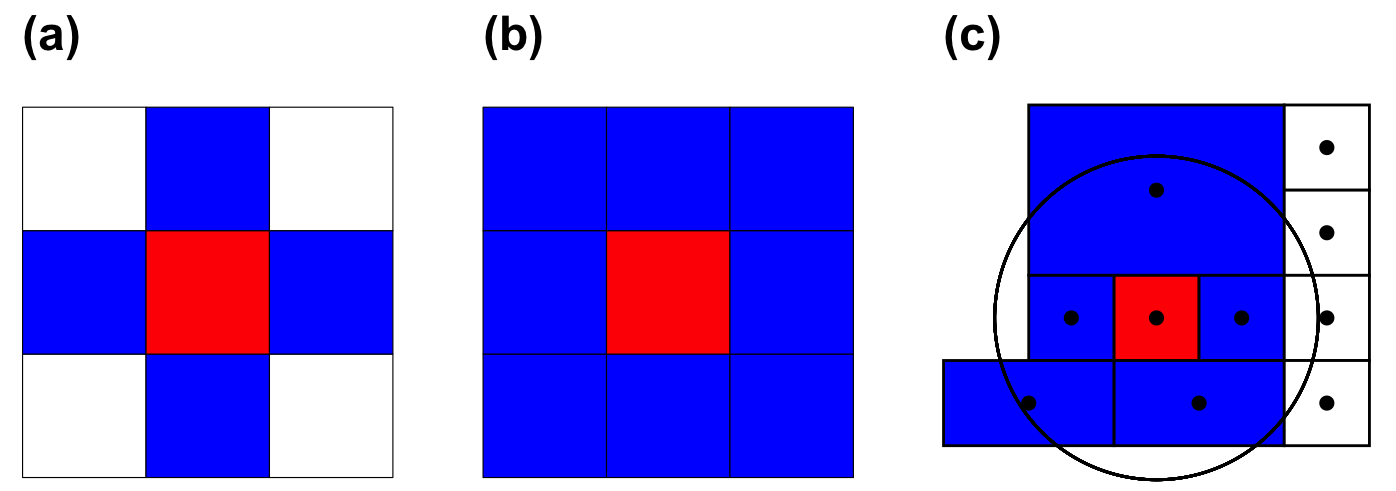
\includegraphics[width=1.0\textwidth]{figures/Neighbors/RookQueen2ndContiguityColored.png}
\caption{(a) Rook neighbors (blue) share an edge with a reference spatial region (red), (b) Queen neighbors (blue) share either an edge or vertex (or both) with a reference spatial region (red), and (c) Distance-based neighbors (blue) have centroids within a fixed radius of the reference cluster (red). Clusters with centroids beyond this distance are not considered as neighbors (white)\cite{moraga_spatial_2024}}
\label{figure:NeighborPlots}
\end{figure}

%DIF <  \begin{figure} [!ht]
%DIF <  \centering
%DIF <  
\includegraphics[width=0.60\textwidth]{figures/Neighbors/RookContiguity.png}
%DIF <  \caption{Rook neighbors (light) share an edge with a reference spatial region (dark)\cite{moraga_spatial_2024}}
%DIF <  \label{figure:RookContiguity}
%DIF <  \end{figure}
\DIFdelbegin %DIFDELCMD < 

%DIFDELCMD < %%%
%DIF <  \begin{figure} [!ht]
%DIF <  \centering
%DIF <  
\includegraphics[width=0.60\textwidth]{figures/Neighbors/QueenContiguity.png}
%DIF <  \caption{Queen neighbors (light) share either an edge or vertex (or both with a reference spatial region (dark)\cite{moraga_spatial_2024}}
%DIF <  \label{figure:QueenContiguity}
%DIF <  \end{figure}
%DIFDELCMD < 

%DIFDELCMD < %%%
%DIF <  Rook & Queen Neighbors
%DIF <  \begin{figure}[!ht]
%DIF <      \centering % Center the entire figure environment
%DIF <      % First Figure (Rook Contiguity)
%DIF <      \begin{minipage}{0.48\textwidth} % Set width to slightly less than half of the text width
%DIF <          \centering % Center the image within its minipage
%DIF <          
\includegraphics[width=\linewidth]{figures/Neighbors/RookContiguityNoTitle.png} % Use \linewidth to fit image to minipage width
%DIF <          \caption{Rook neighbors (light) share an edge with a reference spatial region (dark)\cite{moraga_spatial_2024}}
%DIF <          \label{figure:RookContiguity}
%DIF <      \end{minipage}% <-- **THIS PERCENT SIGN IS CRUCIAL!**
%DIF <      \hfill % \hfill puts a flexible horizontal space between minipages
%DIF <      % Second Figure (Queen Contiguity)
%DIF <      \begin{minipage}{0.48\textwidth} % Set width to slightly less than half of the text width
%DIF <          \centering % Center the image within its minipage
%DIF <          
\includegraphics[width=\linewidth]{figures/Neighbors/QueenContiguityNoTitle.png} % Use \linewidth to fit image to minipage width
%DIF <          \caption{Queen neighbors (light) share either an edge or vertex (or both) with a reference spatial region (dark)\cite{moraga_spatial_2024}}
%DIF <          \label{figure:QueenContiguity}
%DIF <      \end{minipage}
%DIFDELCMD < 

%DIFDELCMD < %%%
%DIF <      % Changed to a regular \caption for a numbered figure, which is more common.
%DIF <      % If you specifically want an unnumbered caption, revert to \caption*{...}.
%DIF <      %\caption{Comparison of Rook and Queen Contiguity Definitions}
%DIF <      %\label{figure:ContiguityComparison} % Overall label for the combined figure
%DIF <  \end{figure}
%DIFDELCMD < 

%DIFDELCMD < %%%
%DIF <  $\textbf{Bishop}$ Neighbors that share a common boundary at the vertex (corners) of the spatial region are known as Bishop neighbors\cite{fotheringham_sage_2009}.
%DIFDELCMD < 

%DIFDELCMD < %%%
%DIF <  $\textbf{Higher-Order Neighbors}$ Spatial regions that do not directly share an edge and/or vertex with another region, but instead share an edge and/or vertex with neighbors of a region are higher-order neighbors. Figure~\ref{figure:HigherOrderNeighbors} illustrates a comparison between the first order neighbors for rook and queen contiguity (top row) versus the second order neighbors for rook and queen contiguity. These higher-order neighbors are ``neighbors of neighbors" of the reference cell.
%DIFDELCMD < 

%DIFDELCMD < %%%
%DIF <  \begin{figure} [!ht]
%DIF <  \centering
%DIF <  
\includegraphics[width=0.70\textwidth]{figures/Neighbors/HigherOrderNeighbors.png}
%DIF <  \caption{Higher order neighbors (light) are ``neighbors of neighbors" of a reference cell (darkest)\cite{moraga_spatial_2024}. Rook neighbors (left) share edge boundaries and Queen neighbors (right) share either edge or vertex boundaries.}
%DIF <  \label{figure:HigherOrderNeighbors}
%DIF <  \end{figure}
%DIFDELCMD < 

%DIFDELCMD < %%%
\DIFdelend \subsubsection{Distance-Based}

%DIF <  SUPP-5: Content moved to Appendix E (R2.1 approved decision)
Distance-based neighbors\cite{fotheringham_sage_2009} identify as neighbors any cluster whose centroid falls within a specified radius of a reference cluster (illustrated in Figure~\ref{figure:NeighborPlots} (c)). A complete description of distance-based neighbor construction and the corresponding spatial weights formulation is provided in Appendix~\ref{appendix:DistanceBased}. The simulation study presented in this paper relies exclusively on Rook contiguity for neighbor definition.

\subsection{Intervention \& Spillover Effects}

Two primary effect types are considered to understand how treatments affect subjects in clusters where they are applied and subjects in the surrounding areas. The intervention effect and spillover effect are two parameters that are estimated in this study. Spatial cluster randomized trials have subjects or regions that are assigned to receive an intervention and others assigned as controls that do not receive an intervention. Observation of the resulting outcomes allows for estimation of the direct intervention effect and indirect spillover effect on the study region.

\subsubsection{Intervention Effect}\label{Section:InterventionEffect}

The intervention effect ($\beta$) \DIFdelbegin \DIFdel{represents the estimated effect of the intervention on clusters that directly receive it}\DIFdelend \DIFaddbegin \DIFadd{is the }\textit{\DIFadd{direct}} \DIFadd{structural coefficient in the spatial autoregressive model of Section~\ref{section:SAR}: the change in a cluster's outcome attributable to its own receipt of the intervention, holding the spillover indicator $z_i$ and the spatial lag fixed}\DIFaddend . Estimation of this \DIFdelbegin \DIFdel{effect }\DIFdelend \DIFaddbegin \DIFadd{coefficient }\DIFaddend is possible due to the presence of clusters assigned as controls for comparison. The relevant intervention could be a vaccine to prevent infectious disease, a training program for government employees, an educational program for students, or many others. \DIFdelbegin \DIFdel{It is worth noting that when spillover propagates }\DIFdelend \DIFaddbegin \DIFadd{We stress that $\beta$ is a structural model coefficient and not a marginal potential-outcome contrast; this distinction is developed formally in the ``Estimands and Interpretation'' paragraph of Section~\ref{section:SAR}. When spillover is permitted to propagate }\DIFaddend back into intervention clusters (\DIFaddbegin \DIFadd{the TrtSpill mechanism; }\DIFaddend see Section~\ref{section:SpilloverEffectTypes}), \DIFdelbegin \DIFdel{the estimated $\hat{\beta}$ may capture elements of both the direct intervention effect and the indirect }\DIFdelend \DIFaddbegin \DIFadd{$\beta$ continues to denote the direct coefficient while the }\DIFaddend spillover received by treated units \DIFdelbegin \DIFdel{; in such scenarios $\hat{\beta}$ is more precisely interpreted as a }\textit{\DIFdel{total treatment effect}} %DIFAUXCMD
\DIFdel{rather than a pure direct effect~}\DIFdelend \DIFaddbegin \DIFadd{is carried by the separate coefficient $\psi$ on $z_i$. If an analyst were instead to fit a model that }\emph{\DIFadd{omits}} \DIFadd{$z_i$, the coefficient on the treatment indicator would conflate the direct and indirect effects through omitted-variable bias---a phenomenon we characterize quantitatively in Section~\ref{section:Results} and Section~\ref{section:Limitations}~}\DIFaddend (R2.M2).

%DIF < %% INTERVENTION EFFECT EQUATION (SIMPLE MODEL) %%%
%DIF <  The response $y$ for subject $i$ considering the intervention effect $\beta$ is expressed as
%DIF <  \begin{equation}
%DIF <      y_i = \alpha + \beta x_i + \varepsilon_i
%DIF <  \end{equation}
%DIF <  where $x_i$ is an indicator of whether subject $i$ receives the intervention, $\alpha$ is a baseline effect, and $\varepsilon_i$ is a random error term for subject $i$.
\DIFdelbegin %DIFDELCMD < 

%DIFDELCMD < %%%
\DIFdelend \subsubsection{Spillover Effect Methods}\label{Section:SpilloverEffectMethods}

The spillover effect ($\psi$) represents an indirect effect on clusters where an intervention was not directly applied\cite{benjamin-chung_spillover_2017}\cite{benjamin-chung_extension_2024}. There are many to model a spillover effect as it is observed due to spatial proximity to subjects or regions where an intervention is applied. In this study, only binary spillover effects were considered. A binary spillover effect is a fixed level of a spillover effect that is applied if a subject or region is deemed to be a neighbor of a subject or region where the intervention is applied. 

%DIF < %% SPILLOVER EFFECT EQUATION (SIMPLE MODEL) %%%
%DIF <  The response for subject $i$ considering this spillover effect is expressed as
%DIF <  \begin{equation}
%DIF <      y_i = \alpha + \beta x_i +\psi z_i + \varepsilon_i.
%DIF <  \end{equation}
%DIF <  where $z_i$ is an indicator of whether the same subject neighbors another subject that receives the intervention and is eligible to experience spillover, $\psi$ is the maximum proportion of the intervention effect that can be experienced as spillover - in this case the binary effect applies 100\% of possible spillover, and $\alpha$, $\beta$, $x_i$, \& $\varepsilon_i$ are as described in Section~\ref{Section:InterventionEffect}. Alternative methods of modeling a spillover effect include: linear, categorical, exponential, and other decay functions\cite{jarvis_spatial_2018}\cite{bian_dual_2025}.
\DIFdelbegin %DIFDELCMD < 

%DIFDELCMD < %%%
%DIF <  but some alternative spillover methods are also discussed. In the following definitions, $x_i$ is an indicator of whether subject $i$ receives the intervention, $z_i$ is an indicator of whether the same subject neighbors another subject that receives the intervention (1) or not (0) and is eligible to experience spillover, $d_{\text{max}}$ is the diameter of each cluster of uniform size, $d_i$ is the distance that a subject is from the nearest intervention source, and $\psi$ is the maximum proportion of the intervention effect that can be experienced as spillover.
%DIFDELCMD < 

%DIFDELCMD < %%%
%DIF <  \begin{itemize}
%DIF <      \item $\textbf{Binary}$: a fixed level of a spillover effect is applied if a subject or region is deemed to be a neighbor of a subject or region where the intervention is applied. This response for subject $i$ considering this spillover effect is expressed as
%DIF <      \begin{equation*}
%DIF <          y_i = \alpha + \beta x_i +\psi z_i + \varepsilon_i.
%DIF <      \end{equation*}
    %DIFDELCMD < 

%DIFDELCMD < %%%
%DIF <      \item $\textbf{Linear}$: The effect of an intervention can decay as distance from the treatment sources increases. A linear decay spillover effect can be applied such that subjects closer to others receiving an intervention experience a greater spillover effect (larger proportion of the intervention effect) and those a greater distance from an intervention source receive a lesser effect (or none) from the intervention. The response for a subject $i$ with a linear decay spillover effect is
%DIF <      \begin{equation*}
%DIF <          y_i = \alpha + \beta x_i + \psi\left(1 - \frac{d_i}{d_{\text{max}}}\right)z_i
%DIF <      \end{equation*}
%DIFDELCMD < 

%DIFDELCMD < %%%
%DIF <      \item $\textbf{Categorical}$: A categorical decay spillover effect models a step-wise drop-off in the proportion of the intervention effect experienced at increasing levels of distance from the nearest intervention source. Contrary to the linear spillover effect, a categorical spillover effect allows for a constant effect to be experienced at concentric bands of distance from an intervention source. Subject $i$ has the following response with consideration of a categorical spillover effect
%DIF <      \begin{align*}
%DIF <          y_i &= \alpha + \beta x_i + \psi\biggl[I\left(d_i \in \left[0, \frac{1}{4}d_{\text{max}}\right]\right)
%DIF <          + 0.75 I\left(d_i \in \left[\frac{1}{4}d_{\text{max}}, \frac{1}{2}d_{\text{max}}\right]\right)\\ &+ 0.50 I\left(d_i \in \left[\frac{1}{2}d_{\text{max}}, \frac{3}{4}d_{\text{max}}\right]\right)
%DIF <          + 0.25 I\left(d_i \in \left[\frac{3}{4}d_{\text{max}}, d_{\text{max}}\right]\right)\biggr]z_i,
%DIF <      \end{align*}
    %DIFDELCMD < 

%DIFDELCMD < %%%
%DIF <      Here, each of the domains of $d_i$ denotes a ``concentric" ring of distance from the intervention zone that receives a certain proportion of the intervention effect (decays in step with distance from the intervention zone). The rings here are the first, second, third, and fourth quartiles of distance from an intervention boundary with respect to the diameter of a cluster.
    %DIFDELCMD < 

%DIFDELCMD < %%%
%DIF <      \item $\textbf{Exponential}$: An exponential decay pattern of spillover has a much ``steeper" drop-off in the effect experienced by a subject neighboring an intervention cluster as the distance from the intervention source increases. This is a reasonable model for spillover if subjects nearby an intervention are expected to experience a strong spillover effect, but subjects that a marginally larger distance and beyond experience little to no effect in the form of spillover. The response for subject $i$ with an exponential decay spillover effect is
%DIF <      \begin{equation*}
%DIF <          y_i = \alpha + \beta x_i + \psi\biggl[\text{exp}\left(-k \frac{d_i}{d_{\text{max}}}\right)\biggr]z_i,
%DIF <      \end{equation*}
%DIFDELCMD < 

%DIFDELCMD < %%%
%DIF <      where $k$ denotes the decay rate of the exponential function.
    %DIFDELCMD < 

%DIFDELCMD < %%%
%DIF <      \item $\textbf{Gaussian}$: A Gaussian decay spillover appears as a ``bell"-shaped distribution when the effect strength is plotted against distance. This decay pattern is similar to exponential decay, but the effect decay is much slower at first before a steep drop-off in effect strength occurs at a moderate to large distance from the intervention source. The response for subject $i$ with a gaussian decay spillover effect (and spread parameter $\sigma$) is
%DIF <      \begin{equation*}
%DIF <          y_i = \alpha + \beta x_i + \psi\text{exp}\left(-\frac{d_{i}^{2}}{2\sigma^2}\right)z_i,
%DIF <      \end{equation*}
%DIFDELCMD < 

%DIFDELCMD < %%%
%DIF <      where small $\sigma$ correspond to a rapid decay of the spillover effect and large $\sigma$ allow for a much larger distance of spillover effect decay.
%DIF <  \end{itemize}
%DIFDELCMD < 

%DIFDELCMD < %%%
\DIFdelend \subsubsection{Spillover Effect Types}\label{section:SpilloverEffectTypes}

In this study, there are two specific ways in which spillover of the applied intervention is allowed to propagate to other cells or subjects. In both cases, spillover effects originate from areas where the original intervention treatment is applied. The first case allows for spillover to propagate from cells receiving the intervention into only cells assigned as control cells. In this case, the effect of the intervention is not permitted to spillover into other intervention cells. This suggests a case where the intervention effect applied is the maximum observable effect and any potential spillover cannot increase the observed effect of a particular intervention. Another method of spillover application is considered where spillover effects are permitted to be applied to both control AND intervention cells that are neighbors of a cell that receives an intervention. This application suggests that an effect greater than that of the original intervention applied can potentially be observed in a cell that received an intervention and also had spillover from another intervention cell. It is also to be expected that any change in the estimated effects would not be observed in spatial settings where the treatment allocation does not satisfy block stratification conditions (where no intervention cells are rook neighbors with other intervention cells). Figure~\ref{figure:TrtNoSpillVsTrtSpill} provides a comparative representation of how these two methods permit the application of spillover effects on clusters based on their treatment assignment. In all scenarios of this simulation study, the application of any spillover effect is simply a binary indication of whether a cluster receives a spillover effect or not. Even if spillover exposure could potentially be directed from multiple neighboring clusters, the modeling in this study does not consider any additive spillover effects.

\begin{figure} [!ht]
\centering

\includegraphics[width=0.80\textwidth]{figures/InterventionSpilloverEffect/TrtSpillComparisonV2.png}
\caption{(a) TrtNoSpill: Spillover arrows flow \emph{outward} from intervention cells (red) into neighboring control cells (blue) only; no spillover enters other intervention cells. (b) TrtSpill: Spillover arrows flow from intervention cells (red) into \emph{both} neighboring control cells (blue) and neighboring intervention cells (red).}
\label{figure:TrtNoSpillVsTrtSpill}
\end{figure}

\subsection{Simple Random vs. Block Stratified Sampling}

In this study, two different treatments are considered: intervention $\&$ control. Assignment of these treatments is considered under two sampling methods: Simple Random Sampling (SRS) $\&$ Block Stratified Sampling (BSS). Random sampling treatment assignment considers all possible combinations of intervention $\&$ control arrangements on a specified spatial grid and provides equal probability of assignment for any given combination of intervention and control. For example, a 2 row by 3 column spatial grid has 6 total cells. Consideration of a 1:1 ratio between intervention and control treatments provides that three cells are assigned as intervention and three cells are assigned as control. Therefore, there are %$\binom{6}{3}=20$ 
$_{6}C_{3}=20$ different combinations of treatments for this specific spatial region. 

Block stratified sampling ensures a balanced number of intervention and control cells are selected, with the added condition that no intervention or control cells share a common edge boundary. This approach is analogous to geographically stratified randomization in standard CRTs, where spatial proximity is used to define strata rather than demographic or clinical covariates\cite{mccann_spatial_2018}\cite{crisp_covariate-constrained_2023}\cite{hayes_cluster_2017}. The added spatial isolation condition---that no two same-treatment clusters may share a Rook edge---is a novel constraint introduced in this work to directly minimize cross-cluster spillover at the design stage. An exception to this rule occurs in spatial setups where both dimensions are odd. In this case, the count of intervention and control cells must be out of balance and we assert that the control class will always be in the majority. In these instances, we relax the common edge boundary restriction for control cells and only require that intervention cells not share a common edge boundary in order to satisfy the block stratification condition.

We now consider a series of spatial grid setups to address efficient estimation of the intervention effect. These spatial grids are have dimensions denoted as (row $\times$ column) and we seek to apply a balanced distribution between intervention and control cells where possible. When this isn't possible, we defer to the control group being the majority class as mentioned previously.

\subsubsection{\DIFdelbegin \DIFdel{2x4 }\DIFdelend Grid \DIFaddbegin \DIFadd{geometries and allocation counts}\DIFaddend }

\DIFdelbegin \DIFdel{One representative spatial setting considered is grid of 8 individual cells laid out in an arrangement of }\DIFdelend \DIFaddbegin \DIFadd{We consider three spatial grid geometries, denoted (row $\times$ column): a }\DIFaddend 2\DIFdelbegin \DIFdel{rows and }\DIFdelend \DIFaddbegin \DIFadd{$\times$}\DIFaddend 4 \DIFdelbegin \DIFdel{columns. For this grid setup, a balanced set of intervention and control cells can be assigned where 4 cells are intervention regions and 4 cells are control regions. For a grid of 8 total cellsand 4 cells of each treatment type, there are %DIF < $\binom{8}{4}=70$
$_{8}C_{4}=70$ unique arrangements of treatment and control assignments. Figure~\ref{figure:GridsCombined} (a)displays one of these combinations that satisfies the block stratified condition where intervention and control cells do not have any rook neighbors of the same treatment type. For this spatial setting, there are 2 (out of 70) combinations that satisfy the block stratification condition. Figure~\ref{figure:GridsCombined} (b) displays an example of the 2x4 grid spatial setting with a randomly sampled arrangement of intervention and control cells. Note that both treatment types have cells that are rook neighbors with the same treatment. These spatial grids are constructed with Simple Features for R package\mbox{%DIFAUXCMD
\cite{pebesma_simple_2018}}\hskip0pt%DIFAUXCMD
\mbox{%DIFAUXCMD
\cite{pebesma_spatial_2023}}\hskip0pt%DIFAUXCMD
.
}%DIFDELCMD < 

%DIFDELCMD < %%%
%DIF <  Figure: Combined Grids (2x4, 3x3, 3x4)
%DIFDELCMD < \begin{figure} [%%%
\DIFdelFL{!ht}%DIFDELCMD < ]
%DIFDELCMD < \centering
%DIFDELCMD < 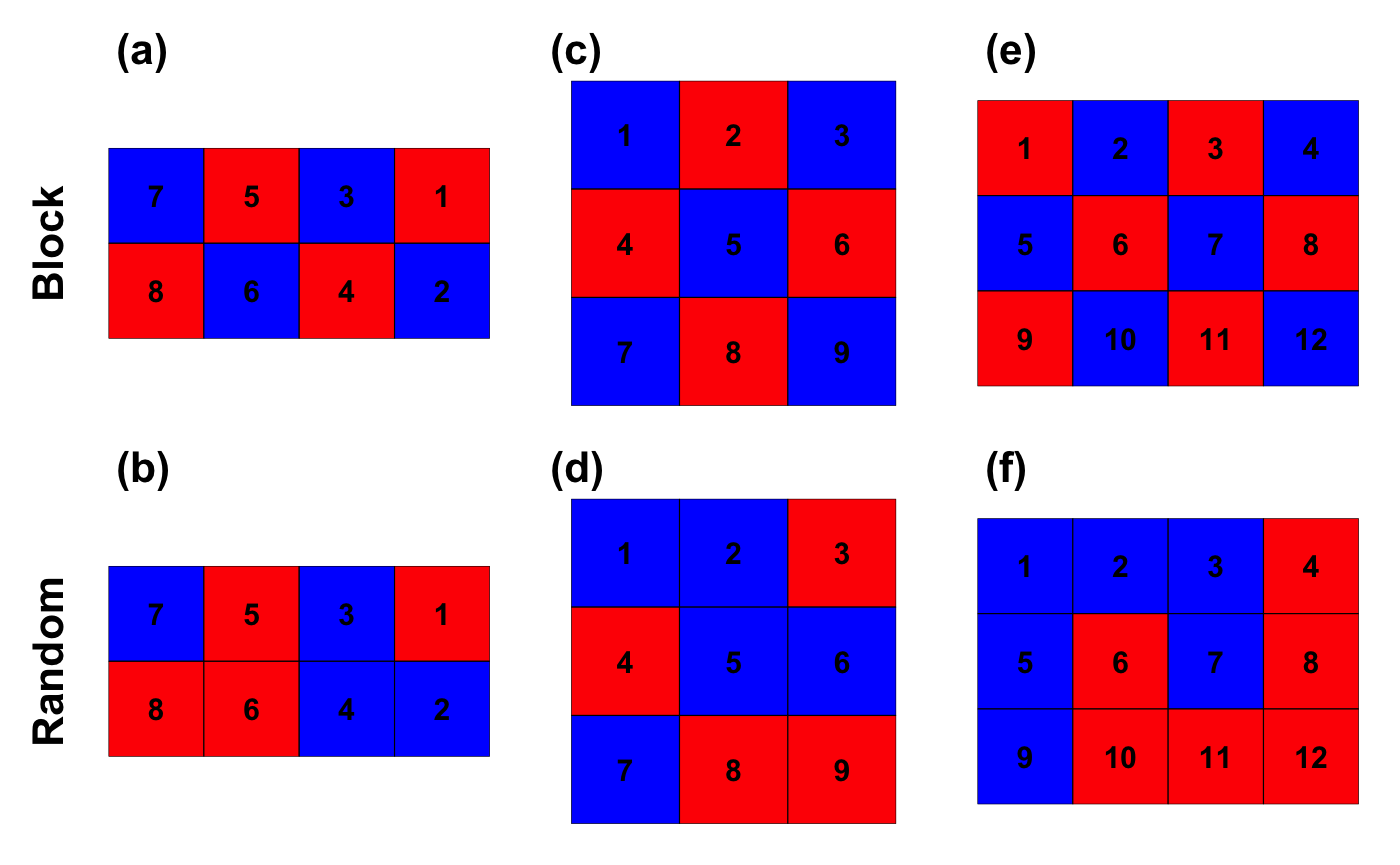
\includegraphics[width=1.0\textwidth]{figures/SpatialGridSetups/GridsCombined.png}
%DIFDELCMD < %%%
%DIFDELCMD < \caption{%
{%DIFAUXCMD
\DIFdelFL{2x4 (left), 3x3 (middle), and 3x4 (right) spatial grids of intervention (red) and control (blue) clusters assigned via Block Stratified Sampling (top row) and Random Sampling (bottom row)}}
%DIFAUXCMD
%DIFDELCMD < \label{figure:GridsCombined}
%DIFDELCMD < \end{figure}
%DIFDELCMD < 

%DIFDELCMD < %%%
%DIF <  2x4 Block & Random Grids
%DIF <  \begin{figure}[!ht]
%DIF <      \centering % Centers the entire block of minipages
%DIFDELCMD < 

%DIFDELCMD < %%%
%DIF <      % Left Column Figure
%DIF <      \begin{minipage}{0.45\textwidth} % Minipage for the left figure
%DIF <          \centering % Centers image within its minipage
%DIF <          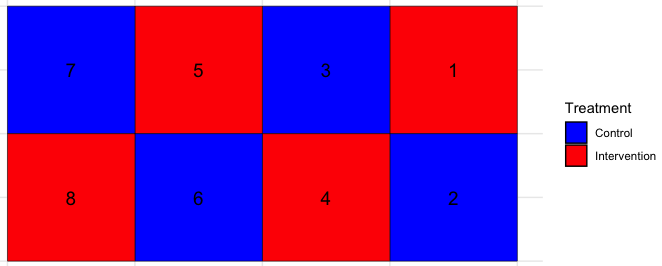
\includegraphics[width=\linewidth]{figures/SpatialGridSetups/Block/BlockStratificationSetup.png}
%DIF <          \caption{2x4 spatial grid of intervention (red) and control (blue) clusters assigned via Block Stratified Sampling}
%DIF <          \label{figure:BlockStratificationSetup}
%DIF <      \end{minipage}%\hspace*{\fill}%  <--- CRITICAL: Ensure NO actual newline character, blank line, or extra spaces between this '%' and the '\begin{minipage}' below. This entire sequence should be one continuous "line" in your .tex file.
%DIF <      \hfill % \hfill puts a flexible horizontal space between minipages
%DIF <      \begin{minipage}{0.45\textwidth} % Minipage for the right figure
%DIF <          \centering % Centers image within its minipage
%DIF <          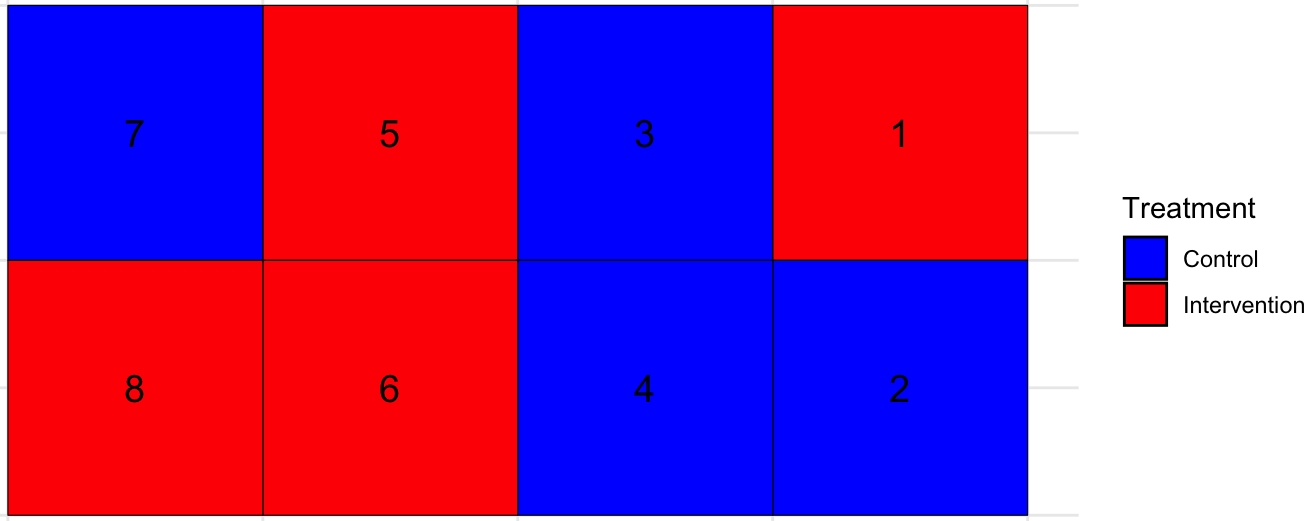
\includegraphics[width=\linewidth]{figures/SpatialGridSetups/Random/RandomSamplingExample2x4.png}
%DIF <          \caption{2x4 spatial grid of intervention (red) and control (blue) clusters assigned via Simple Random Sampling}
%DIF <          \label{figure:RandomSamplingExample2x4}
%DIF <      \end{minipage}
%DIFDELCMD < 

%DIFDELCMD < %%%
%DIF <      % Overall figure caption
%DIF <      %\caption{Comparison of intervention (red) and control (blue) clusters assigned via Block Stratified Sampling (left) and Simple Random Sampling (right) on a 2x4 Grid}
%DIF <      %\label{figure:SamplingComparison2x4}
%DIF <  \end{figure}
%DIFDELCMD < 

%DIFDELCMD < %%%
%DIF < %%%%%%%%%%%%%%%%%%%
%DIFDELCMD < 

%DIFDELCMD < %%%
%DIF <  \begin{figure} [!ht]
%DIF <  \centering
%DIF <  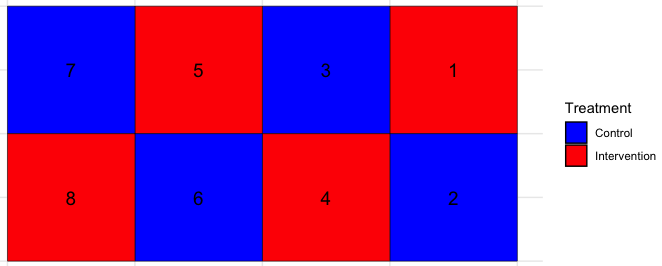
\includegraphics[width=0.70\textwidth]{figures/SpatialGridSetups/Block/BlockStratificationSetup.png}
%DIF <  \caption{2x4 spatial grid of intervention (red) and control (blue) clusters assigned via Block Stratified Sampling}
%DIF <  \label{figure:BlockStratificationSetup}
%DIF <  \end{figure}
%DIFDELCMD < 

%DIFDELCMD < %%%
%DIF <  \begin{figure} [!ht]
%DIF <  \centering
%DIF <  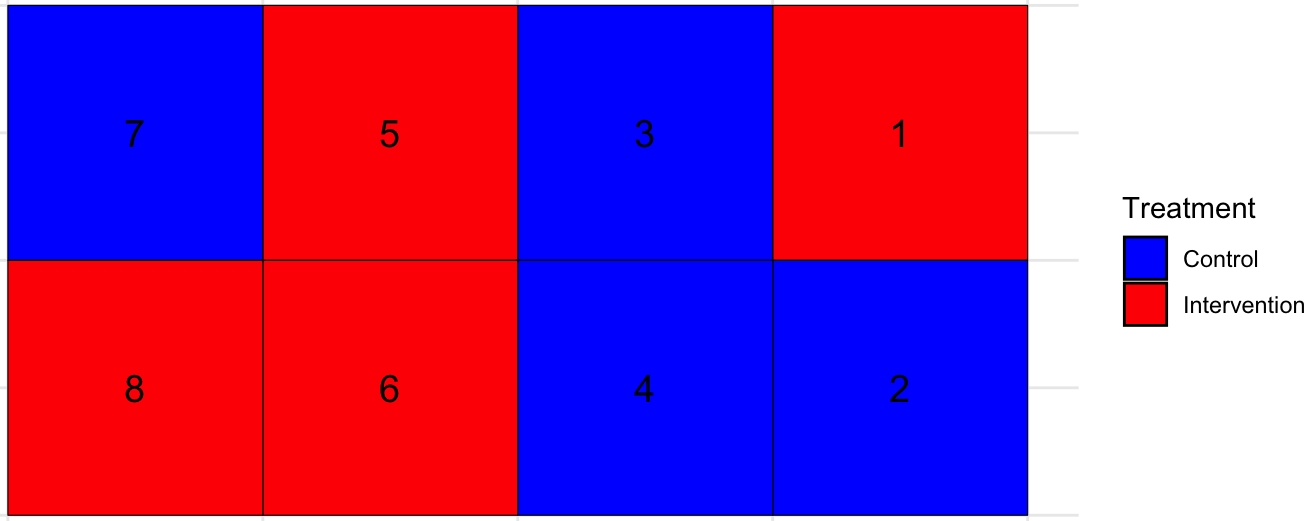
\includegraphics[width=0.70\textwidth]{figures/SpatialGridSetups/Random/RandomSamplingExample2x4.png}
%DIF <  \caption{2x4 spatial grid of intervention (red) and control (blue) clusters assigned via Simple Random Sampling}
%DIF <  \label{figure:RandomSamplingExample2x4}
%DIF <  \end{figure}
%DIFDELCMD < 

%DIFDELCMD < %%%
\subsubsection{\DIFdel{3x3 Grid}}
%DIFAUXCMD
\addtocounter{subsubsection}{-1}%DIFAUXCMD
%DIFDELCMD < 

%DIFDELCMD < %%%
\DIFdel{The 3x3 symmetric }\DIFdelend grid \DIFdelbegin \DIFdel{setting of }\DIFdelend \DIFaddbegin \DIFadd{(8 cells), a symmetric 3$\times$3 grid (}\DIFaddend 9 cells\DIFdelbegin \DIFdel{allows for %DIF < $\binom{9}{4}=\binom{9}{5}=126$ 
$_{9}C_{4}=_{9}C_{5}=126$ unique combinations of intervention and control cells where 5 cells are allocated as control and 4 cells are treatment regions. The majority class of 5 cells is the control group for the sake of hypothetical resource management. Figure~\ref{figure:GridsCombined} (c)illustrates one combination of treatment and control cells that completely satisfies the block stratification conditions. Additional cluster combinations satisfy a relaxed condition of block stratification where control cells are allowed to have other control cells as rook neighbors. This is possible in spatial grid settings where both dimensions (row, column) are odd in length. There is one combination for the 3x3 grid setting that satisfies the strongest block stratification condition and 5 more combinations that satisfy the relaxed block stratification condition for a total of 6. An example of random sampling treatment assignment that doesn't satisfy block stratification conditions is provided in Figure~\ref{figure:GridsCombined} (d).
}%DIFDELCMD < 

%DIFDELCMD < %%%
%DIF <  3x3 Block & Random Grids
%DIF <  \begin{figure}[!ht]
%DIF <      \centering % Centers the entire block of minipages
%DIFDELCMD < 

%DIFDELCMD < %%%
%DIF <      % Left Column Figure
%DIF <      \begin{minipage}{0.45\textwidth} % Minipage for the left figure
%DIF <          \centering % Centers image within its minipage
%DIF <          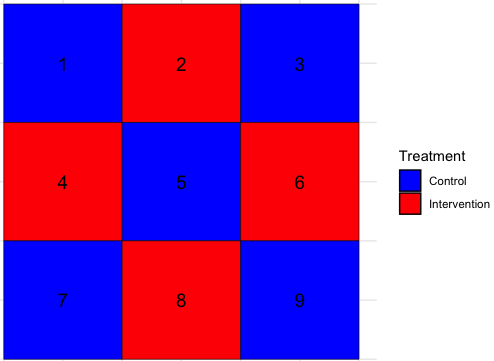
\includegraphics[width=\linewidth]{figures/SpatialGridSetups/Block/BlockStratification3x3.png}
%DIF <          \caption{3x3 spatial grid of clusters with intervention (red) and control (blue) assigned via Block Stratified Sampling}
%DIF <          \label{figure:BlockStratification3x3}
%DIF <      \end{minipage}%\hspace*{\fill}%  <--- CRITICAL: Ensure NO actual newline character, blank line, or extra spaces between this '%' and the '\begin{minipage}' below. This entire sequence should be one continuous "line" in your .tex file.
%DIF <      \hfill % \hfill puts a flexible horizontal space between minipages
%DIF <      \begin{minipage}{0.45\textwidth} % Minipage for the right figure
%DIF <          \centering % Centers image within its minipage
%DIF <          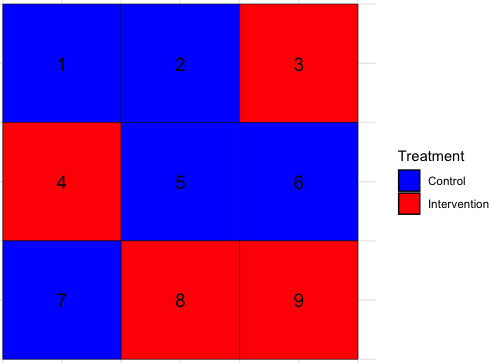
\includegraphics[width=\linewidth]{figures/SpatialGridSetups/Random/RandomSamplingExample3x3.png}
%DIF <          \caption{3x3 spatial grid of intervention (red) and control (blue) clusters assigned via Simple Random Sampling}
%DIF <          \label{figure:RandomSamplingExample3x3}
%DIF <      \end{minipage}
%DIFDELCMD < 

%DIFDELCMD < %%%
%DIF <      % Overall figure caption
%DIF <      % \caption{Comparison of intervention (red) and control (blue) clusters assigned via Block Stratified Sampling (left) and Simple Random Sampling (right) on a 3x3 Grid}
%DIF <      % \label{figure:SamplingComparison3x3}
%DIF <  \end{figure}
%DIFDELCMD < 

%DIFDELCMD < %%%
%DIF < %%%%%%%%%%%%%%%%%%%
%DIFDELCMD < 

%DIFDELCMD < %%%
%DIF <  3x3 Individual Grids
%DIF <  \begin{figure} [!ht]
%DIF <  \centering
%DIF <  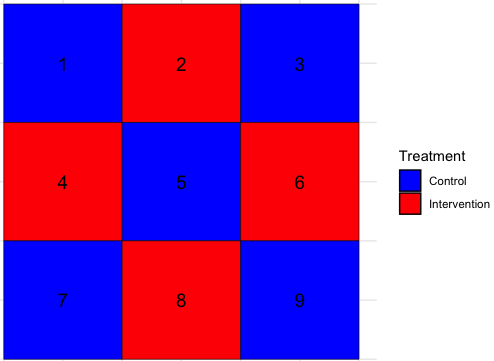
\includegraphics[width=0.70\textwidth]{figures/SpatialGridSetups/Block/BlockStratification3x3.png}
%DIF <  \caption{3x3 spatial grid of clusters with intervention (red) and control (blue) assigned via Block Stratified Sampling}
%DIF <  \label{figure:BlockStratification3x3}
%DIF <  \end{figure}
%DIFDELCMD < 

%DIFDELCMD < %%%
%DIF <  \begin{figure} [!ht]
%DIF <  \centering
%DIF <  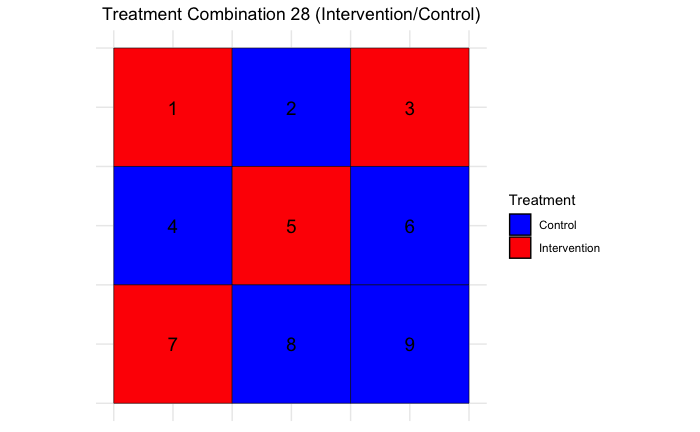
\includegraphics[width=0.70\textwidth]{figures/SpatialGridSetups/Block/BlockStratificationIntSep3x3.png}
%DIF <  \caption{3x3 spatial grid of intervention (red) and control (blue) clusters assigned via relaxed Block Stratified Sampling}
%DIF <  \label{figure:BlockStratificationIntSep3x3}
%DIF <  \end{figure}
%DIFDELCMD < 

%DIFDELCMD < %%%
%DIF <  \begin{figure} [!ht]
%DIF <  \centering
%DIF <  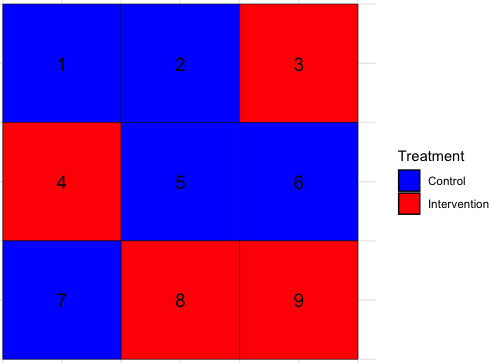
\includegraphics[width=0.70\textwidth]{figures/SpatialGridSetups/Random/RandomSamplingExample3x3.png}
%DIF <  \caption{3x3 spatial grid of intervention (red) and control (blue) clusters assigned via Simple Random Sampling}
%DIF <  \label{figure:RandomSamplingExample3x3}
%DIF <  \end{figure}
%DIFDELCMD < 

%DIFDELCMD < %%%
\subsubsection{\DIFdel{3x4 Grid}}
%DIFAUXCMD
\addtocounter{subsubsection}{-1}%DIFAUXCMD
%DIFDELCMD < 

%DIFDELCMD < %%%
\DIFdel{The final spatial setting considered was a }\DIFdelend \DIFaddbegin \DIFadd{), and a }\DIFaddend 3\DIFdelbegin \DIFdel{row by }\DIFdelend \DIFaddbegin \DIFadd{$\times$}\DIFaddend 4 \DIFdelbegin \DIFdel{column (3x4) grid of }\DIFdelend \DIFaddbegin \DIFadd{grid (}\DIFaddend 12 \DIFdelbegin \DIFdel{total cells. This grid, with a balanced allocation of 6 intervention cells and 6 control cells allows for %DIF < $\binom{12}{6}=924$
$_{12}C_{6}=924$ unique arrangements of the two treatments in the spatial region. For this particular grid size, 2 of the 924 treatment combinations satisfy the block stratification condition and Figure~\ref{figure:GridsCombined} (e)presents one of these, with a ``checkerboard" design. The remaining treatment combinations are achieved via random sampling of a balanced number of intervention and control cells. Figure~\ref{figure:GridsCombined} (f) illustrates another randomly sampled arrangement of the treatments onto the spatial area where control and intervention cells eachhave rook neighbors of the same treatment type.
}%DIFDELCMD < 

%DIFDELCMD < %%%
%DIF <  3x4: Block & Random Grids
%DIF <  \begin{figure}[!ht]
%DIF <      \centering % Centers the entire block of minipages
%DIFDELCMD < 

%DIFDELCMD < %%%
%DIF <      % Left Column Figure
%DIF <      \begin{minipage}{0.45\textwidth} % Minipage for the left figure
%DIF <          \centering % Centers image within its minipage
%DIF <          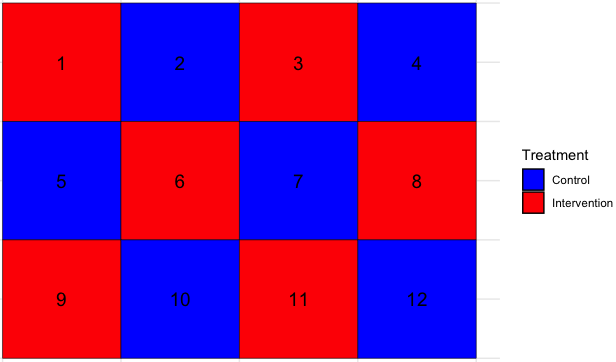
\includegraphics[width=\linewidth]{figures/SpatialGridSetups/Block/BlockStratification3x4.png}
%DIF <          \caption{3x4 spatial grid of clusters with intervention (red) and control (blue) assigned via Block Stratified Sampling}
%DIF <          \label{figure:BlockStratification3x4}
%DIF <      \end{minipage}%\hspace*{\fill}%  <--- CRITICAL: Ensure NO actual newline character, blank line, or extra spaces between this '%' and the '\begin{minipage}' below. This entire sequence should be one continuous "line" in your .tex file.
%DIF <      \hfill % \hfill puts a flexible horizontal space between minipages
%DIF <      \begin{minipage}{0.45\textwidth} % Minipage for the right figure
%DIF <          \centering % Centers image within its minipage
%DIF <          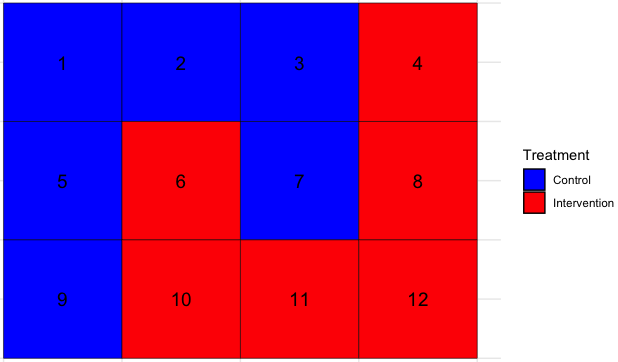
\includegraphics[width=\linewidth]{figures/SpatialGridSetups/Random/RandomSamplingExample3x4.png}
%DIF <          \caption{3x4 spatial grid of intervention (red) and control (blue) clusters assigned via Simple Random Sampling}
%DIF <          \label{figure:RandomSamplingExample3x4}
%DIF <      \end{minipage}
%DIFDELCMD < 

%DIFDELCMD < %%%
%DIF <      % Overall figure caption
%DIF <      % \caption{Comparison of intervention (red) and control (blue) clusters assigned via Block Stratified Sampling (left) and Simple Random Sampling (right) on a 3x4 Grid}
%DIF <      % \label{figure:SamplingComparison3x4}
%DIF <  \end{figure}
%DIFDELCMD < 

%DIFDELCMD < %%%
%DIF < %%%%%%%%%%%%%%%%%%%
%DIFDELCMD < 

%DIFDELCMD < %%%
%DIF <  3x4: Individual Grids
%DIF <  \begin{figure} [!ht]
%DIF <  \centering
%DIF <  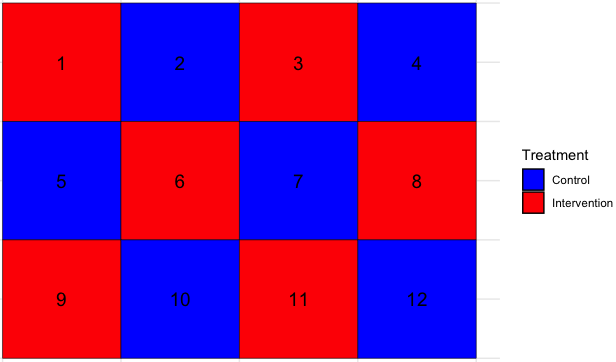
\includegraphics[width=0.70\textwidth]{figures/SpatialGridSetups/Block/BlockStratification3x4.png}
%DIF <  \caption{3x4 spatial grid of clusters with intervention (red) and control (blue) assigned via Block Stratified Sampling}
%DIF <  \label{figure:BlockStratification3x4}
%DIF <  \end{figure}
%DIFDELCMD < 

%DIFDELCMD < %%%
%DIF <  \begin{figure} [!ht]
%DIF <  \centering
%DIF <  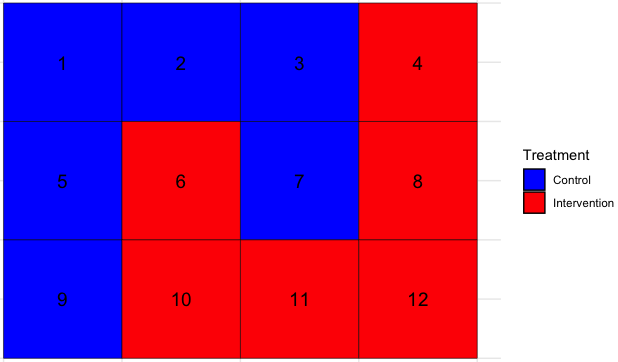
\includegraphics[width=0.70\textwidth]{figures/SpatialGridSetups/Random/RandomSamplingExample3x4.png}
%DIF <  \caption{3x4 spatial grid of intervention (red) and control (blue) clusters assigned via Simple Random Sampling}
%DIF <  \label{figure:RandomSamplingExample3x4}
%DIF <  \end{figure}
%DIFDELCMD < 

%DIFDELCMD < %%%
\subsection{\DIFdel{Spatial Autoregressive (SAR) Model}}%DIFAUXCMD
\addtocounter{subsection}{-1}%DIFAUXCMD
%DIFDELCMD < \label{section:SAR}
%DIFDELCMD < 

%DIFDELCMD < %%%
\DIFdel{Outcomes in the presence of spatial dependence and spillover effects can be considered via modeling with a spatial autoregressive}%DIFDELCMD < \\ %%%
\DIFdel{model\mbox{%DIFAUXCMD
\cite{waller_applied_2004}}\hskip0pt%DIFAUXCMD
\mbox{%DIFAUXCMD
\cite{fotheringham_sage_2009}}\hskip0pt%DIFAUXCMD
\mbox{%DIFAUXCMD
\cite{ullah_handbook_1998}}\hskip0pt%DIFAUXCMD
. A spatial autoregressive model has the form:
}%DIFDELCMD < 

%DIFDELCMD < %%%
\begin{displaymath}\DIFdel{%DIFDELCMD < \label{Equation:SARmodel}%%%
    y_{ik} = \rho\sum_j w_{ij}y_{jk'} + \mathbf{x}_i \beta + \varepsilon_i
}\end{displaymath}%DIFAUXCMD
%DIFDELCMD < 

%DIFDELCMD < \noindent %%%
\DIFdel{where $k$ and $k'$ are different cluster indices for each individual, $\rho$ is the spatial correlation (autoregressive) coefficient, and $\varepsilon_i$ represents an i.i.d. error term. This can also be expressed in matrix notation as:
}%DIFDELCMD < 

%DIFDELCMD < %%%
\begin{displaymath}
    \DIFdel{\mathbf{y} = \rho\mathbf{Wy}+\mathbf{X}\beta + \varepsilon
}\end{displaymath}%DIFAUXCMD
\DIFdel{It follows that the general form of the response for this model for the purpose of this study is
}\begin{displaymath}
    \DIFdel{y_{ik} = \alpha + \beta x_{ik} + \psi z_{ik} + \rho\mathbf{Wy} + \epsilon_i
}\end{displaymath}%DIFAUXCMD
\DIFdel{where $y_i$ is the observed response for subject $i$}\DIFdelend \DIFaddbegin \DIFadd{cells). For each}\DIFaddend , \DIFdelbegin \DIFdel{$\alpha$ is the baseline effect, $\beta$ is the intervention effect, $x_i$ is an indicator of whether subject $i$ receives the intervention, $\psi(d_i)$ is the spillover effect expressed as a function of distance from the nearest intervention source for subject $i$, $z_i$ is an indicator of whether subject $i$ belongs to a cluster that is a Rook neighbor of at least one intervention cluster, making that subject eligible to receive spillover, and $\rho\mathbf{Wy}$ captures spatial dependence from neighboring observations and their effects in the response variable. The components of $\rho\mathbf{Wy}$ are $\rho$, a fixed spatial correlation parameter, $\mathbf{W}$, the spatial weights matrix indicating the strength of relationship between neighboring observations, and the response vector $\mathbf{y}$. Finally, $\varepsilon_i$ is a random error term for each subject.
}%DIFDELCMD < 

%DIFDELCMD < %%%
%DIF <  R1.2: rho vs. psi distinction paragraph
\DIFdel{It is important to clarify the conceptual distinction between two spatial quantities in this model: the spatial autocorrelation parameter $\rho$ and the spillover effect $\psi$. The parameter $\rho$ is a }\emph{\DIFdel{nuisance}} %DIFAUXCMD
\DIFdel{parameter reflecting background spatial correlation in outcomes---nearby clusters tend to produce similar outcomes due to shared environmental, demographic, or social factors, independent of any intervention. In contrast, the spillover effect $\psi$ is a }\emph{\DIFdel{causal, design-level}} %DIFAUXCMD
\DIFdel{quantity representing the indirect effect that an intervention in one cluster exerts on outcomes in neighboring clusters. While both quantities involve spatial proximity, $\rho$ is an intrinsic property of the data-generating process that must be accounted for in order to obtain valid inferences, whereas $\psi$ is of direct scientific interest and often a primary estimand alongside the intervention effect $\beta$. Failure to distinguish these two quantities---or to include both in the model---can produce confounded estimates of the intervention effect. In particular, when spatial dependence is high, failing to include $\rho$ in the model may cause the spillover estimate $\hat{\psi}$ to absorb background correlation, overstating the apparent indirect effect of the intervention.
}%DIFDELCMD < 

%DIFDELCMD < %%%
\subsection{\DIFdel{Spatial Dependence}}%DIFAUXCMD
\addtocounter{subsection}{-1}%DIFAUXCMD
%DIFDELCMD < \label{section:SpatialWeightsMatrix}
%DIFDELCMD < 

%DIFDELCMD < %%%
\DIFdel{Spatial dependence, used interchangeably with spatial autocorrelation, refers to the property of spatial data where observations close to each other tend not be independent of each other. Rather, observations that are close to each other tend to be dependent on each other and influence values of surrounding data. Hence, there is an implied systematic correlation between data at neighboring locations. Spatial correlation can be positive, where similar values tend to be clustered close together, or negative, where dissimilar values are close together. Appropriate consideration of spatial dependence is necessary for performing valid statistical inference as well as for accurate estimation of effects that are modeled. A pair of common methods for assessing spatial autocorrelation are Moran's $\textit{I}$ \mbox{%DIFAUXCMD
\cite{moran_interpretation_1948}}\hskip0pt%DIFAUXCMD
\mbox{%DIFAUXCMD
\cite{moran_notes_1950} }\hskip0pt%DIFAUXCMD
and Geary's $\textit{C}$ \mbox{%DIFAUXCMD
\cite{geary_contiguity_1954}}\hskip0pt%DIFAUXCMD
\mbox{%DIFAUXCMD
\cite{waller_applied_2004}}\hskip0pt%DIFAUXCMD
. Moran's $\textit{I}$ standardizes the spatial auto-covariance by the variance of the data and Geary's $\textit{C}$ utilizes the sum of the squared differences between pairs of data as a measure of co-variation. These test statistics are reliant on the spatial weights matrix. Formal expressions for both statistics are provided in Appendix~D.
}%DIFDELCMD < 

%DIFDELCMD < %%%
%DIF <  \subsubsection{Tests of Spatial Dependence - Moran's \textit{I}}
%DIFDELCMD < 

%DIFDELCMD < %%%
%DIF <  The Moran's $\textit{I}$ statistic quantifies the degree of similarity or dissimilarity between neighboring data using standardized spatial covariance. The statistic takes on values from -1 (negative autocorrelation) to 1 (positive autocorrelation) where the expected value under a null hypothesis of no spatial autocorrelation is $E\left[\textit{I}\right] = -\left(N-1\right)^{-1}$ , where $N$ is the count of spatial units. Moran's $\textit{I}$ has the form
%DIF <  \begin{equation*}
%DIF <      \textit{I} = \frac{N\sum_{i=1}^{N}\sum_{j=1}^{N}w_{ij}\left(x_i - \bar{x}\right)\left(x_j-\bar{x}\right)}{\left(\sum_{i=1}^{N}\sum_{j=1}^{N}w_{ij}\right)\sum_{i=1}^{N}\left(x_i - \bar{x}\right)^2}
%DIF <  \end{equation*}
%DIF <  where
%DIF <  \begin{itemize}
%DIF <      \item $N$ is the number of spatial units
%DIF <      \item $x_i$ is the value of a unit at location $i$
%DIF <      \item $\bar{X}$ is the average of the unit values
%DIF <      \item $w_{ij}$ are elements of the spatial weights matrix.
%DIF <  \end{itemize}
%DIFDELCMD < 

%DIFDELCMD < %%%
%DIF <  Moran's $\textit{I}$ can be implemented with the `moran.test()' function from the spdep package in R\cite{bivand_comparing_2018}.
%DIFDELCMD < 

%DIFDELCMD < %%%
%DIF <  \subsubsection{Tests of Spatial Dependence - Geary's \textit{C}}
%DIFDELCMD < 

%DIFDELCMD < %%%
%DIF <  The Geary's $\textit{C}$ statistic considers the sum of squared differences between adjacent observations or values. Values that are significantly less than 1 are an indication of rising positive spatial autocorrelation and values much higher than 1 represent increasing negative spatial correlation. Under the null hypothesis of no spatial autocorrelation, the expected value is $E\left[\textit{C}\right] = 1$. The applicable formula of the statistic is
%DIF <  \begin{equation*}
%DIF <      \textit{C} = \frac{\left(N-1\right)\sum_{i=1}^{N}\sum_{j=1}^{N} w_{ij}\left(x_i-x_j\right)^2}{2\left(\sum_{i=1}^{N}\sum_{j=1}^{N}w_{ij}\right)\sum_{i=1}^{N}\left(x_i-\bar{x}\right)^2}
%DIF <  \end{equation*}
%DIF <  where
%DIF <  \begin{itemize}
%DIF <      \item $N$ is the number of spatial units
%DIF <      \item $x_i$ and $x_j$ are unit values at locations $i$ and $j$
%DIF <      \item $\bar{x}$ is the average of the unit values
%DIF <      \item $w_{ij}$ are the elements of the spatial weights matrix.
%DIF <  \end{itemize}
%DIFDELCMD < 

%DIFDELCMD < %%%
%DIF <  Geary's $\textit{C}$ can be implemented with the `geary.test()' function from the spdep package in R\cite{bivand_comparing_2018}.
%DIFDELCMD < 

%DIFDELCMD < %%%
%DIF < \subsubsection{Spatial Weights Matrix}
%DIFDELCMD < 

%DIFDELCMD < %%%
%DIF <  SUPP-1: Spatial weights equations moved to Appendix A
\DIFdel{The spatial weights matrix $\mathbf{W}$ encodes the strength of spatial connections between observations; its elements $w_{ij}$ can be constructed as indicator-based (Rook contiguity) or distance-based weights, both of which are row-normalized to ensure comparability across observations with differing numbers of neighbors. In this study, row-normalized indicator (Rook contiguity) weights are used throughout. The spatial dependence term of the SAR model is therefore
}%DIFDELCMD < 

%DIFDELCMD < %%%
\begin{displaymath}\DIFdel{%DIFDELCMD < \label{Equation:SpatialDepTerm}%%%
    \rho\mathbf{Wy} = \rho\sum_{j \in \mathcal{N}(i)}w_{ij}y_j
}\end{displaymath}%DIFAUXCMD
%DIFDELCMD < 

%DIFDELCMD < %%%
\DIFdel{where $\mathcal{N}(i)$ denotes the set of subjects belonging to clusters that are Rook neighbors of the cluster containing subject $i$. Full definitions of indicator-based and distance-based weight construction, including row-normalization formulas, are provided in Appendix~\ref{appendix:SpatialWeights}.
}%DIFDELCMD < 

%DIFDELCMD < %%%
\subsection{\DIFdel{Estimation for SAR Model}}
%DIFAUXCMD
\addtocounter{subsection}{-1}%DIFAUXCMD
%DIFDELCMD < 

%DIFDELCMD < %%%
%DIF <  SUPP-2: Full likelihood/log-likelihood moved to Appendix B
\DIFdel{Maximum likelihood estimation is utilized to gather parameter estimates from the spatial lag model from Section~\ref{section:SAR}\mbox{%DIFAUXCMD
\cite{ord_estimation_1975}}\hskip0pt%DIFAUXCMD
\mbox{%DIFAUXCMD
\cite{bivand_comparing_2015}}\hskip0pt%DIFAUXCMD
\mbox{%DIFAUXCMD
\cite{bivand_computing_2013}}\hskip0pt%DIFAUXCMD
. The subject-level model to be estimated is
}%DIFDELCMD < 

%DIFDELCMD < %%%
\begin{displaymath}\DIFdel{%DIFDELCMD < \label{Equation:SARestimation}%%%
    y_i = \rho \sum_{j\neq i}w_{ij}y_{j} + \alpha + \beta x_i + \psi z_i + \epsilon_i
}\end{displaymath}%DIFAUXCMD
%DIFDELCMD < 

%DIFDELCMD < %%%
\DIFdel{where all terms are as defined in Section~\ref{section:SAR}. The full likelihood and log-likelihood expressions, along with details of the MLE derivation, are provided in Appendix~\ref{appendix:SARLikelihood}. In applied tasks, estimates are obtained via the }\texttt{\DIFdel{lagsarlm()}} %DIFAUXCMD
\DIFdel{function from the }\textbf{\DIFdel{spdep}} %DIFAUXCMD
\DIFdel{R library\mbox{%DIFAUXCMD
\cite{bivand_r_2022}}\hskip0pt%DIFAUXCMD
.
}%DIFDELCMD < 

%DIFDELCMD < %%%
%DIF <  --- SIMULATIONS (application) ---
\section{\DIFdel{Simulation Study}}%DIFAUXCMD
\addtocounter{section}{-1}%DIFAUXCMD
%DIFDELCMD < \label{section:Results}
%DIFDELCMD < 

%DIFDELCMD < %%%
\DIFdel{A simulation study was carried out to consider the contrast of block stratified and random treatment assignment sampling methods with consideration for spillover effects, spatial dependence, and restrictions on spillover application between intervention and control regions. The results of this study are detailed in the remainder of this section.
}%DIFDELCMD < 

%DIFDELCMD < %%%
\subsection{\DIFdel{Simulation Scenarios \& Response}}
%DIFAUXCMD
\addtocounter{subsection}{-1}%DIFAUXCMD
%DIFDELCMD < 

%DIFDELCMD < %%%
\DIFdel{We carry out a simulation study to explore how estimation error of the intervention effect in a Spatial CRT varies across a range of spillover effect sizes, the presence or absence of spatial dependence, varying restrictions on clusters where spillover is permitted to occur, and the method of sampling for treatment assignment. Each simulation scenario is composed of a set of these parameters. The baseline effect, $\alpha$, is always assigned as $0.2$. The intervention effect, $\beta$, is always assigned as $1.0$. The spillover effect, $\psi$, has possible values $0.5$, $0.6$, $0.7$, and $0.8$. The spatial dependence parameter, $\rho$ is set as either $0.00$ }\DIFdelend \DIFaddbegin \DIFadd{simple random sampling (SRS) draws from all balanced (}\DIFaddend or\DIFdelbegin \DIFdel{$0.01$. The sampling design for each scenario is either Block Stratified Sampling (BSS) or Simple Random Sampling (SRS) . Finally, the spillover application type is (1) Control Clusters Only or (2) Control \& Intervention Clusters. Each simulation setting is replicated for each of the spatial grid dimensions discussed previously (2x4}\DIFdelend , \DIFdelbegin \DIFdel{3x3, and 3x4).
}%DIFDELCMD < 

%DIFDELCMD < %%%
\DIFdel{Given that the form of the spatial lag model in Section~\ref{section:SAR} contains the response on both sides of the expression, a separate closed-form expression for data generation must be considered\mbox{%DIFAUXCMD
\cite{fotheringham_sage_2009}}\hskip0pt%DIFAUXCMD
\mbox{%DIFAUXCMD
\cite{baltagi_spatial_2003}}\hskip0pt%DIFAUXCMD
. This data generation expression is
}%DIFDELCMD < 

%DIFDELCMD < %%%
\begin{displaymath}\DIFdel{%DIFDELCMD < \label{Equation:DataGen}%%%
    \mathbf{y} = \left(\mathbf{I}-\rho \mathbf{W}\right)^{-1}\left(\boldsymbol\alpha + \mathbf{X}\boldsymbol\beta + \epsilon\right)
}\end{displaymath}%DIFAUXCMD
\DIFdel{where $X\beta = \beta x_i + \psi z_i$. $x_i$ is an indicator of whether subject $i$ receives the intervention and $z_i$ is an indicator of whether subject $i$ receives any spillover effect.
}%DIFDELCMD < 

%DIFDELCMD < %%%
%DIF <  % --- REMOVE TABLE OF SCENARIOS
%DIF <  \begin{table}[ht!]
%DIF <  \centering
%DIF <  \begin{tabular}{c c c c c c c}
%DIF <      \toprule
%DIF <      \textbf{Index} & \textbf{Alpha} & \textbf{Beta} & \textbf{\makecell{Spillover \\ Effect ($\psi$)}} & \textbf{\makecell{Spatial \\ Dependence ($\rho$)}} & \textbf{\makecell{Sampling \\ Design}} & \textbf{\makecell{Spillover Type}} \\
%DIF <      \midrule
%DIF <      % --- Control Only scenarios (Rows 1-16) ---
%DIF <      \textbf{Scenario 1} & 0.2 & 1.0 & 0.5 & 0.01 & SRS & Control Only \\
%DIF <      \textbf{Scenario 2} & 0.2 & 1.0 & 0.6 & 0.01 & SRS & Control Only \\
%DIF <      \textbf{Scenario 3} & 0.2 & 1.0 & 0.7 & 0.01 & SRS & Control Only \\
%DIF <      \textbf{Scenario 4} & 0.2 & 1.0 & 0.8 & 0.01 & SRS & Control Only \\
%DIF <      \cmidrule(lr){1-7}
%DIF <      \textbf{Scenario 5} & 0.2 & 1.0 & 0.5 & 0.00 & SRS & Control Only \\
%DIF <      \textbf{Scenario 6} & 0.2 & 1.0 & 0.6 & 0.00 & SRS & Control Only \\
%DIF <      \textbf{Scenario 7} & 0.2 & 1.0 & 0.7 & 0.00 & SRS & Control Only \\
%DIF <      \textbf{Scenario 8} & 0.2 & 1.0 & 0.8 & 0.00 & SRS & Control Only \\
%DIF <      \midrule
%DIF <      \textbf{Scenario 9} & 0.2 & 1.0 & 0.5 & 0.01 & BSS & Control Only \\
%DIF <      \textbf{Scenario 10} & 0.2 & 1.0 & 0.6 & 0.01 & BSS & Control Only \\
%DIF <      \textbf{Scenario 11} & 0.2 & 1.0 & 0.7 & 0.01 & BSS & Control Only \\
%DIF <      \textbf{Scenario 12} & 0.2 & 1.0 & 0.8 & 0.01 & BSS & Control Only \\
%DIF <      \cmidrule(lr){1-7}
%DIF <      \textbf{Scenario 13} & 0.2 & 1.0 & 0.5 & 0.00 & BSS & Control Only \\
%DIF <      \textbf{Scenario 14} & 0.2 & 1.0 & 0.6 & 0.00 & BSS & Control Only \\
%DIF <      \textbf{Scenario 15} & 0.2 & 1.0 & 0.7 & 0.00 & BSS & Control Only \\
%DIF <      \textbf{Scenario 16} & 0.2 & 1.0 & 0.8 & 0.00 & BSS & Control Only \\
%DIF <      \midrule
%DIF <      % --- Control & Intervention scenarios (Rows 17-32) ---
%DIF <      \textbf{Scenario 17} & 0.2 & 1.0 & 0.5 & 0.01 & SRS & Control \& Intervention \\
%DIF <      \textbf{Scenario 18} & 0.2 & 1.0 & 0.6 & 0.01 & SRS & Control \& Intervention \\
%DIF <      \textbf{Scenario 19} & 0.2 & 1.0 & 0.7 & 0.01 & SRS & Control \& Intervention \\
%DIF <      \textbf{Scenario 20} & 0.2 & 1.0 & 0.8 & 0.01 & SRS & Control \& Intervention \\
%DIF <      \cmidrule(lr){1-7}
%DIF <      \textbf{Scenario 21} & 0.2 & 1.0 & 0.5 & 0.00 & SRS & Control \& Intervention \\
%DIF <      \textbf{Scenario 22} & 0.2 & 1.0 & 0.6 & 0.00 & SRS & Control \& Intervention \\
%DIF <      \textbf{Scenario 23} & 0.2 & 1.0 & 0.7 & 0.00 & SRS & Control \& Intervention \\
%DIF <      \textbf{Scenario 24} & 0.2 & 1.0 & 0.8 & 0.00 & SRS & Control \& Intervention \\
%DIF <      \midrule
%DIF <      \textbf{Scenario 25} & 0.2 & 1.0 & 0.5 & 0.01 & BSS & Control \& Intervention \\
%DIF <      \textbf{Scenario 26} & 0.2 & 1.0 & 0.6 & 0.01 & BSS & Control \& Intervention \\
%DIF <      \textbf{Scenario 27} & 0.2 & 1.0 & 0.7 & 0.01 & BSS & Control \& Intervention \\
%DIF <      \textbf{Scenario 28} & 0.2 & 1.0 & 0.8 & 0.01 & BSS & Control \& Intervention \\
%DIF <      \cmidrule(lr){1-7}
%DIF <      \textbf{Scenario 29} & 0.2 & 1.0 & 0.5 & 0.00 & BSS & Control \& Intervention \\
%DIF <      \textbf{Scenario 30} & 0.2 & 1.0 & 0.6 & 0.00 & BSS & Control \& Intervention \\
%DIF <      \textbf{Scenario 31} & 0.2 & 1.0 & 0.7 & 0.00 & BSS & Control \& Intervention \\
%DIF <      \textbf{Scenario 32} & 0.2 & 1.0 & 0.8 & 0.00 & BSS & Control \& Intervention \\
%DIF <      \bottomrule
%DIF <  \end{tabular}
%DIF <  \caption{Simulation Scenarios for Intervention Estimation in 2x4, 3x3, and 3x4 Spatial Grid Setting}
%DIF <  \label{table:SimulationSets}
%DIF <  \end{table}
%DIFDELCMD < 

%DIFDELCMD < %%%
%DIF <  R1.3: Inferential scope clarification
\DIFdel{BSS is fundamentally a }\emph{\DIFdel{design-stage}} %DIFAUXCMD
\DIFdel{tool: the set of valid BSS allocations is determined prior to data collection, and this study evaluates estimator behavior by exhaustively enumerating all possible treatment allocations for each spatial grid. This exhaustive enumeration is feasible for the small grids studied here (70, 126, and 924 total combinations, respectively) and directly characterizes the full design space. The simulation does not claim to support permutation-based frequentist inference under BSS, nor does it use BSS as a basis for a randomization distribution. Rather, model-based inference via SAR maximum likelihood estimation---specifically }\DIFdelend \DIFaddbegin \DIFadd{for }\DIFaddend the \DIFdelbegin \texttt{\DIFdel{lagsarlm()}} %DIFAUXCMD
\DIFdel{R function---is the appropriate inferential framework for practitioners implementing either SRS orBSS in an applied study. The role of this simulation is to identify which design choice leads to an estimator with more favorable bias-variance properties when the true data-generating model (SAR with spillover) is correctly specified.
}%DIFDELCMD < 

%DIFDELCMD < %%%
\subsection{\DIFdel{Simulation Procedure}}
%DIFAUXCMD
\addtocounter{subsection}{-1}%DIFAUXCMD
%DIFDELCMD < 

%DIFDELCMD < %%%
\DIFdel{The algorithm implemented to perform the simulations for this study is illustrated in the following section. The simulation is performed over all potential cluster treatment combinations (intervention/control) for each of the 2x4, 3x3, and 3x4 cluster spatial grid geometries. The simulation procedure is as follows:
}%DIFDELCMD < 

%DIFDELCMD < %%%
%DIF <  SUPP-3: Full 8-step procedure moved to Appendix C
\DIFdel{For each spatial grid geometry and simulation scenario, the complete set of possible treatment combinations was enumerated exhaustively (70 for the 2$\times$4 grid, 126 for the }\DIFdelend \DIFaddbegin \DIFadd{odd-dimensioned }\DIFaddend 3$\times$3 grid, \DIFdelbegin \DIFdel{and 924 for the 3$\times$4 grid) . For each combination, $N = 50$ simulation replications were performed for the 2$\times$4 and 3$\times$3 grids and $N = 10$ for the 3$\times$4 grid, with 20 subjects uniformly sampled per cluster in each replication. Outcomes were generated from the SAR closed-form data-generating process (Equation~\ref{Equation:DataGen}), and parameters $(\alpha, \beta, \psi, \rho)$ were estimated via }\texttt{\DIFdel{lagsarlm()}} %DIFAUXCMD
\DIFdel{for each replication. BSS-valid combinations were identified and tracked separately (2 for the 2$\times$4 grid, 6 for 3$\times$3, and 2 for 3$\times$4). The complete step-by-step algorithm, including BSS identification criteria and aggregation procedures, is provided in Appendix~\ref{appendix:SimAlgorithm}.
}%DIFDELCMD < 

%DIFDELCMD < %%%
%DIF <  % --- Refined Algorithm for Simulation Study --- (THIS NEEDS TO BE EDITED)
%DIF <  \begin{algorithm}[ht!]
%DIF <      \caption{[EX: PLACEHOLDER] Simulation Algorithm for Intervention Effect ($\beta$) Estimation}
%DIF <      \label{alg:simulation_framework}
%DIF <      \begin{algorithmic}[1]
%DIF <          \Procedure{Simulate\_Spatial\_RCTs}{$\mathcal{S}, M$}
%DIF <          \Comment{$\mathcal{S}$: Set of all 32 simulation scenarios, $M$: Number of iterations per scenario}
%DIFDELCMD < 

%DIFDELCMD < %%%
%DIF <          \State \textbf{Construct Spatial Objects:}
%DIF <          \State Construct a spatial grid of $N=12$ clusters.
%DIF <          \State Define the spatial weights matrix $W$ based on cluster contiguity (e.g., Queen).
%DIF <          \State Define true parameters: $\beta=1.0$, and the ranges for $\psi$ and $\rho$.
%DIF <          \State Initialize a data structure to store final MSE and SD results for each scenario.
%DIFDELCMD < 

%DIFDELCMD < %%%
%DIF <          \For{each scenario $s$ in the set $\mathcal{S}$}
%DIF <              \Comment{Outer loop iterates through all 32 combinations}
%DIF <              \State Let $s = (\text{Sampling Design}, \rho, \psi, \text{Spillover Type})$.
%DIF <              \State Initialize an empty list $\mathcal{L}_{\hat{\beta}}$ to store estimates from this scenario.
%DIFDELCMD < 

%DIFDELCMD < %%%
%DIF <              \For{iteration $m=1, ..., M$}
%DIF <                  \Comment{Inner loop for Monte Carlo replicates}
%DIF <                  \State \textbf{Assign Treatment and Neighbors:}
%DIF <                  \State Assign $n_I=6$ intervention and $n_C=6$ control clusters based on the \textbf{Sampling Design}.
%DIF <                  \State Identify the set of neighbors for each cluster using the weights matrix $W$.
%DIF <                  \State Define spillover influence according to the \textbf{Spillover Type}.
%DIFDELCMD < 

%DIFDELCMD < %%%
%DIF <                  \State \textbf{Generate Data:}
%DIF <                  \State Generate outcome data $y$ for all clusters from a data generating process that includes:
%DIF <                  \Statex \qquad Spatial dependence (using parameter $\rho$),
%DIF <                  \Statex \qquad Intervention effect (using parameter $\beta$),
%DIF <                  \Statex \qquad Spillover effects (using parameter $\psi$).
%DIF <                  \Statex \qquad Example SAR model: $y = (I - \rho W)^{-1}(X\beta + Z\psi + \epsilon)$.
%DIFDELCMD < 

%DIFDELCMD < %%%
%DIF <                  \State \textbf{Fit Model and Estimate Parameters:}
%DIF <                  \State Fit a Spatial Autoregressive (SAR) model to the generated data.
%DIF <                  \State Estimate the intervention effect parameter $\hat{\beta}^{(m)}$ using Maximum Likelihood Estimation.
%DIF <                  \State Store the estimate: $\mathcal{L}_{\hat{\beta}} \gets \mathcal{L}_{\hat{\beta}} \cup \{\hat{\beta}^{(m)}\}$.
%DIFDELCMD < 

%DIFDELCMD < %%%
%DIF <              \EndFor \Comment{End of iteration loop}
%DIFDELCMD < 

%DIFDELCMD < %%%
%DIF <              \State \textbf{Aggregate Estimates for Scenario:}
%DIF <              \State Aggregate the stored estimates in $\mathcal{L}_{\hat{\beta}}$ across all $M$ iterations.
%DIF <              \State Compute the Mean Squared Error (MSE) and Standard Deviation (SD) for the estimated $\hat{\beta}$.
%DIF <              \State Record these aggregated metrics for scenario $s$.
%DIFDELCMD < 

%DIFDELCMD < %%%
%DIF <          \EndFor \Comment{End of scenario loop}
%DIFDELCMD < 

%DIFDELCMD < %%%
%DIF <          \State \Return Recorded MSE and SD for all scenarios.
%DIF <          \EndProcedure
%DIF <      \end{algorithmic}
%DIF <  \end{algorithm}
%DIFDELCMD < 

%DIFDELCMD < %%%
\DIFdel{Figure~\ref{figure:SampledPoints} presents an example of the 8 cluster 2x4 spatial grid object. 160 subjects (20 subjects for each cluster) with uniformly distributed coordinates are sampled over the area of the spatial object and colored according to their cluster membership. Subject counts are not necessarily identical between any pair of clusters as the sample of subjects is considered over the whole space. Points in any cluster on the grid are subject to the selected treatment (}\DIFdelend \DIFaddbegin \DIFadd{near-balanced) }\DIFaddend intervention/control \DIFdelbegin \DIFdel{) and equally experience any potential spillover along with all other points that are members of that same cluster. Similar illustrative figures of the sampled observations over the spatial grid could be constructed and displayed for the other spatial geometries under consideration in the simulation study.
}%DIFDELCMD < 

%DIFDELCMD < \begin{figure} [%%%
\DIFdelFL{!ht}%DIFDELCMD < ]
%DIFDELCMD < \centering
%DIFDELCMD < 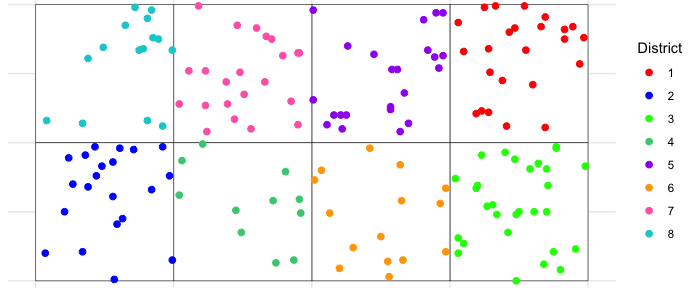
\includegraphics[width=0.80\textwidth]{figures/SpatialGridSetups/SampledPoints.png}
%DIFDELCMD < %%%
%DIFDELCMD < \caption{%
{%DIFAUXCMD
\DIFdelFL{Example of simulated observation coordinates (n=160) on a 2x4 grid of clusters}}
%DIFAUXCMD
%DIFDELCMD < \label{figure:SampledPoints}
%DIFDELCMD < \end{figure}
%DIFDELCMD < 

%DIFDELCMD < %%%
\subsection{\DIFdel{Simulation Evaluation Metrics}}
%DIFAUXCMD
\addtocounter{subsection}{-1}%DIFAUXCMD
%DIFDELCMD < 

%DIFDELCMD < %%%
\DIFdel{Estimates for the baseline effect ($\alpha$), intervention effect ($\beta$), spillover effect ($\psi$), and spatial correlation parameter ($\rho$) were collected for each iteration of the simulation procedure for every treatment assignment combination. Considering the initial fixed simulation parameters, the following metrics are computed for estimation of the intervention effect for the evaluation of each set of simulation conditions.}%DIFDELCMD < \\
%DIFDELCMD < 

%DIFDELCMD < %%%
%DIF <  \begin{itemize}
%DIF <      \item $\textbf{Bias}$: a measure of how different the estimated parameter value is from the true parameter value. Small bias means that the parameter estimate is quite close to the true value.
%DIF <      \item $\textbf{Variance}$: a measure of the spread of a set of estimates from multiple simulation iterations. Smaller variance indicates that the estimates are tightly grouped together and large variance means that the estimates are spread out 
%DIF <      \item $\textbf{Mean Squared Error (MSE)}$: measures the average squared difference between each estimate and the true value of a parameter. Mean Squared Error combines variance to understand the consistency of a set of estimates as well as bias to understand any trend in deviation from the true value into a measure of estimation accuracy.
%DIF <  \end{itemize}
%DIFDELCMD < 

%DIFDELCMD < \noindent %%%
\DIFdel{$\textbf{Bias}$: a measure of how different the estimated parameter value is from the true parameter value. Small bias means that the parameter estimate is quite close to the true value.}%DIFDELCMD < \\
%DIFDELCMD < 

%DIFDELCMD < \noindent %%%
\DIFdel{$\textbf{Variance}$: a measure of the spread of a set of estimates from multiple simulation iterations. Smaller variance indicates that the estimates are tightly grouped together and large variance means that the estimates are spread out.}%DIFDELCMD < \\
%DIFDELCMD < 

%DIFDELCMD < \noindent %%%
\DIFdel{$\textbf{Mean Squared Error (MSE)}$: measures the average squared difference between each estimate and the true value of a parameter. Mean Squared Error combines variance to understand the consistency of a set of estimates as well as bias to understand any trend in deviation from the true value into a measure of estimation accuracy.}%DIFDELCMD < \\
%DIFDELCMD < 

%DIFDELCMD < %%%
%DIF <  R2.5: MSE decomposition / visual representation note
\DIFdel{Since $\text{MSE} = \text{Bias}^2 + \text{Variance}$, differences in MSE between SRS and BSS can be attributed to either systematic bias or sampling variability across allocations. This decomposition is visually reflected in the grouped bar figures throughout the Results section (Figures~\ref{figure:BetaMSE2x4Grouped}--\ref{figure:BetaMSE3x4Grouped}), where the relative contribution of bias-driven versus variance-driven error is apparent from differences in bar height across sampling methods and conditions.
}%DIFDELCMD < 

%DIFDELCMD < %%%
\DIFdel{Mean Squared Error is the primary metric of consideration to understand the efficient estimation of the intervention effect under all simulation settings. The following subsections detail the findings from the simulation study, focusing on the Mean Squared Error (MSE), standard deviation (SD), and bias of the intervention effect ($\beta$) estimates under various conditions (simulation scenarios). The analysis compares Simple Random Sampling (SRS) and Block Stratified Sampling (BSS) across different spatial grid configurations, spillover effect magnitudes, spatial dependence levels, and spillover application types.
}%DIFDELCMD < 

%DIFDELCMD < %%%
\subsection{\DIFdel{Intervention Effect Estimates (2x4 grid)}}
%DIFAUXCMD
\addtocounter{subsection}{-1}%DIFAUXCMD
%DIFDELCMD < 

%DIFDELCMD < %%%
%DIF <  R1.5: Risk-management framing (2x4 grid)
\DIFdel{For the 2$\times$4 spatial grid, the simulation results (Table~1, Figure~\ref{figure:BetaMSE2x4Grouped}) reveal a risk-management trade-off between SRS and BSS rather than a uniform advantage for either method.
}%DIFDELCMD < 

%DIFDELCMD < %%%
\DIFdel{Under the Control Clusters Only (TrtNoSpill) spillover condition, performance depends on the level of spatial dependence. When spatial dependence is present ($\rho = 0.01$), BSS substantially outperforms SRS (e.g., BSS MSE $= 0.165$ vs. SRS MSE $= 0.304$ at $\psi = 0.5$). However, when spatial dependence is absent ($\rho = 0$), SRS achieves lower average MSE (e.g., SRS MSE $= 0.173$ vs. BSS MSE $= 0.262$ at $\psi = 0.5$). Crucially, the standard deviation (SD) of BSS estimates is consistently far smaller than that of SRS across all conditions under TrtNoSpill. This reflects the fact that the two BSS allocations for this grid are structurally similar, yielding reliably consistent estimation error, while the 70 SRS allocations span a wide range of spatial configurations---some well-balanced, some poorly concentrated---producing highly variable MSE.
}%DIFDELCMD < 

%DIFDELCMD < %%%
\DIFdel{Under the Intervention \& Control Clusters (TrtSpill) spillover condition, SRS achieves lower average MSE in every scenario (e.g., SRS MSE $= 0.008$ vs. BSS MSE $= 0.262$ at $\psi = 0.5$, $\rho = 0$). However, the SD of SRS estimates is substantially larger, meaning that while the average SRS allocation performs better, some randomly drawn allocations carry considerable estimation risk. BSS delivers stable---though higher---average MSE with near-zero SD, ensuring that practitioners never encounter a catastrophically poor allocation.
}%DIFDELCMD < 

%DIFDELCMD < %%%
\DIFdel{The presence of spatial dependence ($\rho = 0.01$) consistently increased MSE for both methods relative to the no-dependence setting, a pattern that persists across all grid sizes. The central message from the 2$\times$4 results is that BSS bounds the worst-case outcome at the cost of a somewhat higher average MSE in certain spillover regimes, whereas SRS offers the possibility of a lower average MSE but with substantially greater risk of a high-MSE realization.
}%DIFDELCMD < 

%DIFDELCMD < %%%
%DIF <  --- Figure: Beta MSE for 2x4 (side by side) ---
%DIF <  \begin{figure}[!ht]
%DIF <      \centering % Centers the entire block of minipages
%DIFDELCMD < 

%DIFDELCMD < %%%
%DIF <      % Left Column Figure
%DIF <      \begin{minipage}{0.45\textwidth} % Minipage for the left figure
%DIF <          \centering % Centers image within its minipage
%DIF <          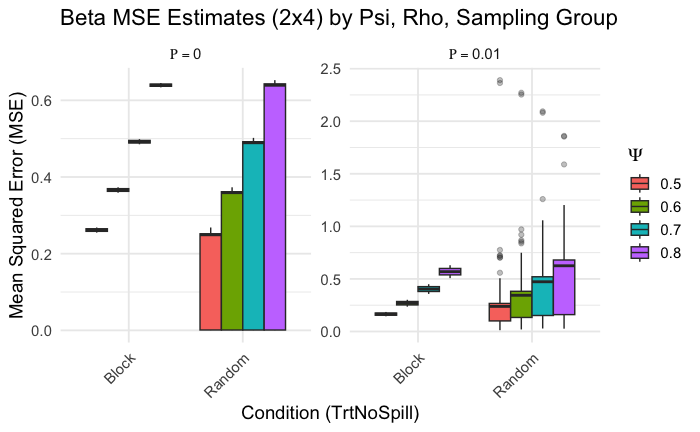
\includegraphics[width=\linewidth]{figures/BetaMSEresults/BetaMSEtrtNoSpill2x4.png}
%DIF <          % \caption{Intervention effect MSE for 2x4 cluster grid with spillover allowed only on control clusters}
%DIF <          % \label{figure:BetaMSEtrtNoSpill2x4}
%DIF <      \end{minipage}%\hspace*{\fill}%  <--- CRITICAL: Ensure NO actual newline character, blank line, or extra spaces between this '%' and the '\begin{minipage}' below. This entire sequence should be one continuous "line" in your .tex file.
%DIF <      \hfill % \hfill puts a flexible horizontal space between minipages
%DIF <      \begin{minipage}{0.45\textwidth} % Minipage for the right figure
%DIF <          \centering % Centers image within its minipage
%DIF <          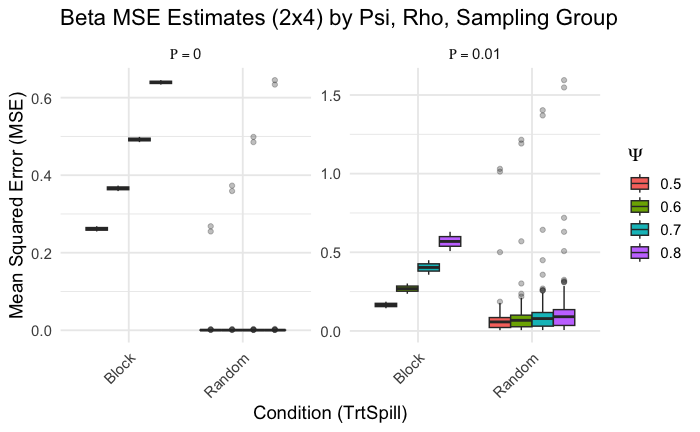
\includegraphics[width=\linewidth]{figures/BetaMSEresults/BetaMSEtrtSpill2x4.png}
%DIF <          % \caption{3x4 spatial grid of intervention (red) and control (blue) clusters assigned via Simple Random Sampling}
%DIF <          % \label{figure:BetaMSEtrtSpill2x4}
%DIF <      \end{minipage}
%DIFDELCMD < 

%DIFDELCMD < %%%
%DIF <      % Overall figure caption
%DIF <      \caption{Intervention effect MSE for 2x4 cluster grid with spillover allowed on control and intervention clusters}
%DIF <      \label{figure:BetaMSE2x4}
%DIF <  \end{figure}
%DIFDELCMD < 

%DIFDELCMD < %%%
%DIF <  --- Figure: Consolidated Intervention MSE for 2x4 grid ---
%DIFDELCMD < \begin{figure} [%%%
\DIFdelFL{!ht}%DIFDELCMD < ]
%DIFDELCMD < \centering
%DIFDELCMD < 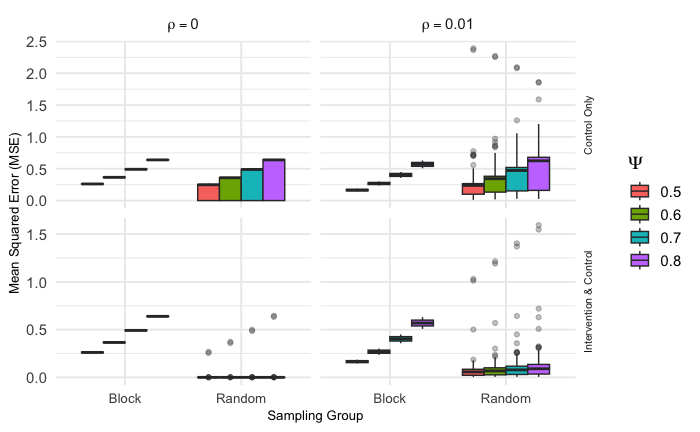
\includegraphics[width=0.80\textwidth]{figures/BetaMSEresults/MSE_Estimates_2x4.png}
%DIFDELCMD < %%%
%DIFDELCMD < \caption{%
{%DIFAUXCMD
\DIFdelFL{Intervention effect MSE for 2x4 cluster grid grouped by spillover effect magnitude, spatial dependence, sampling design, and spillover application type}}
%DIFAUXCMD
%DIFDELCMD < \label{figure:BetaMSE2x4Grouped}
%DIFDELCMD < \end{figure}
%DIFDELCMD < 

%DIFDELCMD < %%%
%DIF <  --- Table: Results for 2x4 Grid ---
%DIF <  \begin{table}[ht!]
%DIF <  \centering % Use \centering for better vertical spacing
%DIF <  \begin{tabular}{ l c c ccc ccc } % 'l' for left-aligned, 'c' for center-aligned
%DIF <      \toprule % Top rule from booktabs package
%DIF <      \textbf{\makecell{Spillover \\ Application}} & \textbf{\makecell{Spatial \\ Dependence \\ ($\rho$)}} & \textbf{\makecell{Spillover \\ Effect \\ ($\psi$)}} & \multicolumn{3}{c}{\textbf{\makecell{Simple Random\\ Sampling}}} & \multicolumn{3}{c}{\textbf{\makecell{Block Stratified\\ Sampling}}} \\
%DIF <      \cmidrule(lr){4-6} \cmidrule(lr){7-9} % Partial rules for sub-headers
%DIF <      & & & MSE & SD & Bias & MSE & SD & Bias \\
%DIF <      \midrule % Mid rule from booktabs package
%DIF <      \multirow{8}{*}{\makecell{Control Only\\ Spillover}} & \multirow{4}{*}{\makecell{Yes ($0.01$)}} & 0.5 & 0.30384 & 0.40525 & -0.26984 & 0.16515 & 0.02943 & -0.34903 \\
%DIF <      & & 0.6 & 0.38161 & 0.40623 & -0.34198 & 0.26900 & 0.04620 & -0.47130 \\
%DIF <      & & 0.7 & 0.47105 & 0.41430 & -0.41415 & 0.40359 & 0.06531 & -0.59377 \\
%DIF <      & & 0.8 & 0.57345 & 0.43896 & -0.48647 & 0.56900 & 0.08672 & -0.71637 \\
%DIF <      \cmidrule(lr){2-9} % Horizontal line spanning from Spatial Dependence to the end
%DIF <      & \multirow{4}{*}{\makecell{No ($0.00$)}} & 0.5 & 0.17278 & 0.11696 & -0.34278 & 0.26160 & 0.00946 & -0.49594 \\
%DIF <      & & 0.6 & 0.24823 & 0.16834 & -0.41130 & 0.36608 & 0.00998 & -0.59661 \\
%DIF <      & & 0.7 & 0.33754 & 0.22914 & -0.47979 & 0.49203 & 0.00951 & -0.69728 \\
%DIF <      & & 0.8 & 0.44075 & 0.29940 & -0.54826 & 0.63946 & 0.00806 & -0.79795 \\
%DIF <      \midrule % Mid rule to separate spillover applications
%DIF <      \multirow{8}{*}{\makecell{Intervention \&\\ Control Spillover}} & \multirow{4}{*}{\makecell{Yes ($0.01$)}} & 0.5 & 0.09543 & 0.17615 & 0.03072 & 0.16515 & 0.02943 & -0.34903 \\
%DIF <      & & 0.6 & 0.11542 & 0.20822 & 0.02984 & 0.26900 & 0.04620 & -0.47130 \\
%DIF <      & & 0.7 & 0.13772 & 0.24225 & 0.02862 & 0.40359 & 0.06531 & -0.59377 \\
%DIF <      & & 0.8 & 0.16216 & 0.27871 & 0.02714 & 0.56900 & 0.08672 & -0.71637 \\
%DIF <      \cmidrule(lr){2-9}
%DIF <      & \multirow{4}{*}{\makecell{No ($0.00$)}} & 0.5 & 0.00790 & 0.04384 & -0.01400 & 0.26160 & 0.00946 & -0.49594 \\
%DIF <      & & 0.6 & 0.01090 & 0.06137 & -0.01679 & 0.36608 & 0.00998 & -0.59661 \\
%DIF <      & & 0.7 & 0.01450 & 0.08250 & -0.01964 & 0.49203 & 0.00951 & -0.69728 \\
%DIF <      & & 0.8 & 0.01872 & 0.10723 & -0.02255 & 0.63946 & 0.00806 & -0.79795 \\
%DIF <      \bottomrule % Bottom rule from booktabs package
%DIF <  \end{tabular}
%DIF <  \caption{SRS vs. BSS: Intervention Effect Error Estimates - 2x4 Spatial Grid Setting}
%DIF <  \label{table:InterventionEstimates2x4}
%DIF <  \end{table}
%DIFDELCMD < 

%DIFDELCMD < \begin{table}[ht!]
%DIFDELCMD < \centering
%DIFDELCMD < \begin{tabular}{l c c ccc ccc}
%DIFDELCMD <     \toprule
%DIFDELCMD <     \textbf{\makecell{Spillover \\ Application}} & \textbf{\makecell{Spatial \\ Dependence \\ ($\rho$)}} & \textbf{\makecell{Spillover \\ Effect \\ ($\psi$)}} & \multicolumn{3}{c}{\textbf{\makecell{Simple Random\\ Sampling}}} & \multicolumn{3}{c}{\textbf{\makecell{Block Stratified\\ Sampling}}} \\
%DIFDELCMD <     \cmidrule(lr){4-6} \cmidrule(lr){7-9}
%DIFDELCMD <     & & & MSE & \makecell{SD \\ ($\times 10$)} & Bias & MSE & \makecell{SD \\ ($\times 10$)} & Bias \\
%DIFDELCMD <     \midrule
%DIFDELCMD <     \multirow{8}{*}{\makecell{Control Only\\ Spillover}} & \multirow{4}{*}{\makecell{Yes ($0.01$)}} & 0.5 & 0.304 & 4.053 & -0.270 & 0.165 & 0.294 & -0.349 \\
%DIFDELCMD <     & & 0.6 & 0.382 & 4.062 & -0.342 & 0.269 & 0.462 & -0.471 \\
%DIFDELCMD <     & & 0.7 & 0.471 & 4.143 & -0.414 & 0.404 & 0.653 & -0.594 \\
%DIFDELCMD <     & & 0.8 & 0.573 & 4.390 & -0.486 & 0.569 & 0.867 & -0.716 \\
%DIFDELCMD <     \cmidrule(lr){2-9}
%DIFDELCMD <     & \multirow{4}{*}{\makecell{No ($0$)}} & 0.5 & 0.173 & 1.170 & -0.343 & 0.262 & 0.095 & -0.496 \\
%DIFDELCMD <     & & 0.6 & 0.248 & 1.683 & -0.411 & 0.366 & 0.100 & -0.597 \\
%DIFDELCMD <     & & 0.7 & 0.338 & 2.291 & -0.480 & 0.492 & 0.095 & -0.697 \\
%DIFDELCMD <     & & 0.8 & 0.441 & 2.994 & -0.548 & 0.639 & 0.081 & -0.798 \\
%DIFDELCMD <     \midrule
%DIFDELCMD <     \multirow{8}{*}{\makecell{Intervention \&\\ Control Spillover}} & \multirow{4}{*}{\makecell{Yes ($0.01$)}} & 0.5 & 0.095 & 1.762 & 0.031 & 0.165 & 0.294 & -0.349 \\
%DIFDELCMD <     & & 0.6 & 0.115 & 2.082 & 0.030 & 0.269 & 0.462 & -0.471 \\
%DIFDELCMD <     & & 0.7 & 0.138 & 2.423 & 0.029 & 0.404 & 0.653 & -0.594 \\
%DIFDELCMD <     & & 0.8 & 0.162 & 2.787 & 0.027 & 0.569 & 0.867 & -0.716 \\
%DIFDELCMD <     \cmidrule(lr){2-9}
%DIFDELCMD <     & \multirow{4}{*}{\makecell{No ($0$)}} & 0.5 & 0.008 & 0.438 & -0.014 & 0.262 & 0.095 & -0.496 \\
%DIFDELCMD <     & & 0.6 & 0.011 & 0.614 & -0.017 & 0.366 & 0.100 & -0.597 \\
%DIFDELCMD <     & & 0.7 & 0.015 & 0.825 & -0.020 & 0.492 & 0.095 & -0.697 \\
%DIFDELCMD <     & & 0.8 & 0.019 & 1.072 & -0.023 & 0.639 & 0.081 & -0.798 \\
%DIFDELCMD <     \bottomrule
%DIFDELCMD < \end{tabular}
%DIFDELCMD < %%%
%DIFDELCMD < \caption{%
{%DIFAUXCMD
\DIFdelFL{SRS vs. BSS: Intervention Effect Error Estimates - 2x4 Spatial Grid Setting}}
%DIFAUXCMD
%DIFDELCMD < \label{table:InterventionEstimates2x4}
%DIFDELCMD < \end{table}
%DIFDELCMD < 

%DIFDELCMD < %%%
%DIF <  \pagebreak
%DIFDELCMD < 

%DIFDELCMD < %%%
\subsection{\DIFdel{Intervention Effect Estimates (3x3 grid)}}
%DIFAUXCMD
\addtocounter{subsection}{-1}%DIFAUXCMD
%DIFDELCMD < 

%DIFDELCMD < %%%
\DIFdel{The results for the 3×3 spatial grid are summarized in Table~2 and Figure~\ref{figure:BetaMSE3x3Grouped}.
}%DIFDELCMD < 

%DIFDELCMD < %%%
\DIFdel{For the Control Clusters Only (TrtNoSpill) spillover application, BSS consistently yielded significantly lower MSE, SD, and bias compared to SRS. For instance, with $\rho=0$, BSS MSE was minimal (e.g., $0.001$ for $\psi=0.5$), while SRS MSE ranged from $0.092$ to $0.235$. This pattern held true with spatial dependence ($\rho=0.01$), where BSS MSE remained very low (e.g., $0.004$ for $\psi=0.5$), contrasting with SRS MSE values ranging from $0.259$ to $0.372$. SRS estimates consistently showed negative bias, increasing with $\psi$, while BSS bias was negligible.
}%DIFDELCMD < 

%DIFDELCMD < %%%
\DIFdel{In the Intervention \& Control Clusters (TrtSpill) spillover scenario, BSS continued to demonstrate superior performance with substantially lower MSE, SD, and bias compared to SRS. For $\rho=0$, BSS MSE was consistently around $0.0004$, whereas SRS MSE ranged from $0.002$ to $0.005$. With $\rho=0.01$, BSS MSE was also consistently very low (e.g., $0.039$ for $\psi=0.5$), while SRS MSE ranged from $0.103$ to $0.168$}\DIFdelend \DIFaddbegin \DIFadd{arrangements, whereas block stratified sampling (BSS) retains only those arrangements satisfying the spatial isolation condition}\DIFaddend . \DIFdelbegin %DIFDELCMD < 

%DIFDELCMD < %%%
\DIFdel{Similar to the 2×4 grid, the presence of spatial dependence ($\rho=0.01$) generally increased MSE for both sampling methods across both spillover application types for the 3×3 grid.
}%DIFDELCMD < 

%DIFDELCMD < %%%
%DIF <  --- Figure: Beta MSE for 3x3 (side by side) ---
%DIF <  \begin{figure}[!ht]
%DIF <      \centering % Centers the entire block of minipages
%DIFDELCMD < 

%DIFDELCMD < %%%
%DIF <      % Left Column Figure
%DIF <      \begin{minipage}{0.45\textwidth} % Minipage for the left figure
%DIF <          \centering % Centers image within its minipage
%DIF <          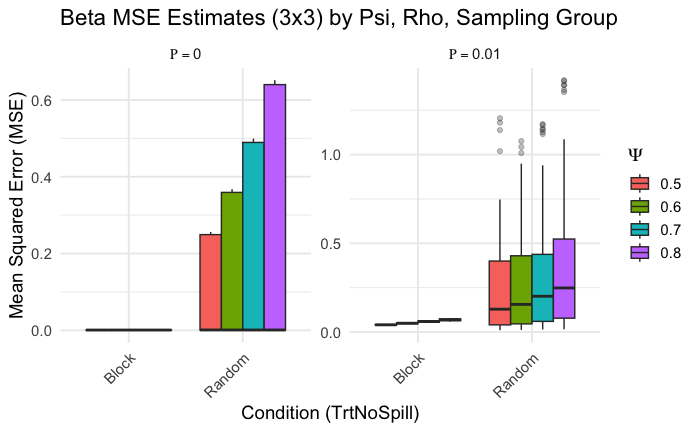
\includegraphics[width=\linewidth]{figures/BetaMSEresults/BetaMSEtrtNoSpill3x3.png}
%DIF <          % \caption{Intervention effect MSE for 3x3 cluster grid with spillover allowed only on control clusters}
%DIF <          % \label{figure:BetaMSEtrtNoSpill3x3}
%DIF <      \end{minipage}%\hspace*{\fill}%  <--- CRITICAL: Ensure NO actual newline character, blank line, or extra spaces between this '%' and the '\begin{minipage}' below. This entire sequence should be one continuous "line" in your .tex file.
%DIF <      \hfill % \hfill puts a flexible horizontal space between minipages
%DIF <      \begin{minipage}{0.45\textwidth} % Minipage for the right figure
%DIF <          \centering % Centers image within its minipage
%DIF <          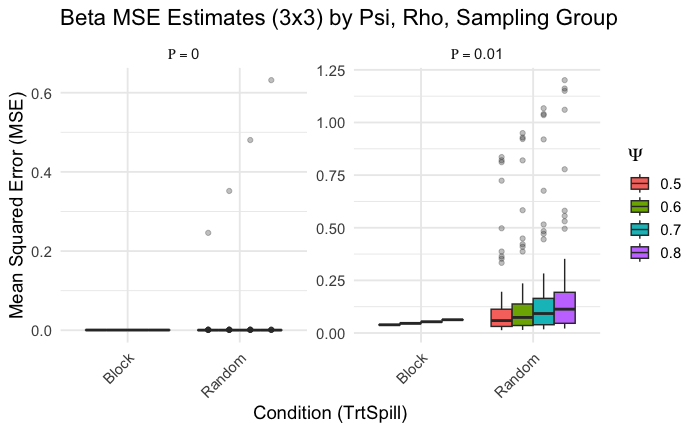
\includegraphics[width=\linewidth]{figures/BetaMSEresults/BetaMSEtrtSpill3x3.png}
%DIF <          % \caption{3x3 spatial grid of intervention (red) and control (blue) clusters assigned via Simple Random Sampling}
%DIF <          % \label{figure:BetaMSEtrtSpill3x3}
%DIF <      \end{minipage}
%DIFDELCMD < 

%DIFDELCMD < %%%
%DIF <      % Overall figure caption
%DIF <      \caption{Intervention effect MSE for 3x3 cluster grid with spillover allowed on control and intervention clusters}
%DIF <      \label{figure:BetaMSE3x3}
%DIF <  \end{figure}
%DIFDELCMD < 

%DIFDELCMD < %%%
%DIF <  --- Figure: Consolidated Intervention MSE for 3x3 grid ---
%DIFDELCMD < \begin{figure} [%%%
\DIFdelFL{!ht}%DIFDELCMD < ]
%DIFDELCMD < \centering
%DIFDELCMD < 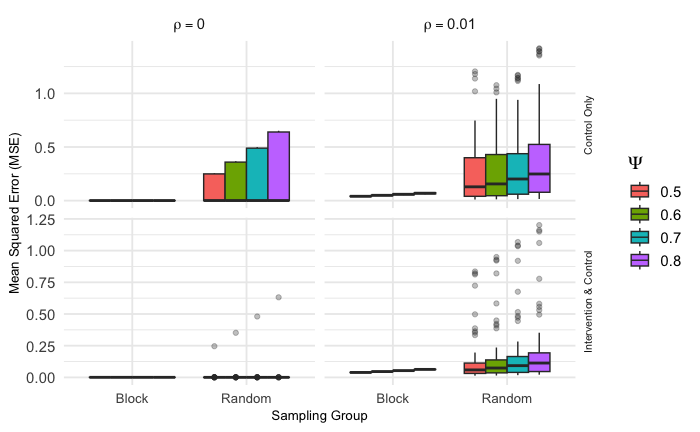
\includegraphics[width=0.80\textwidth]{figures/BetaMSEresults/MSE_Estimates_3x3.png}
%DIFDELCMD < %%%
%DIFDELCMD < \caption{%
{%DIFAUXCMD
\DIFdelFL{Intervention effect MSE for 3x3 cluster grid grouped by spillover effect magnitude, spatial dependence, sampling design, and spillover application type}}
%DIFAUXCMD
%DIFDELCMD < \label{figure:BetaMSE3x3Grouped}
%DIFDELCMD < \end{figure}
%DIFDELCMD < 

%DIFDELCMD < %%%
%DIF <  --- Table: Results for 3x3 Grid ---
%DIF <  \begin{table}[ht!]
%DIF <  \centering % Use \centering for better vertical spacing
%DIF <  \begin{tabular}{ l c c ccc ccc } % 'l' for left-aligned, 'c' for center-aligned
%DIF <      \toprule % Top rule from booktabs package
%DIF <      \textbf{\makecell{Spillover \\ Application}} & \textbf{\makecell{Spatial \\ Dependence \\ ($\rho$)}} & \textbf{\makecell{Spillover \\ Effect \\ ($\psi$)}} & \multicolumn{3}{c}{\textbf{\makecell{Simple Random\\ Sampling}}} & \multicolumn{3}{c}{\textbf{\makecell{Block Stratified\\ Sampling}}} \\
%DIF <      \cmidrule(lr){4-6} \cmidrule(lr){7-9} % Partial rules for sub-headers
%DIF <      & & & MSE & SD & Bias & MSE & SD & Bias \\
%DIF <      \midrule % Mid rule from booktabs package
%DIF <      \multirow{8}{*}{\makecell{Control Only\\ Spillover}} & \multirow{4}{*}{\makecell{Yes ($0.01$)}} & 0.5 & 0.23379 & 0.25927 & -0.05399 & 0.04054 & 0.00440 & -0.01229 \\
%DIF <      & & 0.6 & 0.27638 & 0.28599 & -0.09229 & 0.04960 & 0.00797 & -0.01773 \\
%DIF <      & & 0.7 & 0.32234 & 0.32838 & -0.13104 & 0.05919 & 0.01144 & -0.02204 \\
%DIF <      & & 0.8 & 0.37154 & 0.38566 & -0.16998 & 0.06920 & 0.01446 & -0.02516 \\
%DIF <      \cmidrule(lr){2-9} % Horizontal line spanning from Spatial Dependence to the end
%DIF <      & \multirow{4}{*}{\makecell{No ($0.00$)}} & 0.5 & 0.09200 & 0.12071 & -0.18211 & 0.00069 & 0.00020 & 0.00280 \\
%DIF <      & & 0.6 & 0.13221 & 0.17397 & -0.21877 & 0.00070 & 0.00018 & 0.00289 \\
%DIF <      & & 0.7 & 0.17980 & 0.23701 & -0.25545 & 0.00071 & 0.00017 & 0.00298 \\
%DIF <      & & 0.8 & 0.23485 & 0.30992 & -0.29217 & 0.00071 & 0.00017 & 0.00305 \\
%DIF <      \midrule % Mid rule to separate spillover applications
%DIF <      \multirow{8}{*}{\makecell{Intervention \&\\ Control Spillover}} & \multirow{4}{*}{\makecell{Yes ($0.01$)}} & 0.5 & 0.10339 & 0.14801 & 0.07140 & 0.03899 & 0.00222 & -0.01899 \\
%DIF <      & & 0.6 & 0.12214 & 0.16878 & 0.08204 & 0.04588 & 0.00271 & -0.02000 \\
%DIF <      & & 0.7 & 0.14332 & 0.19051 & 0.09237 & 0.05355 & 0.00319 & -0.02101 \\
%DIF <      & & 0.8 & 0.16807 & 0.21492 & 0.10133 & 0.06303 & 0.00074 & -0.01899 \\
%DIF <      \cmidrule(lr){2-9}
%DIF <      & \multirow{4}{*}{\makecell{No ($0.00$)}} & 0.5 & 0.00233 & 0.02188 & -0.00357 & 0.00052 & 0.00044 & 0.00383 \\
%DIF <      & & 0.6 & 0.00318 & 0.03131 & -0.00437 & 0.00052 & 0.00044 & 0.00383 \\
%DIF <      & & 0.7 & 0.00420 & 0.04276 & -0.00518 & 0.00052 & 0.00044 & 0.00383 \\
%DIF <      & & 0.8 & 0.00541 & 0.05624 & -0.00600 & 0.00052 & 0.00044 & 0.00383 \\
%DIF <      \bottomrule % Bottom rule from booktabs package
%DIF <  \end{tabular}
%DIF <  \caption{SRS vs. BSS: Intervention Effect Error Estimates - 3x3 Spatial Grid Setting}
%DIF <  \label{table:InterventionEstimates3x3}
%DIF <  \end{table}
%DIFDELCMD < 

%DIFDELCMD < \begin{table}[ht!]
%DIFDELCMD < \centering
%DIFDELCMD < \begin{tabular}{l c c ccc ccc}
%DIFDELCMD <     \toprule
%DIFDELCMD <     \textbf{\makecell{Spillover \\ Application}} & \textbf{\makecell{Spatial \\ Dependence \\ ($\rho$)}} & \textbf{\makecell{Spillover \\ Effect \\ ($\psi$)}} & \multicolumn{3}{c}{\textbf{\makecell{Simple Random\\ Sampling}}} & \multicolumn{3}{c}{\textbf{\makecell{Block Stratified\\ Sampling}}} \\
%DIFDELCMD <     \cmidrule(lr){4-6} \cmidrule(lr){7-9}
%DIFDELCMD <     & & & MSE & \makecell{SD \\ ($\times 10$)} & Bias & MSE & \makecell{SD \\ ($\times 10$)} & Bias \\
%DIFDELCMD <     \midrule
%DIFDELCMD <     \multirow{8}{*}{\makecell{Control Only\\ Spillover}} & \multirow{4}{*}{\makecell{Yes ($0.01$)}} & 0.5 & 0.234 & 2.593 & -0.054 & 0.041 & 0.044 & -0.012 \\
%DIFDELCMD <     & & 0.6 & 0.276 & 2.860 & -0.092 & 0.050 & 0.080 & -0.018 \\
%DIFDELCMD <     & & 0.7 & 0.322 & 3.284 & -0.131 & 0.059 & 0.114 & -0.022 \\
%DIFDELCMD <     & & 0.8 & 0.372 & 3.857 & -0.170 & 0.069 & 0.145 & -0.025 \\
%DIFDELCMD <     \cmidrule(lr){2-9}
%DIFDELCMD <     & \multirow{4}{*}{\makecell{No ($0$)}} & 0.5 & 0.092 & 1.207 & -0.182 & 0.001 & 0.002 & 0.003 \\
%DIFDELCMD <     & & 0.6 & 0.132 & 1.740 & -0.219 & 0.001 & 0.002 & 0.003 \\
%DIFDELCMD <     & & 0.7 & 0.180 & 2.370 & -0.255 & 0.001 & 0.002 & 0.003 \\
%DIFDELCMD <     & & 0.8 & 0.235 & 3.099 & -0.292 & 0.001 & 0.002 & 0.003 \\
%DIFDELCMD <     \midrule
%DIFDELCMD <     \multirow{8}{*}{\makecell{Intervention \&\\ Control Spillover}} & \multirow{4}{*}{\makecell{Yes ($0.01$)}} & 0.5 & 0.103 & 1.480 & 0.071 & 0.039 & 0.022 & -0.019 \\
%DIFDELCMD <     & & 0.6 & 0.122 & 1.688 & 0.082 & 0.046 & 0.027 & -0.020 \\
%DIFDELCMD <     & & 0.7 & 0.143 & 1.905 & 0.092 & 0.054 & 0.032 & -0.021 \\
%DIFDELCMD <     & & 0.8 & 0.168 & 2.149 & 0.101 & 0.063 & 0.007 & -0.019 \\
%DIFDELCMD <     \cmidrule(lr){2-9}
%DIFDELCMD <     & \multirow{4}{*}{\makecell{No ($0$)}} & 0.5 & 0.002 & 0.219 & -0.004 & 0.001 & 0.004 & 0.004 \\
%DIFDELCMD <     & & 0.6 & 0.003 & 0.313 & -0.004 & 0.001 & 0.004 & 0.004 \\
%DIFDELCMD <     & & 0.7 & 0.004 & 0.428 & -0.005 & 0.001 & 0.004 & 0.004 \\
%DIFDELCMD <     & & 0.8 & 0.005 & 0.562 & -0.006 & 0.001 & 0.004 & 0.004 \\
%DIFDELCMD <     \bottomrule
%DIFDELCMD < \end{tabular}
%DIFDELCMD < %%%
%DIFDELCMD < \caption{%
{%DIFAUXCMD
\DIFdelFL{SRS vs. BSS: Intervention Effect Error Estimates - 3x3 Spatial Grid Setting}}
%DIFAUXCMD
%DIFDELCMD < \label{table:InterventionEstimates3x3}
%DIFDELCMD < \end{table}
%DIFDELCMD < 

%DIFDELCMD < %%%
%DIF <  \pagebreak
%DIFDELCMD < 

%DIFDELCMD < %%%
\subsection{\DIFdel{Intervention Effect Estimates (3x4 grid)}}
%DIFAUXCMD
\addtocounter{subsection}{-1}%DIFAUXCMD
%DIFDELCMD < 

%DIFDELCMD < %%%
%DIF <  R1.5: Risk-management framing (3x4 grid); R2.M4 checkerboard paradox noted
\DIFdel{Table~3 and Figure~\ref{figure:BetaMSE3x4Grouped} present the intervention effect estimates for the 3$\times$4 spatial grid. These results reveal both the typical strengths of BSS and a notable exception that illuminates the limits of the checkerboard design.
}%DIFDELCMD < 

%DIFDELCMD < %%%
\DIFdel{Under the Control Clusters Only (TrtNoSpill) spillover condition, BSS dramatically outperforms SRS across all combinations of $\rho$ }\DIFdelend \DIFaddbegin \DIFadd{Table~\ref{table:AllocationCounts} summarizes the resulting allocation spaces, }\DIFaddend and \DIFdelbegin \DIFdel{$\psi$. With no spatial dependence ($\rho = 0$) , BSS MSE is an order of magnitude smaller than SRS (e.g., BSS MSE $\approx 0.0004$ vs. SRS MSE $= 0.034$ at $\psi = 0.5$). With spatial dependence ($\rho = 0.01$), BSS retains a substantial advantage (e.g., BSS MSE $\approx 0.035$ vs. SRS MSE $= 0.120$ at $\psi = 0.5$). BSS SD is near zero throughout, while SRS SD is substantially larger---confirming that the two valid BSS checkerboard allocations for this grid provide stable and consistently low-error estimates whenever spillover is confined to control clusters.
}%DIFDELCMD < 

%DIFDELCMD < %%%
\DIFdel{Under the Intervention \& Control Clusters (TrtSpill) spillover condition, results are more nuanced. With no spatial dependence ($\rho = 0$), BSS achieves lower MSE than SRS (e.g., BSS MSE $\approx 0.0003$ vs. SRS MSE $= 0.001$ at $\psi = 0.5$) . However, when spatial dependence is present ($\rho = 0.01$), BSS MSE ($\approx 0.223$ at $\psi = 0.5$) substantially exceeds SRS MSE ($= 0.112$). This inversion occurs because the strict checkerboard structure of the 3$\times$4 BSS allocation ensures that every intervention cluster is surrounded entirely by control neighbors eligible for spillover; under TrtSpill, this configuration amplifies the systematic bias in $\hat{\beta}$, a ``checkerboard paradox" discussed further in Section~\ref{section:Discussion}.
}%DIFDELCMD < 

%DIFDELCMD < %%%
\DIFdel{Across all gridsizes, increasing $\psi$ consistently raises MSE for both methods, and the presence of spatial dependence ($\rho = 0.01$) further inflates MSE relative to the $\rho = 0$ setting. The 3$\times$4 results reinforce the broader conclusion: BSS reliably bounds worst-case estimation error under TrtNoSpill, while the TrtSpill regime with spatial dependence represents the primary scenario in which a practitioner should carefully weigh the risk-management benefits of BSS against its potential for amplified bias}\DIFdelend \DIFaddbegin \DIFadd{Figure~\ref{figure:GridsCombined} shows a representative BSS (top row) and SRS (bottom row) allocation for each grid}\DIFaddend . \DIFaddbegin \DIFadd{The spatial objects are constructed with the Simple Features for R package\mbox{%DIFAUXCMD
\cite{pebesma_simple_2018}}\hskip0pt%DIFAUXCMD
\mbox{%DIFAUXCMD
\cite{pebesma_spatial_2023}}\hskip0pt%DIFAUXCMD
.
}\DIFaddend 

%DIF <  --- Figure: Beta MSE for 3x4 (side by side) ---
%DIF <  \begin{figure}[!ht]
%DIF <      \centering % Centers the entire block of minipages
\DIFdelbegin %DIFDELCMD < 

%DIFDELCMD < %%%
%DIF <      % Left Column Figure
%DIF <      \begin{minipage}{0.45\textwidth} % Minipage for the left figure
%DIF <          \centering % Centers image within its minipage
%DIF <          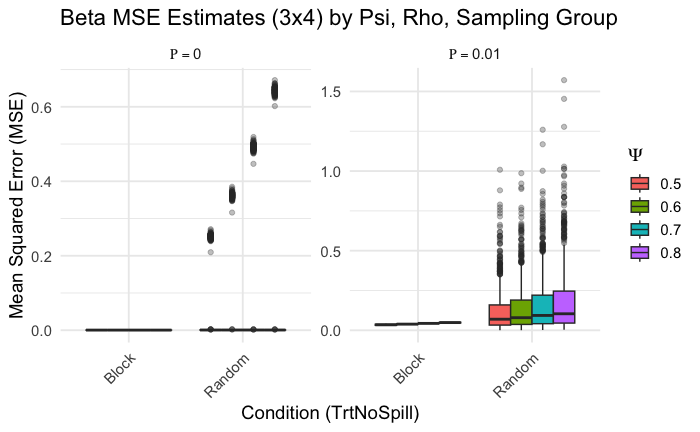
\includegraphics[width=\linewidth]{figures/BetaMSEresults/BetaMSEtrtNoSpill3x4.png}
%DIF <          % \caption{Intervention effect MSE for 3x4 cluster grid with spillover allowed only on control clusters}
%DIF <          % \label{figure:BetaMSEtrtNoSpill3x4}
%DIF <      \end{minipage}%\hspace*{\fill}%  <--- CRITICAL: Ensure NO actual newline character, blank line, or extra spaces between this '%' and the '\begin{minipage}' below. This entire sequence should be one continuous "line" in your .tex file.
%DIF <      \hfill % \hfill puts a flexible horizontal space between minipages
%DIF <      \begin{minipage}{0.45\textwidth} % Minipage for the right figure
%DIF <          \centering % Centers image within its minipage
%DIF <          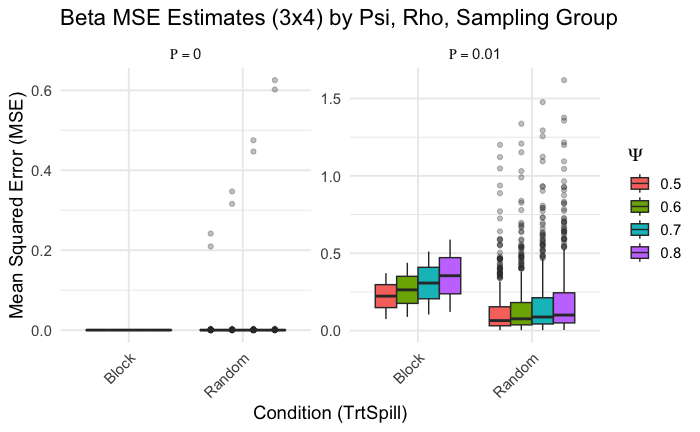
\includegraphics[width=\linewidth]{figures/BetaMSEresults/BetaMSEtrtSpill3x4.png}
%DIF <          % \caption{3x4 spatial grid of intervention (red) and control (blue) clusters assigned via Simple Random Sampling}
%DIF <          % \label{figure:BetaMSEtrtSpill3x4}
%DIF <      \end{minipage}
%DIFDELCMD < 

%DIFDELCMD < %%%
%DIF <      % Overall figure caption
%DIF <      \caption{Intervention effect MSE for 3x4 cluster grid with spillover allowed on control and intervention clusters}
%DIF <      \label{figure:BetaMSE3x4}
%DIF <  \end{figure}
%DIFDELCMD < 

%DIFDELCMD < %%%
%DIF <  --- Figure: Consolidated Intervention MSE for 3x4 grid ---
%DIFDELCMD < \begin{figure} [%%%
\DIFdelFL{!ht}%DIFDELCMD < ]
%DIFDELCMD < \centering
%DIFDELCMD < 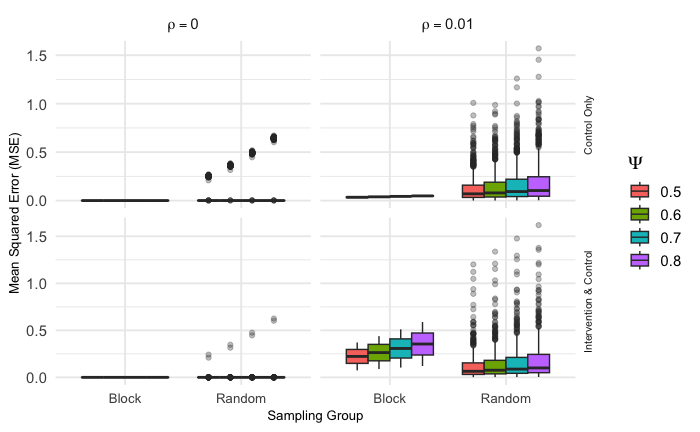
\includegraphics[width=0.80\textwidth]{figures/BetaMSEresults/MSE_Estimates_3x4.png}
%DIFDELCMD < %%%
%DIFDELCMD < \caption{%
{%DIFAUXCMD
\DIFdelFL{Intervention effect MSE for 3x4 cluster grid grouped by spillover effect magnitude, spatial dependence, sampling design, and spillover application type}}
%DIFAUXCMD
%DIFDELCMD < \label{figure:BetaMSE3x4Grouped}
%DIFDELCMD < \end{figure}
%DIFDELCMD < 

%DIFDELCMD < %%%
%DIF <  --- Table: Results for 3x4 Grid ---
%DIF <  \begin{table}[ht!]
%DIF <  \centering % Use \centering for better vertical spacing
%DIF <  \begin{tabular}{ l c c ccc ccc } % 'l' for left-aligned, 'c' for center-aligned
%DIF <      \toprule % Top rule from booktabs package
%DIF <      \textbf{\makecell{Spillover \\ Application}} & \textbf{\makecell{Spatial \\ Dependence \\ ($\rho$)}} & \textbf{\makecell{Spillover \\ Effect \\ ($\psi$)}} & \multicolumn{3}{c}{\textbf{\makecell{Simple Random\\ Sampling}}} & \multicolumn{3}{c}{\textbf{\makecell{Block Stratified\\ Sampling}}} \\
%DIF <      \cmidrule(lr){4-6} \cmidrule(lr){7-9} % Partial rules for sub-headers
%DIF <      & & & MSE & SD & Bias & MSE & SD & Bias \\
%DIF <      \midrule % Mid rule from booktabs package
%DIF <      \multirow{8}{*}{\makecell{Control Only\\ Spillover}} & \multirow{4}{*}{\makecell{Yes ($0.01$)}} & 0.5 & 0.12009 & 0.13244 & 0.03254 & 0.03463 & 0.00963 & -0.15200 \\
%DIF <      & & 0.6 & 0.13800 & 0.14807 & 0.02057 & 0.03881 & 0.00505 & -0.16651 \\
%DIF <      & & 0.7 & 0.15902 & 0.17166 & 0.00943 & 0.04345 & 0.00011 & -0.18039 \\
%DIF <      & & 0.8 & 0.18330 & 0.20387 & -0.00075 & 0.04842 & 0.00561 & -0.19332 \\
%DIF <      \cmidrule(lr){2-9} % Horizontal line spanning from Spatial Dependence to the end
%DIF <      & \multirow{4}{*}{\makecell{No ($0.00$)}} & 0.5 & 0.03425 & 0.08554 & -0.06751 & 0.00036 & 0.00022 & -0.00571 \\
%DIF <      & & 0.6 & 0.04905 & 0.12318 & -0.08097 & 0.00036 & 0.00022 & -0.00563 \\
%DIF <      & & 0.7 & 0.06666 & 0.16769 & -0.09444 & 0.00035 & 0.00020 & -0.00555 \\
%DIF <      & & 0.8 & 0.08678 & 0.21912 & -0.10791 & 0.00034 & 0.00016 & -0.00553 \\
%DIF <      \midrule % Mid rule to separate spillover applications
%DIF <      \multirow{8}{*}{\makecell{Intervention \&\\ Control Spillover}} & \multirow{4}{*}{\makecell{Yes ($0.01$)}} & 0.5 & 0.11193 & 0.12873 & 0.02201 & 0.22286 & 0.20995 & -0.41486 \\
%DIF <      & & 0.6 & 0.13069 & 0.14762 & 0.02096 & 0.26343 & 0.24750 & -0.45154 \\
%DIF <      & & 0.7 & 0.15112 & 0.16817 & 0.01963 & 0.30741 & 0.28774 & -0.48833 \\
%DIF <      & & 0.8 & 0.17323 & 0.19046 & 0.01810 & 0.35475 & 0.33060 & -0.52516 \\
%DIF <      \cmidrule(lr){2-9}
%DIF <      & \multirow{4}{*}{\makecell{No ($0.00$)}} & 0.5 & 0.00073 & 0.01051 & -0.00126 & 0.00028 & 0.00004 & -0.00251 \\
%DIF <      & & 0.6 & 0.00096 & 0.01542 & -0.00149 & 0.00029 & 0.00004 & -0.00241 \\
%DIF <      & & 0.7 & 0.00124 & 0.02143 & -0.00172 & 0.00030 & 0.00005 & -0.00232 \\
%DIF <      & & 0.8 & 0.00158 & 0.02853 & -0.00194 & 0.00031 & 0.00005 & -0.00224 \\
%DIF <      \bottomrule % Bottom rule from booktabs package
%DIF <  \end{tabular}
%DIF <  \caption{SRS vs. BSS: Intervention Effect Error Estimates - 3x4 Spatial Grid Setting}
%DIF <  \label{table:InterventionEstimates3x4}
%DIF <  \end{table}
%DIFDELCMD < 

%DIFDELCMD < \begin{table}[ht!]
%DIFDELCMD < \centering
%DIFDELCMD < \begin{tabular}{l c c ccc ccc}
%DIFDELCMD <     \toprule
%DIFDELCMD <     \textbf{\makecell{Spillover \\ Application}} & \textbf{\makecell{Spatial \\ Dependence \\ ($\rho$)}} & \textbf{\makecell{Spillover \\ Effect \\ ($\psi$)}} & \multicolumn{3}{c}{\textbf{\makecell{Simple Random\\ Sampling}}} & \multicolumn{3}{c}{\textbf{\makecell{Block Stratified\\ Sampling}}} \\
%DIFDELCMD <     \cmidrule(lr){4-6} \cmidrule(lr){7-9}
%DIFDELCMD <     & & & MSE & \makecell{SD \\($\times 100$)} & Bias & \makecell{MSE \\($\times 10$)} & \makecell{SD \\($\times 100$)} & Bias \\
%DIFDELCMD <     \midrule
%DIFDELCMD <     \multirow{8}{*}{\makecell{Control Only\\ Spillover}} & \multirow{4}{*}{\makecell{Yes ($0.01$)}} & 0.5 & 0.120 & 13.244 & 0.033 & 0.346 & 0.963 & -0.152 \\
%DIFDELCMD <     & & 0.6 & 0.138 & 14.807 & 0.021 & 0.388 & 0.505 & -0.167 \\
%DIFDELCMD <     & & 0.7 & 0.159 & 17.166 & 0.009 & 0.435 & 0.011 & -0.180 \\
%DIFDELCMD <     & & 0.8 & 0.183 & 20.387 & -0.001 & 0.484 & 0.561 & -0.193 \\
%DIFDELCMD <     \cmidrule(lr){2-9}
%DIFDELCMD <     & \multirow{4}{*}{\makecell{No ($0$)}} & 0.5 & 0.034 & 8.554 & -0.068 & 0.004 & 0.022 & -0.006 \\
%DIFDELCMD <     & & 0.6 & 0.049 & 12.318 & -0.081 & 0.004 & 0.022 & -0.006 \\
%DIFDELCMD <     & & 0.7 & 0.067 & 16.769 & -0.094 & 0.004 & 0.020 & -0.006 \\
%DIFDELCMD <     & & 0.8 & 0.087 & 21.912 & -0.108 & 0.003 & 0.016 & -0.006 \\
%DIFDELCMD <     \midrule
%DIFDELCMD <     \multirow{8}{*}{\makecell{Intervention \&\\ Control Spillover}} & \multirow{4}{*}{\makecell{Yes ($0.01$)}} & 0.5 & 0.112 & 12.873 & 0.022 & 2.229 & 20.995 & -0.415 \\
%DIFDELCMD <     & & 0.6 & 0.131 & 14.762 & 0.021 & 2.634 & 24.750 & -0.452 \\
%DIFDELCMD <     & & 0.7 & 0.151 & 16.817 & 0.020 & 3.074 & 28.774 & -0.488 \\
%DIFDELCMD <     & & 0.8 & 0.173 & 19.046 & 0.018 & 3.548 & 33.060 & -0.525 \\
%DIFDELCMD <     \cmidrule(lr){2-9}
%DIFDELCMD <     & \multirow{4}{*}{\makecell{No ($0$)}} & 0.5 & 0.001 & 1.051 & -0.001 & 0.003 & 0.004 & -0.003 \\
%DIFDELCMD <     & & 0.6 & 0.001 & 1.542 & -0.001 & 0.003 & 0.004 & -0.002 \\
%DIFDELCMD <     & & 0.7 & 0.001 & 2.143 & -0.002 & 0.003 & 0.005 & -0.002 \\
%DIFDELCMD <     & & 0.8 & 0.002 & 2.853 & -0.002 & 0.003 & 0.005 & -0.002 \\
%DIFDELCMD <     \bottomrule
%DIFDELCMD < \end{tabular}
%DIFDELCMD < %%%
%DIFDELCMD < \caption{%
{%DIFAUXCMD
\DIFdelFL{SRS vs. BSS: Intervention Effect Error Estimates - 3x4 Spatial Grid Setting}}
%DIFAUXCMD
%DIFDELCMD < \label{table:InterventionEstimates3x4}
%DIFDELCMD < \end{table}
%DIFDELCMD < 

%DIFDELCMD < %%%
%DIF <  \pagebreak
%DIFDELCMD < 

%DIFDELCMD < %%%
%DIF <  \subsection{Intervention Effect Estimates (Control Only Spillover)}
%DIFDELCMD < 

%DIFDELCMD < %%%
%DIF <  \begin{figure} [!ht]
%DIF <  \centering
%DIF <  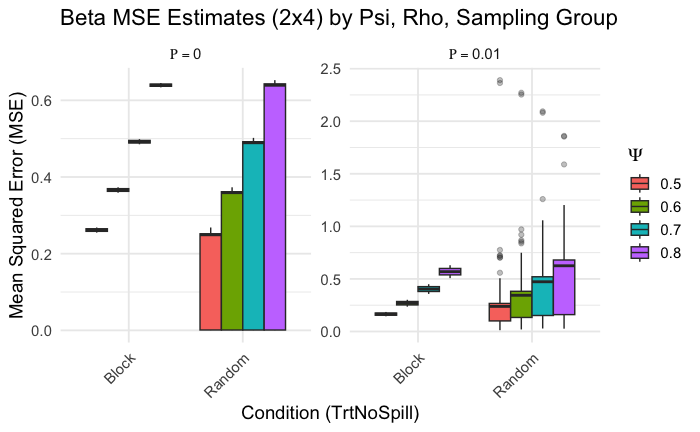
\includegraphics[width=0.60\textwidth]{figures/BetaMSEresults/BetaMSEtrtNoSpill2x4.png}
%DIF <  \caption{Intervention effect MSE for 2x4 cluster grid with spillover allowed only on control clusters}
%DIF <  \label{figure:BetaMSEtrtNoSpill2x4}
%DIF <  \end{figure}
%DIFDELCMD < 

%DIFDELCMD < %%%
%DIF <  \begin{figure} [!ht]
%DIF <  \centering
%DIF <  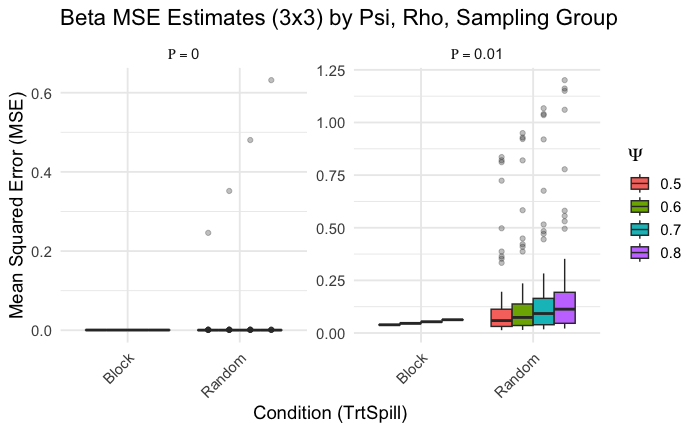
\includegraphics[width=0.60\textwidth]{figures/BetaMSEresults/BetaMSEtrtSpill3x3.png}
%DIF <  \caption{Intervention effect MSE for 3x3 cluster grid with spillover allowed only on control clusters}
%DIF <  \label{figure:BetaMSEtrtSpill3x3}
%DIF <  \end{figure}
%DIFDELCMD < 

%DIFDELCMD < %%%
%DIF <  \begin{figure} [!ht]
%DIF <  \centering
%DIF <  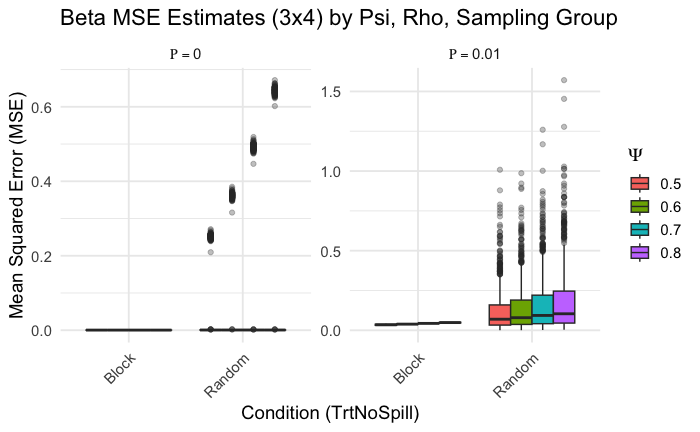
\includegraphics[width=0.60\textwidth]{figures/BetaMSEresults/BetaMSEtrtNoSpill3x4.png}
%DIF <  \caption{Intervention effect MSE for 3x4 cluster grid with spillover allowed only on control clusters}
%DIF <  \label{figure:BetaMSEtrtNoSpill3x4}
%DIF <  \end{figure}
%DIFDELCMD < 

%DIFDELCMD < %%%
%DIF <  \subsection{Intervention Effect Estimates (Intervention \& Control Spillover)}
%DIFDELCMD < 

%DIFDELCMD < %%%
%DIF <  \begin{figure} [!ht]
%DIF <  \centering
%DIF <  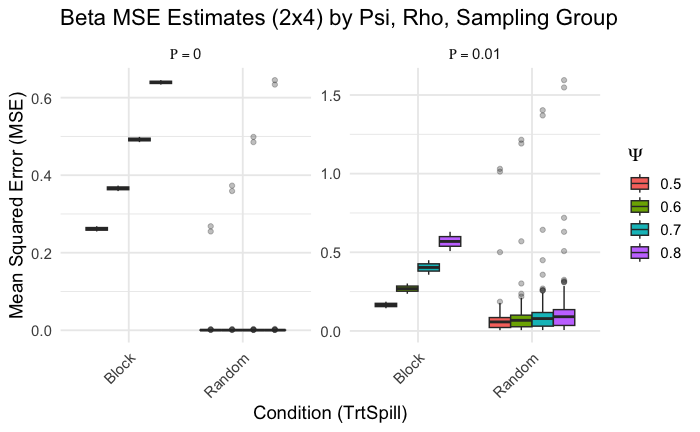
\includegraphics[width=0.60\textwidth]{figures/BetaMSEresults/BetaMSEtrtSpill2x4.png}
%DIF <  \caption{Intervention effect MSE for 2x4 cluster grid with spillover allowed on control and intervention clusters}
%DIF <  \label{figure:BetaMSEtrtSpill2x4}
%DIF <  \end{figure}
%DIFDELCMD < 

%DIFDELCMD < %%%
%DIF <  \begin{figure} [!ht]
%DIF <  \centering
%DIF <  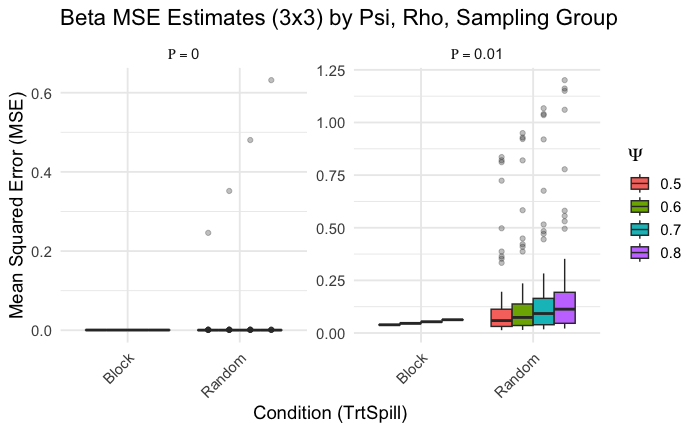
\includegraphics[width=0.60\textwidth]{figures/BetaMSEresults/BetaMSEtrtSpill3x3.png}
%DIF <  \caption{Intervention effect MSE for 3x3 cluster grid with spillover allowed on control and intervention clusters}
%DIF <  \label{figure:BetaMSEtrtSpill3x3}
%DIF <  \end{figure}
%DIFDELCMD < 

%DIFDELCMD < %%%
%DIF <  \begin{figure} [!ht]
%DIF <  \centering
%DIF <  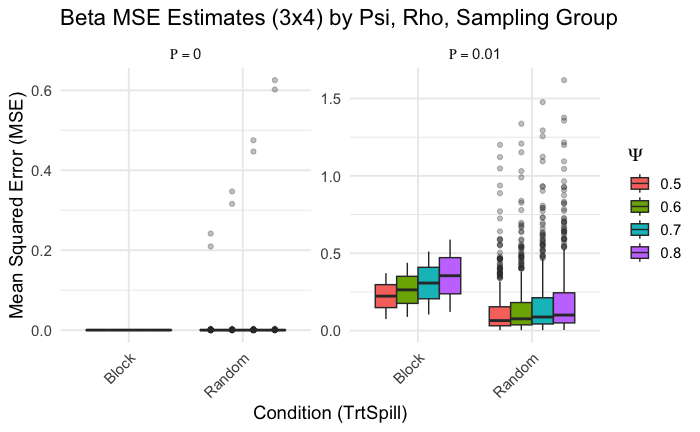
\includegraphics[width=0.60\textwidth]{figures/BetaMSEresults/BetaMSEtrtSpill3x4.png}
%DIF <  \caption{Intervention effect MSE for 3x4 cluster grid with spillover allowed on control and intervention clusters}
%DIF <  \label{figure:BetaMSEtrtSpill3x4}
%DIF <  \end{figure}
%DIFDELCMD < 

%DIFDELCMD < %%%
%DIF <  \subsection{Comparison of Methods}
%DIFDELCMD < 

%DIFDELCMD < %%%
%DIF <  --- GA Study APPLICATION (application in practice) ---
\DIFdelend \section{Application}

The findings from our simulation study provide relevant insights for investigators designing CRTs in real-world applications where spatial dependence and spillover effects are present and must be accounted for. In this case, a pair of studies in development that we consider involve the North Carolina Department of Adult Correction. The structure of correctional systems, particularly community supervision, often involves geographically clustered units where staff from different clusters may interact and regional similarities can influence outcomes. The investigators leading these studies desire recommendations for treatment assignment methodology regarding the spatially clustered nature of their design.

\subsection{Background of Probation in North Carolina}

The North Carolina Department of Adult Correction Division of Community Supervision (NC DCS) provides a clear example of a spatially structured organization, making it an ideal context for applying our research. The NC DCS is organized into four geographic Divisions numbered 1 through 4 from East to West, which are subdivided into 30 Districts that make up the entirety of the state. Each district is composed of one or more counties. If there is more than one county in the district, the counties are adjacent, but some districts are composed of only a singular county. In these districts, Probation and Parole Officers (PPOs) supervise individuals at the county level and are themselves managed by Chief Probation/Parole Officers (CPPOs) and Judicial District Managers (JDMs) who oversee districts. Each division (composed of multiple districts) is managed by a Judicial Division Director (JD Dir) as well. A map of the segmentation of each division and district is presented in Figure~\ref{figure:NCDCS_map}.

\begin{figure} [!ht]
\centering
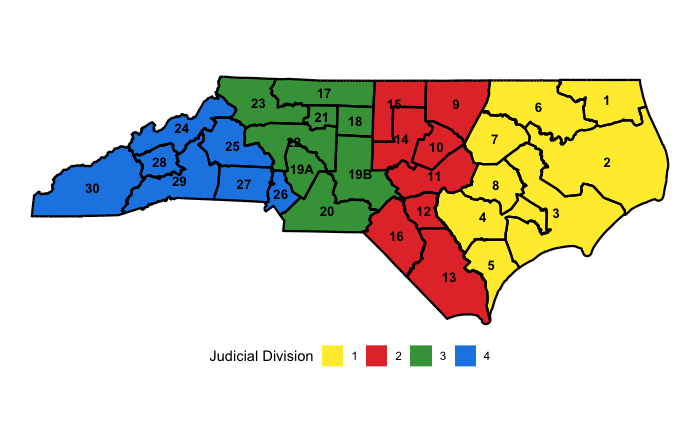
\includegraphics[width=0.80\textwidth]{figures/Applications/NC_DCS_Map_NoCounties.png}
\caption{The North Carolina Department of Adult Correction Division of Community Supervision map is segmented into 30 judicial districts that are grouped into 4 judicial divisions.}
\label{figure:NCDCS_map}
\end{figure}

This geographic and administrative structure means that Chiefs and Judicial District Managers (JDMs) often span multiple units and counties, creating a direct channel for spillover effects among regions under their supervision. For instance, if leadership views an intervention in one county favorably, they may implement its components in other counties under their jurisdiction, even if those areas were not assigned the intervention. Furthermore, adjacent counties within the same region often share demographic characteristics, labor market conditions, and similar judicial cultures, as well as the same managed care organizations and treatment providers, leading to spatial dependence in probation outcomes. The choice of treatment assignment sampling strategy in this context is non-trivial when considering potential options of either simple random sampling (SRS) or block-stratified sampling (BSS). Selection of the appropriate treatment sampling strategy may yield beneficial downstream outcomes when considering the error of intervention \& spillover estimates.

\subsection{Case 1: Trauma-Informed and Engaged Supervision}

One proposed study involves implementing a trauma-informed supervision model for PPOs managing specialty caseloads like domestic violence, sex offender, or gang affiliated cases. The intervention consists of intensive training and follow-up sessions delivered to cohorts of PPOs and CPPOs. The primary outcomes would be changes in officer knowledge and attitudes, as well as impacts on individuals under their supervision. The key design decision for this study is the unit of randomization. Randomizing at the PPO level is not feasible due to the high likelihood of spillover within a county office. Therefore, a cluster randomized design at the county or district level is necessary. This cluster randomization decision is also supported by agency-related logistics in addition to considerations for spillover. Original plans for a similar study, acknowledging the risk of contamination between adjacent units, considered randomization at the district level specifically to minimize spillover. This scenario directly reflects the conditions modeled in our simulation, where the effectiveness of an intervention in one cluster may influence outcomes in neighboring control clusters where an intervention is not applied.

\subsection{Case 2: Testing an implementation strategy for specialty mental health probation}

Another study proposal aims to test a strategy for improving the implementation of Specialty Mental Health Probation (SMHP). The intervention involves enhancing collaboration between PPOs and community-based behavioral health service providers through cross-training sessions and joint treatment team meetings. The primary outcome is improved collaboration, with secondary outcomes related to treatment engagement for individuals on probation. This case presents a more complex spatial challenge. In addition to the geographic proximity of probation districts, the behavioral health system in North Carolina is managed by four large Managed Care Organizations (MCOs), each responsible for a different coverage area. Some service provider agencies are large, operating in multiple counties and potentially across different MCO regions. This creates multiple, overlapping layers of potential spillover. Figure~\ref{figure:NCMCO_map} presents a map of which counties in the state that each MCO operates. An intervention implemented in one county could be adopted by a provider and informally carried into a neighboring control county, or an MCO could promote a similar initiative, confounding the study's results. This complex spatial linkage underscores the importance of a robust treatment assignment strategy in order to efficiently estimate the impact of the intervention.

\begin{figure} [!ht]
\centering
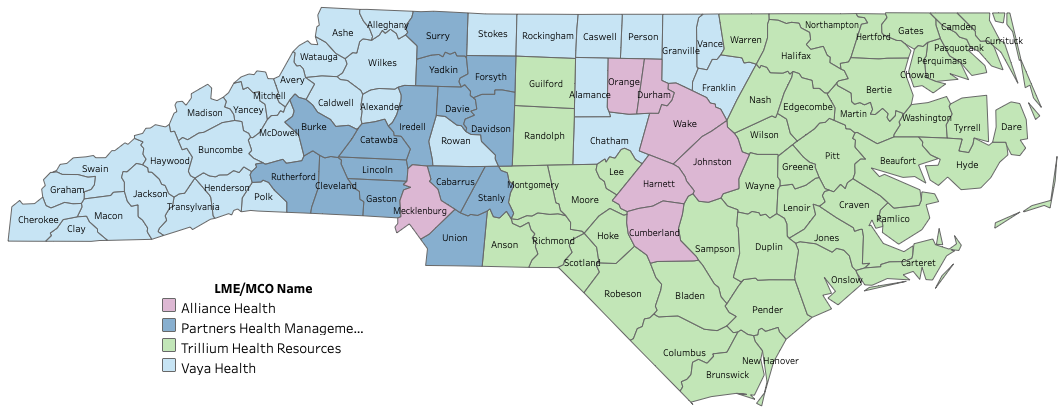
\includegraphics[width=0.80\textwidth]{figures/Applications/NC_MCO_Map.png}
\caption{Map of Local Management Entity/Managed Care Organizations (LME/MCOs) for each county in the state of North Carolina. There are 4 LME/MCOs of which one operates in each of the 100 counties of the state.}
\label{figure:NCMCO_map}
\end{figure}

\subsection{Recommendations for treatment assignment}
%DIF <  Simulation comparison of SRS vs. BSS & interpretation
The results of our simulation study indicate a clear trade-off: \DIFdelbegin \DIFdel{we previously concluded that }\DIFdelend Simple Random Sampling (SRS) reduces the average mean squared error (MSE) across many randomizations (intervention/control combinations), while Block Stratified Sampling (BSS) reduces the variance of the error although it is not minimized. Put simply, BSS is less likely to produce a ``perfect" assignment by chance but is also robust against a ``worst-case" assignment that could render the study results invalid. \DIFdelbegin \DIFdel{For }\DIFdelend \DIFaddbegin \DIFadd{We recommend BSS for }\DIFaddend both case studies presented, \DIFdelbegin \DIFdel{Block Stratified Sampling (BSS) is the recommended approach}\DIFdelend \DIFaddbegin \DIFadd{but with an important and explicit qualification: this recommendation rests on the expectation that spillover in these correctional-supervision settings flows primarily from intervention units into neighboring control units (the TrtNoSpill regime), where BSS reliably controls estimation variance. If investigators instead anticipate substantial bidirectional spillover among treated units together with background spatial dependence, our simulations show that the spatial separation enforced by BSS can amplify rather than reduce bias (the checkerboard paradox, Section~\ref{section:Discussion}); in that regime SRS, or an analysis-stage buffer-zone design, may be preferable. The recommendation below is therefore conditional on the anticipated spillover mechanism, and we encourage investigators to state that assumption explicitly when justifying their design}\DIFaddend .

%DIF <  Recommendation & rationale for study 1
In Case 1 (Trauma-Informed Supervision), a simple random assignment of districts could, by chance, result in a geographic imbalance, concentrating treated districts in one part of the state. This would confound the intervention effect with regional characteristics. A more robust design would be to stratify by the four state divisions and randomize districts to intervention and control conditions within each division with a block stratification strategy. This ensures geographic balance and leverages the finding that BSS minimizes estimation variance, providing a more stable and defensible estimate of the intervention effect.

%DIF < ERecommendation & rationale for study 2 (EDIT THIS SECTION!)
In Case 2 (SMHP Implementation), the rationale for BSS is even stronger due to the complex potential for spillover. A simple random assignment of counties would ignore the significant structural influence of the MCOs. The most effective design would be to stratify by MCO coverage area, randomizing counties to the implementation strategy (intervention) or control condition within each MCO. This approach directly controls for the significant confounding variable of MCO-level policies and provider networks. However, some challenges with this MCO stratification do persist. For example, it's possible that a county is selected for the intervention and is supervised by a CPPO or even a judicial district manager that oversees a control group county. Furthermore, multiple service providers may serve a given county in the coverage area of an MCO and it is possible that multiple service providers begin team meetings. Another consideration is that some service providers are very large and have offices around the state and contract with more than one MCO. Based on this, we must consider potential spillover if after participating in a treatment team meeting, a service provider intends initiate those practices in another part of the state. Given the high risk of contamination, the robustness of BSS in minimizing error variance makes it \DIFdelbegin \DIFdel{the most }\DIFdelend \DIFaddbegin \DIFadd{a }\DIFaddend prudent choice for achieving a reliable effect estimate\DIFaddbegin \DIFadd{, provided spillover is expected to flow chiefly into control units}\DIFaddend . While SRS might achieve a lower MSE (intervention error estimate) in theory, the risk of a single, poorly distributed randomization in a complex, real-world setting outweighs the potential benefit. \DIFdelbegin \DIFdel{Therefore, }\DIFdelend \DIFaddbegin \DIFadd{We note one caveat specific to this case: because the SMHP setting carries a genuine possibility of bidirectional spillover among treated units (e.g., a large provider carrying practices across MCO regions), investigators should weigh whether an analysis-stage buffer-zone exclusion of the most contamination-prone boundary counties would further protect the estimate---an option that, as discussed in Section~\ref{section:Discussion}, directly addresses the identifiability limitation rather than only its variance. Subject to that consideration, }\DIFaddend it is wise to proceed with a sampling strategy that \DIFdelbegin \DIFdel{aims to manage }\DIFdelend \DIFaddbegin \DIFadd{manages }\DIFaddend estimation error with minimal variation.

%DIF <  Describes sample BSS figure
A representation of this block stratified sampling strategy where we ``block" treatment and control districts together with an effort to isolate districts of a particular intervention status from each other is shown in Figure~\ref{figure:recommendation_map}. Note that across the entire map of the state and specifically in Judicial Division 1 (easternmost region) that when possible districts of the same intervention status are isolated from each other. When districts share a border with multiple other districts, this sampling method ensures that treatment districts are isolated from other treatment districts as best as possible. It is important to note that, unlike the idealized rectangular grids examined in the simulation study, real-world jurisdictions have irregular shapes and varying numbers of shared borders. The allocation depicted in Figure~\ref{figure:recommendation_map} therefore represents a \textit{best-effort} block stratification: the assignment minimizes shared borders between same-treatment districts while acknowledging that perfect spatial separation cannot always be achieved in practice. Investigators applying BSS to real-world geographic settings should expect some deviation from the strict no-common-edge criterion and should document the degree to which the chosen allocation approximates the ideal.

\begin{figure} [!ht]
\centering
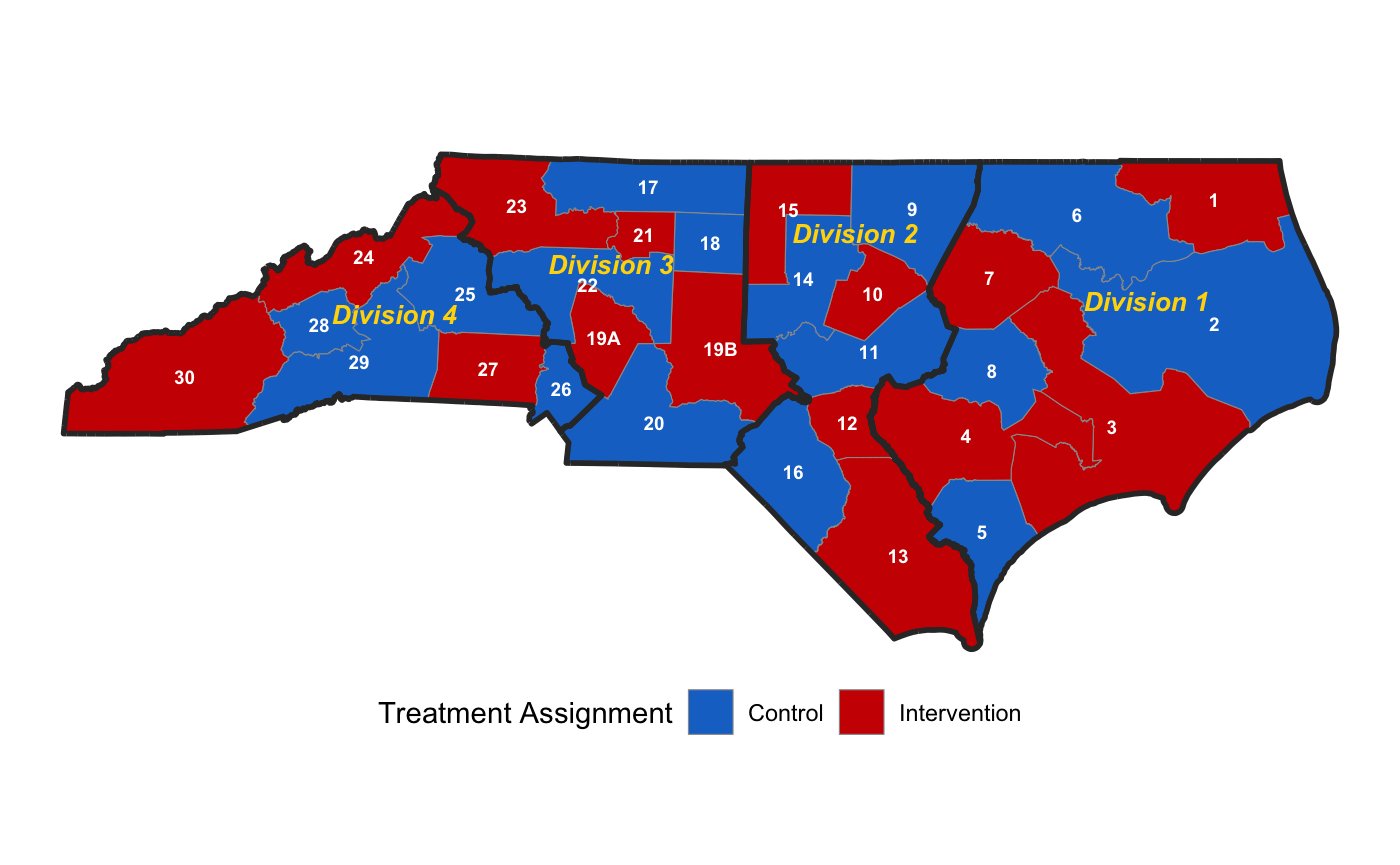
\includegraphics[width=0.80\textwidth]{figures/Applications/BSS_Assignments_NC_Map_Applications_Text_Labels.png}
\caption{Map of North Carolina with example block stratified sampling intervention assignments for each judicial district under consideration. Districts are assigned to either treatment (red) or control (blue).}
\label{figure:recommendation_map}
\end{figure}

%DIF <  --- DISCUSSION ---
\section{Discussion}\label{section:Discussion}

\subsection{Relevance of results}

This simulation study provides insights into the efficiency of treatment assignment methodologies in spatial cluster randomized trials (CRTs) when considering spillover effects and spatial dependence. A primary contribution of this work is the direct comparison between Simple Random Sampling (SRS) and Block Stratified Sampling (BSS) across various scenarios, offering practical guidance for investigators designing such trials.

%DIF <  R1.1 / R2.2 / R2.3 / R1.4: BSS novelty and McCann et al. (moved from Methods §2.4.3)
The spatial separation principle underlying BSS has antecedents in spatially balanced experimental designs. For example, McCann et al.~(2018) demonstrated that spatially stratified allocation in field trials reduces confounding by ensuring treatment balance across the spatial domain\cite{mccann_spatial_2018}. However, the formal comparison of SRS and BSS within the context of spatial cluster randomized trials that incorporate both a spatial autoregressive (SAR) model for background dependence \emph{and} an explicit spillover mechanism represents a novel contribution of the present work. To our knowledge, no prior study has examined how the choice between these two allocation strategies affects the bias--variance decomposition of the intervention effect estimator under SAR modeling with simultaneous spillover effects, nor has the exhaustive enumeration of all feasible allocations been used to characterize the full design space of a spatial CRT.

%DIF <  R2.6: Covariate-constrained randomization literature (moved from Methods §2.4.3)
A related line of work concerns covariate-constrained randomization, in which the set of eligible allocations is restricted to those achieving covariate balance across treatment arms\cite{crisp_covariate-constrained_2023}. While BSS and covariate-constrained randomization both restrict the allocation space, they operate on fundamentally different principles: BSS imposes a spatial isolation condition based on cluster adjacency (no two same-treatment clusters share a Rook boundary), whereas covariate-constrained randomization restricts allocations based on balance of measured covariates. These approaches are complementary and could in principle be combined; however, the present work focuses on the spatial isolation constraint as the design criterion, leaving covariate-balance extensions to future research.

\DIFdelbegin \DIFdel{Our findings show a clear relationship between the magnitude of spillover effects and the estimation error of the intervention effect. As the spillover effect (}\DIFdelend \DIFaddbegin \DIFadd{As detailed in Section~\ref{section:Results}, three patterns emerge consistently across grids. First, increasing the spillover magnitude }\DIFaddend $\psi$ \DIFdelbegin \DIFdel{) increases, the Mean Squared Error (MSE ) for the intervention effect ($\beta$) generally rises, regardless of the sampling method or the presence of spatial dependence. This highlights the }\DIFdelend \DIFaddbegin \DIFadd{raises the MSE of $\hat{\beta}$ regardless of design, underscoring the }\DIFaddend importance of accounting for spillover \DIFdelbegin \DIFdel{effects, as their increasing influence can diminish the accuracy of intervention effect estimates. The results indicate that randomly selected treatment assignments lead to reduced average error (lower bias) when estimating intervention effects, while block stratified treatment assignments consistently result in reduced variation (lower variance) among a series of estimates. This suggests a trade-off: SRS provides a more accurate central estimate on average, whereas BSS offers greater precision and consistency across repeated trials, potentially with higher bias. 
}%DIFDELCMD < 

%DIFDELCMD < %%%
\DIFdel{The study also clarifies the impact of spatial dependence ($\rho$) on intervention effect estimation error. The presence of even a small degree of }\DIFdelend \DIFaddbegin \DIFadd{at the design stage. Second, even slight background }\DIFaddend spatial dependence (\DIFdelbegin \DIFdel{e.g., $\rho=0.01$) generally increased }\DIFdelend \DIFaddbegin \DIFadd{$\rho = 0.01$) inflates }\DIFaddend MSE for both \DIFdelbegin \DIFdel{sampling methods. This indicates that spatial correlation among observations can impede the accurate estimation of intervention effects if not managed during the design phase. The observed patterns across different spatial grid dimensions (2×4, 3×3, and 3×4) support these conclusions, demonstrating the consistency of the findings across varying spatial configurations. 
}%DIFDELCMD < 

%DIFDELCMD < %%%
\DIFdel{The investigation into cluster spillover restrictions (spillover to control clusters only vs. spillover to both control and intervention clusters) also identified important differences. When spillover was restricted to control clusters only, the MSE for the intervention effect was higher for SRS compared to BSS , particularly with increasing spillover magnitude. Conversely, when spillover was permitted for both control and intervention clusters, SRS often exhibited lower MSE, especially when spatial dependence was absent. This understanding of spillover application types provides investigators with a more precise basis for selecting a sampling strategy that aligns with their specific hypotheses regarding how an intervention's effects might propagate}\DIFdelend \DIFaddbegin \DIFadd{methods}\DIFaddend . \DIFaddbegin \DIFadd{Third, and most consequential for design choice, the two methods embody a bias--variance trade-off whose direction depends on the spillover regime: under control-only spillover (TrtNoSpill) BSS yields low-variance and typically low-MSE estimates, whereas under bidirectional spillover (TrtSpill) SRS is usually more accurate on average. SRS thus provides a lower-bias central estimate while BSS provides greater consistency across the possible allocations---a contrast whose practical implications we develop below.
}\DIFaddend 

It is also insightful to note that for each simulation grid setup (2×4, 3×3, and 3×4), there are 7 different treatment assignment combinations that are the overall ``optimal" combination for at least one of the simulation scenarios in terms of MSE of the intervention effect estimate. It appears that the optimal treatment combination shifts as the components of each simulation scenario are adjusted and there is no consistent treatment combination from the Simple Random Sampling strategy that is optimal. This \DIFdelbegin \DIFdel{serves as further evidence to suggest that it is prudent to recommend the Block Stratified Sampling strategy because it provides results that consistently exhibit minimal MSE of the intervention effect estimate although the BSStreatment combinations are never the absolute best case in terms of MSE for any given simulation scenario. By implementing a BSS strategy, investigators will consistently obtain strong estimates of the intervention effect (although not }\DIFdelend \DIFaddbegin \DIFadd{consistency is }\DIFaddend the \DIFdelbegin \DIFdel{best for any specific single case)under the conditions of the spatial autoregressive (SAR)model. }\DIFdelend \DIFaddbegin \DIFadd{principal appeal of BSS: it furnishes a low-variance estimate that is never the single best case but, importantly, is also insulated from the worst-case allocations that SRS can draw by chance. We are careful, however, not to over-generalize this into a blanket recommendation. As the results make clear, BSS is advantageous chiefly when spillover flows only into control clusters (TrtNoSpill) and is }\emph{\DIFadd{not}} \DIFadd{uniformly preferable: under bidirectional spillover combined with spatial dependence (TrtSpill, $\rho > 0$) the checkerboard structure can make BSS the worst-performing design (the checkerboard paradox, below). The recommendation between SRS and BSS is therefore conditional on the anticipated spillover regime rather than universal.
}\DIFaddend 

%DIF <  R2.M4: Chessboard paradox note
\DIFaddbegin \DIFadd{The magnitude of the bias warrants candid discussion. With a true intervention effect of $\beta = 1.0$ and spillover magnitudes $\psi \in [0.5, 0.8]$, the bias of $\hat{\beta}$ under exactly collinear allocations equals $-\psi$ (Section~\ref{section:Results}), i.e.\ 50--80\% of the true effect---a distortion large enough to reverse practical conclusions. We therefore agree that the estimation error can be severe. Crucially, however, this severity is not an indictment of every design: it is a direct, predictable consequence of the exact collinearity between the treatment and spillover indicators that arises when an allocation surrounds every control with treated neighbors (and conversely). The bias is largest precisely where identifiability is lost (BSS under TrtNoSpill, and the checkerboard under TrtSpill$+\rho$) and shrinks toward zero where the allocation permits the spillover term to be separately estimated (many SRS allocations under TrtSpill, where SRS bias is on the order of a few percent of $\beta$; see Table~\ref{table:InterventionEstimatesSpill}). The actionable message is thus not ``no design works'' but rather that naïve estimation under spatial confounding is dangerous and that design choice interacts strongly with the identifiability of the spillover effect.
}

\DIFaddend An important nuance observed in the 3$\times$4 simulation results warrants attention in the context of practical design recommendations. When BSS forces an exact checkerboard arrangement---maximally separating intervention and control clusters---every intervention cluster is surrounded exclusively by control neighbors. Under TrtSpill, this means spillover flows from each intervention cluster into its control neighbors \emph{and} back into neighboring intervention clusters (which are diagonally adjacent but not Rook neighbors). This structural property creates a systematic pattern of amplified spillover-induced bias specifically for BSS in the TrtSpill regime with spatial dependence, producing estimation error that exceeds that of SRS in that scenario. We refer to this as the ``checkerboard paradox": the very design feature that makes BSS effective at minimizing spillover contamination under TrtNoSpill---complete spatial separation of treatment arms---becomes a liability when bidirectional spillover is expected. Investigators should therefore consider their prior knowledge of the spillover mechanism when selecting between SRS and BSS, with BSS most advantageous when spillover is expected to flow primarily into control clusters.

In summary, this study offers a comparison of two opposing sampling methodologies in spatial CRTs. The patterns observed regarding spillover magnitude, spatial dependence, and spillover application types provide practical information for investigators. They must consider the goal of an unbiased average estimate (favored by SRS) versus the need for consistent, low-variance estimates (achieved with BSS), especially when designing studies where spillover effects are expected.

\subsection{Limitations}\DIFaddbegin \label{section:Limitations}
\DIFaddend 

While this simulation study provides valuable insights, it is important to acknowledge a few key limitations that may affect the generalizability and scope of its findings. The study encountered issues related to multicollinearity between the direct (intervention) and indirect (spillover) effects. In some spatial configurations and with specific spillover magnitudes, high correlation between the $x_i$ (intervention indicator) and $z_i$ (spillover indicator) variables in the spatial autoregressive model (Equation~\ref{Equation:SARmodel}) could lead to instability in parameter estimates. While the SAR model addresses spatial relationships, extreme collinearity can still impact the precision of individual coefficient estimates, potentially affecting MSE calculations. \DIFdelbegin \DIFdel{This }\DIFdelend \DIFaddbegin \DIFadd{We emphasize, however, that the most consequential manifestation of this issue in our results is not merely imprecision but systematic }\emph{\DIFadd{bias}}\DIFadd{: as derived in Section~\ref{section:Results}, when the allocation makes $z_i$ an exact function of $x_i$ (every BSS/TrtNoSpill configuration), $\beta$ and $\psi$ are not separately identifiable and $\hat{\beta}$ estimates $\beta - \psi$, yielding a bias of $-\psi$. This is a structural identification limitation of compact, fully separated allocations on small grids, not a numerical artifact, and it is the mechanism behind the large BSS biases reported here. This }\DIFaddend issue in separating highly correlated effects is known in spatial causal inference and requires careful consideration in applied settings\DIFaddbegin \DIFadd{; analysis-stage buffer-zone designs (Section~\ref{section:Discussion}, Future Considerations) are one principled remedy because they restore identifiability by construction}\DIFaddend . As discussed in Section~\ref{section:SAR}, $\rho$ (background spatial autocorrelation) and $\psi$ (causal spillover) are conceptually distinct but both depend on the same neighborhood structure, creating an identification challenge when both are large; in such settings, estimates of $\hat{\psi}$ and $\hat{\rho}$ may exhibit instability, inflating MSE for both parameters. It is also necessary to note that the expanded simulation space quickly becomes computationally infeasible. The current study explored a specific range of spillover effect sizes, spatial dependence parameters, and grid dimensions. However, a more extensive exploration of additional parameters (e.g., different baseline effects, varying intervention effect sizes, or a wider range of spatial dependence values) or more complex spatial structures would require significantly greater computational resources. This limitation restricted the number of scenarios that could be thoroughly investigated within the current framework.

An additional notable limitation is the rudimentary spillover mechanism (binary effect) applied. This simulation study modeled spillover as a fixed, binary event, meaning a unit either experienced the full potential spillover effect or none, based solely on contiguity (Rook neighbors). This approach does not account for more realistic scenarios where spillover effects may decay with distance, or where cumulative exposure from multiple treated neighbors could lead to additive or non-linear effects. The absence of more sophisticated distance-based decay functions (e.g., linear, categorical, exponential, or Gaussian decay) or mechanisms for additive spillover limits the direct applicability of these specific quantitative results to real-world situations where such nuanced spillover dynamics are likely. % R1.M2: Boundary-level spillover limitation
A further limitation is the cluster-level uniformity of spillover exposure. The current simulation assigns binary spillover at the cluster level: all subjects within a cluster either experience or do not experience spillover based solely on whether their cluster shares a Rook boundary with an intervention cluster. In practice, subjects near the boundary of a control cluster may experience stronger spillover than those near the center, while subjects near non-intervention boundaries may experience none at all. This within-cluster heterogeneity in spillover exposure is not captured by the current model, and future work could explore boundary-level or subject-level spillover mechanisms that account for the spatial position of subjects within clusters.

%DIF <  R1.3: Inference constraint
Because this study evaluates estimator properties through exhaustive enumeration of all possible treatment allocations, the findings characterize the \emph{design-space} performance of each sampling strategy rather than the sampling distribution arising from a single randomization. The simulation is not designed to support permutation-based inference under BSS; model-based inference via SAR MLE is the appropriate framework for practitioners, and the simulation results should be interpreted as describing how well each design tends to perform across the full space of feasible allocations for a given grid geometry. \DIFaddbegin \DIFadd{Furthermore, adopting BSS as the randomization mechanism in a real-world trial would yield a near-deterministic allocation with only 2--6 feasible arrangements. Permutation-based randomization tests under BSS are therefore infeasible in practice; investigators implementing BSS should rely on model-based (SAR MLE) inference and should present this choice explicitly when reporting their study design.
}\DIFaddend 

The current model also did not consider higher-order neighbors beyond immediate (Rook) contiguity. The study also utilized homogeneous cluster sizes and regular grid shapes. Real-world clusters often exhibit irregular shapes and varying sizes, which could influence spillover dynamics and the efficiency of different sampling strategies. The current findings may not fully extend to such heterogeneous spatial arrangements. Furthermore, the study assumes a fixed treatment allocation ratio (primarily 1:1 or near 1:1). Varying the proportion of intervention to control clusters could impact the statistical power and bias of intervention effect estimates, especially in the presence of spillovers. Finally, it is crucial to note that the results obtained and recommendation for a Block Stratified Sampling (BSS) strategy hold under the conditions of the spatial autoregressive (SAR) model and it cannot be guaranteed that the apparent benefits of BSS persist under the conditions of an alternative spatial model.

\subsection{Future Considerations}

Building on \DIFdelbegin \DIFdel{this study's }\DIFdelend \DIFaddbegin \DIFadd{these }\DIFaddend findings, several \DIFdelbegin \DIFdel{areas for future research can further improve our
understanding of sampling design in spatial cluster randomized trials. A key next step involves incorporating additional }\DIFdelend \DIFaddbegin \DIFadd{extensions would sharpen design guidance for spatial CRTs. First, richer }\DIFaddend spillover structures beyond the binary \DIFdelbegin \DIFdel{mechanism. Future simulations should explore various distance-based decay functions, such
as linear, categorical/}\DIFdelend \DIFaddbegin \DIFadd{mechanism---distance-based decay (linear, }\DIFaddend step-wise, exponential, or Gaussian\DIFdelbegin \DIFdel{decay. This would provide a more
realistic representation of how intervention effects attenuate over space and allow for the
identification of optimal sampling strategies under different decay profiles. For example, an
intervention with rapid exponential decay might benefit from a different sampling approach
than one with a more gradual linear decay.
}%DIFDELCMD < 

%DIFDELCMD < %%%
\DIFdel{Furthermore, the current model's assumption of non-additive spillover effects could be
relaxed. Future research should consider the implications of ``additive" spillover, where
being a neighbor to multiple intervention cells allows for a greater cumulative spillover effect.
This would reflect scenarios where the intensity of exposure to the intervention's indirect
effects scales }\DIFdelend \DIFaddbegin \DIFadd{) and }\emph{\DIFadd{additive}} \DIFadd{exposure that accumulates }\DIFaddend with the number \DIFdelbegin \DIFdel{or proximity of treated neighbors. Understanding how sampling methods perform under such additive spillover mechanisms is important for
interventions where collective exposure drives indirect effects . Exploring other neighbor structures beyond Rook contiguity is also warranted. Investigating Queen neighbors (sharing an edge or vertex) or }\DIFdelend \DIFaddbegin \DIFadd{of treated neighbors---would better reflect how indirect effects attenuate over space and how cumulative contamination behaves. Second, alternative neighbor definitions (Queen or }\DIFaddend higher-order \DIFdelbegin \DIFdel{neighbors (neighbors of
neighbors) would provide a more complete understanding of how different definitions of
``proximity" influence spillover propagation and, consequently, the performance of various
sampling designs. }%DIFDELCMD < 

%DIFDELCMD < %%%
\DIFdel{Additionally, future work could investigate the impact of ``prior" weighting of intervention based on cluster subject density. In real-world settings, clusters rarely have uniform
population density. Incorporating variable subject densities within clusters and exploring how
this influences spillover effects and optimal sampling strategies would add realism to the
simulations. An extension of the simulation parameters to cover a broader range of values for spillover
effects, spatial dependence, and grid dimensions would allow for a more comprehensive mapping of the
parameter space and }\DIFdelend \DIFaddbegin \DIFadd{contiguity) together with irregular, heterogeneously sized clusters and non-uniform within-cluster subject density would test how robust the SRS/BSS contrast is to realistic geography. Third, broadening the parameter sweep (baseline and intervention effect sizes, }\DIFaddend a \DIFdelbegin \DIFdel{more robust set of recommendations for practitioners. This would
enable a deeper understanding of the }\DIFdelend \DIFaddbegin \DIFadd{wider range of $\rho$, and unbalanced allocation ratios) and assessing robustness to model misspecification---for example fitting a Spatial Error or Spatial Durbin model, or generating data from a process that departs from the SAR form---would map the }\DIFaddend conditions under which each \DIFdelbegin \DIFdel{sampling method (SRS vs.
BSS) is most advantageous, leading to more efficient and reliable designs for spatial cluster
randomized trials}\DIFdelend \DIFaddbegin \DIFadd{design is preferable and clarify the implications for statistical power and cost-effectiveness}\DIFaddend .

\DIFdelbegin \DIFdel{Future research could also investigate the robustness of findings to model
misspecification. This includes evaluating how different sampling strategies perform when
alternative spatial models (e.g., Spatial Error Model, Spatial Durbin Model) are used for
analysis, or when the true underlying spatial process deviates from the assumed SAR model. Finally, exploring optimal allocation ratios of intervention to control clusters in the presence of spillover effects and spatial dependence could provide valuable insights for maximizing statistical power or minimizing estimation error. Incorporating cost-effectiveness analysis into the design framework would also be beneficial, as different sampling strategies may have varying logistical and financial implications in real-world implementation}\DIFdelend \DIFaddbegin \DIFadd{A natural and important extension, suggested by the Reviewer, is to evaluate buffer-zone (``fried-egg'') designs, in which boundary clusters between treatment arms are excluded from the primary analysis to reduce spillover contamination\mbox{%DIFAUXCMD
\cite{jarvis_spatial_2017}}\hskip0pt%DIFAUXCMD
. Such designs are an especially promising response to the identifiability problem highlighted in this work: by excluding the control clusters that border treated clusters, a buffer-zone design restores $z_i = 0$ for the analyzed controls, which breaks the exact $x_i$--$z_i$ collinearity }\emph{\DIFadd{by design}} \DIFadd{and would permit $\beta$ and $\psi$ to be separately identified rather than conflated. In this sense buffer zones address the root cause of the large biases reported here, whereas BSS and SRS manage them only through the variance--bias trade-off. Buffer zones thus represent a complementary, analysis-stage strategy to the allocation-stage approaches studied here: rather than selecting an allocation that minimizes cross-boundary spillover, they remove the clusters most likely to be contaminated. Characterizing the comparative performance of BSS, SRS, and buffer-zone exclusion strategies---particularly in the TrtSpill\,$+$\,spatial-dependence scenarios where BSS showed amplified bias---would provide more complete guidance for practitioners and is an important next step in this line of research}\DIFaddend .

%DIF <  --- DECLARATIONS (E1: restructured per BMC Medical Research Methodology requirements) ---
\section*{Declarations}

\subsection*{Ethics Approval and Consent to Participate}
Not applicable. This study involves simulation data only and does not require ethics approval or consent.

\subsection*{Consent for Publication}
Not applicable.

\subsection*{Availability of Data and Materials}
All data supporting the findings of this study are generated via simulation for the included simulation study. The simulation data and R code are available upon request and with permission of the authors.

\subsection*{Competing Interests}
The authors declare that they have no competing interests.

\subsection*{Funding}
Dr.\ Van Deinse is supported by the National Institutes of Mental Health (K01MH129619). The trauma-informed supervision approach referenced in this manuscript was funded by the Bureau of Justice Assistance 15PBJA-24-GG-01896-PRJH and awarded to the North Carolina Department of Adult Correction. The funding bodies had no role in the design of the study, data collection, analysis, or interpretation, nor in writing the manuscript.

\subsection*{Authors' Contributions}
A.W.\ conceptualized and designed the simulation study, wrote the manuscript text, and prepared Figures~1--7 and 10. T.V.\ provided Figures~8 and 9 and contributed advisement for Section~4 of the manuscript. F.-C.L.\ provided methodological guidance and critical review throughout. All authors reviewed and approved the final manuscript.

\subsection*{Acknowledgements}
The authors thank the Editor and both Reviewers for their thorough and constructive feedback, which has substantially improved the manuscript.

%DIF < %%%%%%%%%%%%%%%%%%%%%%%%%%%%%%%%%%%%%%%%%%%%%%%%%%%%%%%%%%%%%%%%%%%%%%%%%%
%DIF <  --- BIBLIOGRAPHY ---
%DIF < %%%%%%%%%%%%%%%%%%%%%%%%%%%%%%%%%%%%%%%%%%%%%%%%%%%%%%%%%%%%%%%%%%%%%%%%%%
\DIFdelbegin %DIFDELCMD < 

%DIFDELCMD < %%%
%DIF < \bibliographystyle{plain} % alphabetical order
\DIFdelend \bibliographystyle{unsrt} % order of appearance
\bibliography{references.bib}

%DIF < %%%%%%%%%%%%%%%%%%%%%%%%%%%%%%%%%%%%%%%%%%%%%%%%%%%%%%%%%%%%%%%%%%%%%%%%%%
%DIF <  --- APPENDICES ---
%DIF < %%%%%%%%%%%%%%%%%%%%%%%%%%%%%%%%%%%%%%%%%%%%%%%%%%%%%%%%%%%%%%%%%%%%%%%%%%
\DIFdelbegin %DIFDELCMD < 

%DIFDELCMD < %%%
\DIFdelend \clearpage
\appendix
\renewcommand{\thesection}{\Alph{section}}

\section*{Appendices}
\addcontentsline{toc}{section}{Appendices}
\vspace{0.5em}
\noindent The following appendices contain technical material moved from the main text to improve readability. Each appendix is cross-referenced from the relevant section of the main manuscript.
\vspace{1em}

%DIF <  =============================================================================
\section{Spatial Weights Matrix Formulation}\label{appendix:SpatialWeights}
%DIF <  (SUPP-1: moved from Section 2.6)
%DIF <  =============================================================================

The spatial weights matrix $\mathbf{W}$ \DIFdelbegin \DIFdel{encodes }\DIFdelend \DIFaddbegin \DIFadd{is a cluster-level $n \times n$ matrix encoding }\DIFaddend the presence and strength of spatial connections between \DIFdelbegin \DIFdel{observations }\DIFdelend \DIFaddbegin \DIFadd{clusters }\DIFaddend $i$ and $j$. Two types of weights are considered in this work.

\subsection*{Indicator-Based (Contiguity) Weights}

\DIFdelbegin \DIFdel{Indicator-based }\DIFdelend \DIFaddbegin \DIFadd{Raw indicator-based }\DIFaddend weights are defined as
\begin{equation}
    \DIFdelbegin \DIFdel{w}\DIFdelend \DIFaddbegin \tilde{w}\DIFaddend _{ij} =
    \DIFdelbegin %DIFDELCMD < \begin{cases}
%DIFDELCMD <         1, & \text{if subjects $i$ and $j$ are Rook neighbors (shared edge)}\\
%DIFDELCMD <         0, & \text{otherwise}
%DIFDELCMD <     \end{cases}%%%
\DIFdelend \DIFaddbegin \begin{cases}
        1, & \text{if clusters $i$ and $j$ are Rook neighbors (shared edge)}\\
        0, & \text{otherwise}
    \end{cases}\DIFaddend 
\end{equation}
and are row-normalized \DIFdelbegin \DIFdel{via
}\DIFdelend \DIFaddbegin \DIFadd{to give the entries
}\DIFaddend \begin{equation}
    \DIFdelbegin \DIFdel{W}\DIFdelend \DIFaddbegin \DIFadd{w}\DIFaddend _{ij} = \DIFdelbegin \DIFdel{\frac{w_{ij}}{\displaystyle\sum_{j} w_{ij}}
}\DIFdelend \DIFaddbegin \DIFadd{\frac{\tilde{w}_{ij}}{\displaystyle\sum_{j \neq i} \tilde{w}_{ij}}
}\DIFaddend \end{equation}
so that each row of $\mathbf{W}$ sums to 1, making the spatial lag $\rho\mathbf{Wy}$ a weighted average of neighboring \DIFdelbegin \DIFdel{observations}\DIFdelend \DIFaddbegin \DIFadd{clusters}\DIFaddend ' responses. \DIFaddbegin \DIFadd{For Rook contiguity this yields $w_{ij} = 1/|\mathcal{N}(i)|$ for each of cluster $i$'s $|\mathcal{N}(i)|$ Rook neighbors and 0 otherwise, matching the inline definition given after Equation~(\ref{Equation:SARmodel}). It is these row-normalized entries $w_{ij}$ that appear throughout the main-text model equations.
}\DIFaddend 

\subsection*{Distance-Based Weights}

Distance-based weights assign strength proportional to the inverse distance between cluster centroids:
\begin{equation}
    \DIFdelbegin \DIFdel{w}\DIFdelend \DIFaddbegin \tilde{w}\DIFaddend _{ij} =
    \begin{cases}
        \dfrac{1}{d_{ij}}, & \text{if } 0 < d_{ij} < d_{\max}\\[4pt]
        0, & \text{otherwise}
    \end{cases}
\end{equation}
where $d_{ij}$ is the distance between \DIFdelbegin \DIFdel{subjects }\DIFdelend \DIFaddbegin \DIFadd{the centroids of clusters }\DIFaddend $i$ and $j$ and $d_{\max}$ is the maximum distance threshold for neighborhood inclusion. These weights are also row-normalized via
\begin{equation}
    \DIFdelbegin \DIFdel{W}\DIFdelend \DIFaddbegin \DIFadd{w}\DIFaddend _{ij} = \DIFdelbegin \DIFdel{\frac{\dfrac{1}{d_{ij}}}{\displaystyle\sum_{j}\dfrac{1}{d_{ij}}}}\DIFdelend \DIFaddbegin \DIFadd{\frac{\tilde{w}_{ij}}{\displaystyle\sum_{j \neq i}\tilde{w}_{ij}}}\DIFaddend .
\end{equation}
In this study, indicator-based (Rook contiguity) weights are used throughout all simulation experiments.

%DIF <  =============================================================================
\section{SAR Model: Full Likelihood}\label{appendix:SARLikelihood}
%DIF <  (SUPP-2: moved from Section 2.7)
%DIF <  =============================================================================

The subject-level spatial lag model is
\begin{equation}
    y\DIFdelbegin \DIFdel{_i }\DIFdelend \DIFaddbegin \DIFadd{_{ik} }\DIFaddend = \rho \sum_{j \neq i} w_{ij} y\DIFdelbegin \DIFdel{_j }\DIFdelend \DIFaddbegin \DIFadd{_{jk'} }\DIFaddend + \alpha + \beta x_i + \psi z_i + \epsilon\DIFdelbegin \DIFdel{_i
}\DIFdelend \DIFaddbegin \DIFadd{_{ik}
}\DIFaddend \end{equation}
with residuals
\begin{equation}
    \varepsilon\DIFdelbegin \DIFdel{_i }\DIFdelend \DIFaddbegin \DIFadd{_{ik} }\DIFaddend = y\DIFdelbegin \DIFdel{_i }\DIFdelend \DIFaddbegin \DIFadd{_{ik} }\DIFaddend - \rho \sum_{j \neq i} w_{ij} y\DIFdelbegin \DIFdel{_j }\DIFdelend \DIFaddbegin \DIFadd{_{jk'} }\DIFaddend - \left(\alpha + \beta x_i + \psi z_i\right).
\end{equation}

Assuming \DIFdelbegin \DIFdel{$\varepsilon_i \overset{\text{iid}}{\sim} \mathcal{N}(0,\sigma^2)$}\DIFdelend \DIFaddbegin \DIFadd{$\varepsilon_{ik} \overset{\text{iid}}{\sim} \mathcal{N}(0,\sigma^2)$}\DIFaddend , the likelihood function is
\begin{equation}
    L\!\left(\alpha,\beta,\psi,\rho,\sigma^2\right)
    = \frac{|\mathbf{I} - \rho\mathbf{W}|}{\left(2\pi\sigma^2\right)^{n/2}}
      \exp\!\left(-\frac{1}{2\sigma^2}\,\boldsymbol{\varepsilon}^{\top}\boldsymbol{\varepsilon}\right)
\end{equation}
where $|\mathbf{I}-\rho\mathbf{W}|$ is the Jacobian of the transformation from $\boldsymbol{\varepsilon}$ to $\mathbf{y}$. The log-likelihood is
\begin{align}
    \log L\!\left(\alpha,\beta,\psi,\rho,\sigma^2\right)
    &= \log|\mathbf{I} - \rho\mathbf{W}|
       - \DIFdelbegin \DIFdel{\frac{n}{2}}\DIFdelend \DIFaddbegin \DIFadd{\frac{nm}{2}}\DIFaddend \log\!\left(2\pi\sigma^2\right) \notag \\
    &\quad - \frac{1}{2\sigma^2}
        \sum_{i=1}^{n}\DIFaddbegin \DIFadd{\sum_{k=1}^{m}
        }\DIFaddend \left(y\DIFdelbegin \DIFdel{_i }\DIFdelend \DIFaddbegin \DIFadd{_{ik} }\DIFaddend - \rho\sum_{j \neq i}w_{ij}y\DIFdelbegin \DIFdel{_j }\DIFdelend \DIFaddbegin \DIFadd{_{jk'} }\DIFaddend - \alpha - \beta x_i - \psi z_i\right)^{\!2}
\end{align}
which is maximized with respect to $\alpha, \beta, \psi, \rho$, and $\sigma^2$\DIFaddbegin \DIFadd{, over $n$ clusters each containing $m = 20$ subjects}\DIFaddend . In practice, this maximization is performed by the \texttt{lagsarlm()} function from the \textbf{spdep} R library\cite{bivand_r_2022}.

%DIF <  =============================================================================
\section{Simulation Algorithm}\label{appendix:SimAlgorithm}
%DIF <  (SUPP-3: moved from Section 3.2)
%DIF <  =============================================================================

The step-by-step simulation procedure used to generate results for all spatial grid geometries and scenarios is as follows.

\begin{enumerate}
    \item\label{AppStep:Define} \textbf{Define scenario.} Specify the spatial grid geometry and fix the simulation parameters $(\alpha = 0.2,\; \beta = 1.0,\; \psi \in \{0.5, 0.6, 0.7, 0.8\},\; \rho \in \{0.00, 0.01\})$ along with the spillover application type (TrtNoSpill or TrtSpill).

    \item \textbf{Enumerate treatment combinations.} List all possible combinations of intervention and control cluster assignments for the specified grid: 70 for the 2$\times$4 grid, 126 for the 3$\times$3 grid, and 924 for the 3$\times$4 grid.

    \item \textbf{Construct spatial object.} Build the grid object (8, 9, or 12 clusters) using the \textbf{sf} R package\cite{pebesma_simple_2018} and define Rook neighbors for each cluster.

    \item \textbf{Identify BSS allocations.} From the full set of combinations, identify those satisfying the block stratification condition: 2 for the 2$\times$4 grid, 6 for the 3$\times$3 grid, and 2 for the 3$\times$4 grid.

    \item\label{AppStep:Sim} \textbf{Simulate for each combination.} For each treatment combination:
    \begin{enumerate}
        \item Sample 20 subjects per cluster with uniformly distributed coordinates over the spatial extent (160, 180, or 240 subjects total).
        \item Assign each subject to its cluster and intervention/control status.
        \item Determine spillover eligibility: for each subject, set $z_i = 1$ if the subject's cluster has at least one Rook neighbor assigned to the intervention and the spillover application type permits it; otherwise $z_i = 0$.
        \item Generate outcomes from the closed-form SAR data-generating process: $\mathbf{y} = (\mathbf{I} - \rho\mathbf{W})^{-1}(\boldsymbol\alpha + \mathbf{X}\boldsymbol\beta + \boldsymbol\epsilon)$, where $\boldsymbol\epsilon \sim \mathcal{N}(\mathbf{0}, \sigma^2\mathbf{I})$.
        \item Fit the spatial lag model via \texttt{lagsarlm()} and retain estimates $(\hat\alpha, \hat\beta, \hat\psi, \hat\rho)$.
        \item Repeat (a)--(e) $N = 50$ times for the 2$\times$4 and 3$\times$3 grids; $N = 10$ times for the 3$\times$4 grid.
    \end{enumerate}

    \item \textbf{Aggregate estimates.} For each treatment combination, compute the mean, variance, bias, and MSE of $\hat\beta$ (and other parameters) across the $N$ replications.

    \item \textbf{Summarize by design.} Aggregate metrics across all SRS combinations and separately across all BSS combinations to produce the summary statistics reported in Tables~1--3.

    \item\label{AppStep:Repeat} \textbf{Repeat.} Repeat Steps~\ref{AppStep:Define}--\ref{AppStep:Sim} for each grid geometry (2$\times$4, 3$\times$3, 3$\times$4).
\end{enumerate}

%DIF <  =============================================================================
\section{\DIFdelbegin \DIFdel{Tests of Spatial Dependence: Moran's }\textit{\DIFdel{I}} %DIFAUXCMD
\DIFdel{and Geary's }\textit{\DIFdel{C}}%DIFAUXCMD
\DIFdelend \DIFaddbegin \DIFadd{Detailed Simulation Results}\DIFaddend }\DIFaddbegin \label{appendix:Results}

\DIFadd{The following tables report the full intervention-effect ($\hat{\beta}$) error estimates---MSE, standard deviation, and bias---for SRS and BSS across all three grid geometries, separated by spillover regime. Table~\ref{table:InterventionEstimatesNoSpill} covers control-only spillover (TrtNoSpill) and Table~\ref{table:InterventionEstimatesSpill} covers bidirectional spillover (TrtSpill). These tables provide the numeric detail underlying the figures and summary statements of Section~\ref{section:Results}.
}

\begin{table}[ht!]
\centering
\begin{tabular}{l c c c c}
\toprule
Grid & Cells & Intervention\,:\,Control & SRS allocations & BSS-valid allocations \\
\midrule
2$\times$4 & 8 & 4\,:\,4 & $_{8}C_{4}=70$ & 2 \\
3$\times$3 & 9 & 4\,:\,5 & $_{9}C_{4}=126$ & 6 \\
3$\times$4 & 12 & 6\,:\,6 & $_{12}C_{6}=924$ & 2 \\
\bottomrule
\end{tabular}
\caption{\DIFaddFL{Treatment-allocation counts for each spatial grid. SRS enumerates all balanced arrangements; BSS retains only spatially isolated (``checkerboard'') allocations in which no two same-treatment clusters share a Rook edge. The 3$\times$3 grid has odd dimensions, so an exact balance is impossible: the control class is held in the majority (5:4) and the no-shared-edge condition is relaxed for control clusters, yielding one strict plus five relaxed BSS allocations (6 total).}}
\label{table:AllocationCounts}
\end{table}

\begin{figure} [!ht]
\centering
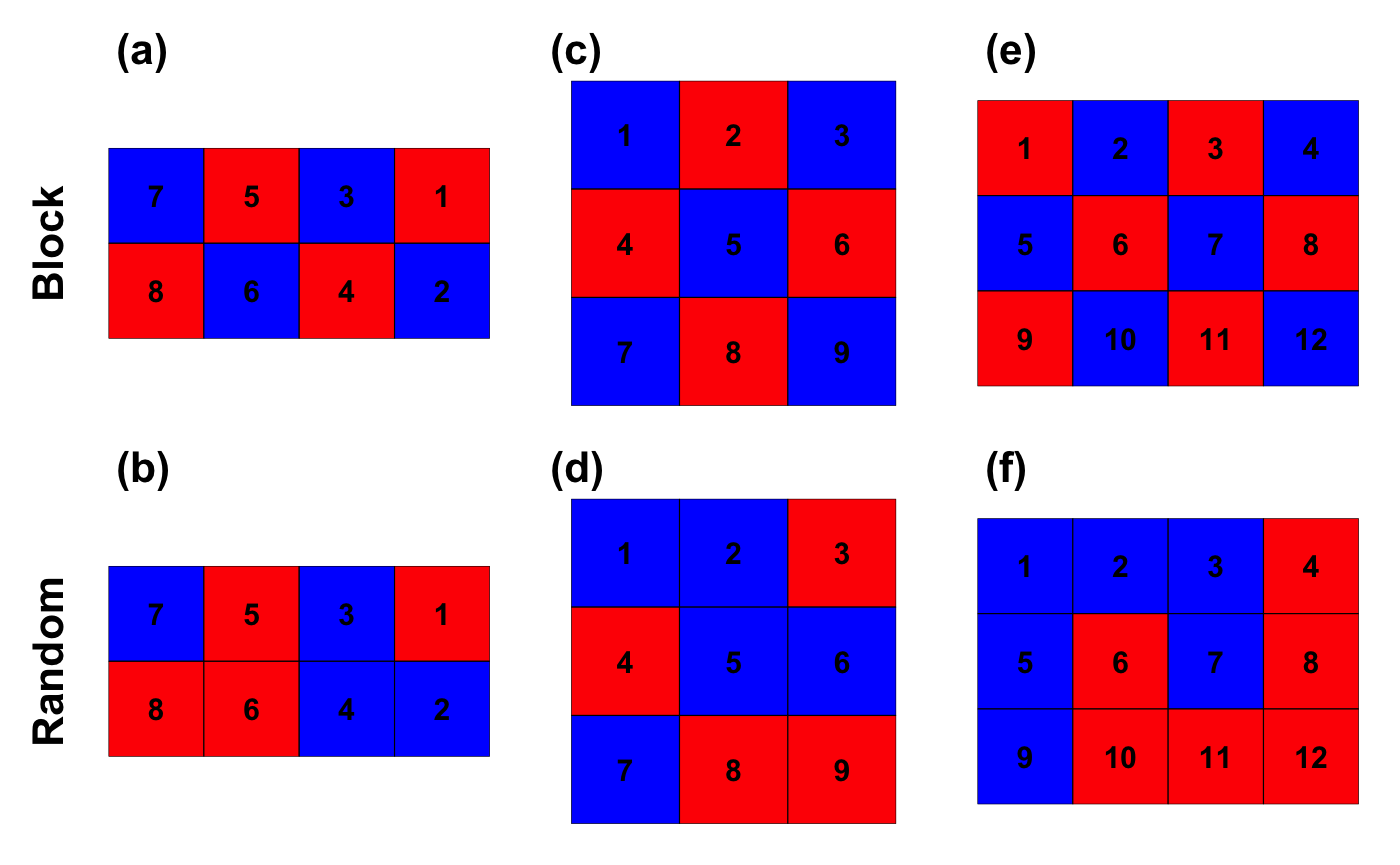
\includegraphics[width=1.0\textwidth]{figures/SpatialGridSetups/GridsCombined.png}
\caption{\DIFaddFL{2x4 (left), 3x3 (middle), and 3x4 (right) spatial grids of intervention (red) and control (blue) clusters assigned via Block Stratified Sampling (top row) and Random Sampling (bottom row)}}
\label{figure:GridsCombined}
\end{figure}

\DIFadd{The salient feature is that BSS collapses an allocation space of 70--924 arrangements down to just 2--6. For the even-celled 2$\times$4 and 3$\times$4 grids this forces an exact checkerboard; on the 3$\times$4 grid in particular every intervention cluster is then surrounded entirely by control neighbors, a structural property that proves consequential under bidirectional spillover (Section~\ref{section:Results}). This drastic reduction is the source of both BSS's principal strength---near-zero variance across its handful of allocations---and its principal limitation: a near-deterministic design that cannot support randomization-based inference (Section~\ref{section:Results}, Section~\ref{section:Limitations}).
}

\subsection{\DIFadd{Spatial Autoregressive (SAR) Model}}\label{section:SAR}

\DIFadd{Outcomes in the presence of spatial dependence and spillover effects can be considered via modeling with a spatial autoregressive}\\ \DIFadd{model\mbox{%DIFAUXCMD
\cite{waller_applied_2004}}\hskip0pt%DIFAUXCMD
\mbox{%DIFAUXCMD
\cite{fotheringham_sage_2009}}\hskip0pt%DIFAUXCMD
\mbox{%DIFAUXCMD
\cite{ullah_handbook_1998}}\hskip0pt%DIFAUXCMD
. A spatial autoregressive model has the form:
}

\begin{equation}\DIFadd{\label{Equation:SARmodel}
    y_{ik} = \rho\sum_{j \neq i} w_{ij}y_{jk'} + \mathbf{x}_i \beta + \varepsilon_{ik}
}\end{equation}

\noindent \DIFadd{where $w_{ij}$ are elements of the row-normalized spatial weights matrix $\mathbf{W}$ (equal to $1 / |\mathcal{N}(i)|$ if clusters $i$ and $j$ share a Rook edge, and 0 otherwise; full construction in Appendix~\ref{appendix:SpatialWeights}); $i$ indexes clusters ($i = 1, \ldots, n$) and $k$ indexes individual subjects within cluster $i$, so the subscripts in $w_{ij}y_{jk'}$ denote cluster $j$ and an individual subject $k'$ in that cluster; $\rho$ is the spatial correlation (autoregressive) coefficient; and $\varepsilon_{ik}$ represents an i.i.d. error term for subject $k$ in cluster $i$. The matrix $\mathbf{W}$ is a cluster-level $n \times n$ adjacency matrix---the subscripts $i$ and $j$ in $w_{ij}$ refer to clusters, not individuals. This can also be expressed in matrix notation as:
}

\begin{equation}
    \DIFadd{\mathbf{y} = \rho\mathbf{Wy}+\mathbf{X}\beta + \varepsilon
}\end{equation}
\DIFadd{It follows that the general form of the response for this model for the purpose of this study is
}\begin{equation}
    \DIFadd{y_{ik} = \alpha + \beta x_i + \psi z_i + \rho\sum_{j \neq i} w_{ij} y_{jk'} + \epsilon_{ik}
}\end{equation}
\DIFadd{where $y_{ik}$ is the response for individual $k$ in cluster $i$; $\alpha$ is the baseline effect; $\beta$ is the }\textit{\DIFadd{direct}} \DIFadd{intervention effect; $x_i \in \{0,1\}$ is the cluster-level treatment indicator (1 if cluster $i$ receives the intervention, shared by all subjects $k$ within that cluster); $\psi$ is the scalar spillover effect parameter; $z_i \in \{0,1\}$ is the cluster-level spillover indicator (1 if cluster $i$ is a Rook neighbor of at least one treated cluster and the spillover type permits it; 0 otherwise); and the spatial lag $\rho\sum_{j \neq i} w_{ij} y_{jk'}$ captures background spatial dependence through the weighted average of neighboring cluster outcomes (equivalently $\rho\mathbf{Wy}$ in matrix form). Because $x_i$ and $z_i$ are cluster-level quantities constant for all subjects within cluster $i$, all individuals in a cluster share the same expected outcome given their cluster assignment; individual responses differ only through the error term $\epsilon_{ik}$. The spatial lag is built from $\rho$, the spatial autocorrelation parameter; $\mathbf{W}$, the row-normalized cluster-level spatial weights matrix (Appendix~\ref{appendix:SpatialWeights}); and $\mathbf{y}$, the full response vector. Finally, $\epsilon_{ik}$ is the i.i.d. error term for subject $k$ in cluster $i$.
}

\DIFadd{It is important to clarify the conceptual distinction between two spatial quantities in this model: the spatial autocorrelation parameter $\rho$ and the spillover effect $\psi$. The parameter $\rho$ is a }\emph{\DIFadd{nuisance}} \DIFadd{parameter reflecting background spatial correlation in outcomes---nearby clusters tend to produce similar outcomes due to shared environmental, demographic, or social factors, independent of any intervention. In contrast, the spillover effect $\psi$ is a }\emph{\DIFadd{causal, design-level}} \DIFadd{quantity representing the indirect effect that an intervention in one cluster exerts on outcomes in neighboring clusters. While both quantities involve spatial proximity, $\rho$ is an intrinsic property of the data-generating process that must be accounted for in order to obtain valid inferences, whereas $\psi$ is of direct scientific interest and often a primary estimand alongside the intervention effect $\beta$. Failure to distinguish these two quantities---or to include both in the model---can produce confounded estimates of the intervention effect. In particular, when spatial dependence is high, failing to include $\rho$ in the model may cause the spillover estimate $\hat{\psi}$ to absorb background correlation, overstating the apparent indirect effect of the intervention.
}

\paragraph{\DIFadd{Estimands and Interpretation.}}
\DIFadd{The quantities $\beta$, $\psi$, and $\rho$ are }\emph{\DIFadd{structural coefficients}} \DIFadd{of the spatial autoregressive model, not marginal potential-outcome contrasts. This distinction matters because the SAR specification in Equation~(\ref{Equation:SARmodel}) places the response on both sides of the equation, so the model's reduced (equilibrium) form is
}\begin{equation}\DIFadd{\label{Equation:ReducedForm}
    \mathbf{y} = (\mathbf{I} - \rho\mathbf{W})^{-1}\left(\alpha\mathbf{1} + \mathbf{X}\beta + \mathbf{Z}\psi + \boldsymbol{\varepsilon}\right).
}\end{equation}
\DIFadd{A change in any cluster's treatment status therefore propagates to all clusters through the spatial multiplier $(\mathbf{I} - \rho\mathbf{W})^{-1}$. As a consequence, a potential-outcome indirect effect such as $E[Y(0,\mathbf{1})] - E[Y(0,\mathbf{0})]$---the contrast between every other cluster being treated versus untreated, holding a focal cluster at control---is a }\emph{\DIFadd{derived}} \DIFadd{quantity that depends jointly on $\beta$, $\psi$, $\rho$, and $\mathbf{W}$, and equals no single coefficient in the model. In particular, when $\rho \neq 0$ even ``control-only'' spillover induces propagation among treated clusters through the multiplier, so $\psi$ should be read as the structural spillover coefficient on $z_i$ rather than as the marginal indirect effect itself. Accordingly, the simulation study that follows evaluates how well each design recovers the }\emph{\DIFadd{structural}} \DIFadd{coefficient $\beta$ used in the data-generating process, and we are careful throughout not to equate $\beta$ or $\psi$ with marginal causal contrasts.
}

\subsection{\DIFadd{Spatial Dependence}}\label{section:SpatialWeightsMatrix}

\DIFadd{Spatial dependence, used interchangeably with spatial autocorrelation, refers to the property of spatial data where observations close to each other tend not be independent of each other. Rather, observations that are close to each other tend to be dependent on each other and influence values of surrounding data. Hence, there is an implied systematic correlation between data at neighboring locations. Spatial correlation can be positive, where similar values tend to be clustered close together, or negative, where dissimilar values are close together. Appropriate consideration of spatial dependence is necessary for performing valid statistical inference as well as for accurate estimation of effects that are modeled. A pair of common methods for assessing spatial autocorrelation are Moran's $\textit{I}$ \mbox{%DIFAUXCMD
\cite{moran_interpretation_1948}}\hskip0pt%DIFAUXCMD
\mbox{%DIFAUXCMD
\cite{moran_notes_1950} }\hskip0pt%DIFAUXCMD
and Geary's $\textit{C}$ \mbox{%DIFAUXCMD
\cite{geary_contiguity_1954}}\hskip0pt%DIFAUXCMD
\mbox{%DIFAUXCMD
\cite{waller_applied_2004}}\hskip0pt%DIFAUXCMD
. Moran's $\textit{I}$ standardizes the spatial auto-covariance by the variance of the data and Geary's $\textit{C}$ utilizes the sum of the squared differences between pairs of data as a measure of co-variation. These test statistics are reliant on the spatial weights matrix. Formal expressions for both statistics are provided in Appendix~D.
}

\DIFadd{The spatial weights matrix $\mathbf{W}$ encodes the strength of spatial connections between observations; its elements $w_{ij}$ can be constructed as indicator-based (Rook contiguity) or distance-based weights, both of which are row-normalized to ensure comparability across observations with differing numbers of neighbors. In this study, row-normalized indicator (Rook contiguity) weights are used throughout. The spatial dependence term of the SAR model is therefore
}

\begin{equation}\DIFadd{\label{Equation:SpatialDepTerm}
    \rho\mathbf{Wy} = \rho\sum_{j \neq i}w_{ij}y_{jk'}
}\end{equation}

\DIFadd{where $j$ indexes clusters, $k'$ indexes a subject in cluster $j$, and $w_{ij} = 0$ whenever clusters $i$ and $j$ are not Rook neighbors, so the sum reduces naturally to neighboring clusters only. Full definitions of indicator-based and distance-based weight construction, including row-normalization formulas, are provided in Appendix~\ref{appendix:SpatialWeights}.
}

\subsection{\DIFadd{Estimation for SAR Model}}

\DIFadd{Maximum likelihood estimation is utilized to gather parameter estimates from the spatial lag model from Section~\ref{section:SAR}\mbox{%DIFAUXCMD
\cite{ord_estimation_1975}}\hskip0pt%DIFAUXCMD
\mbox{%DIFAUXCMD
\cite{bivand_comparing_2015}}\hskip0pt%DIFAUXCMD
\mbox{%DIFAUXCMD
\cite{bivand_computing_2013}}\hskip0pt%DIFAUXCMD
. The subject-level model to be estimated is
}

\begin{equation}\DIFadd{\label{Equation:SARestimation}
    y_{ik} = \rho \sum_{j\neq i}w_{ij}y_{jk'} + \alpha + \beta x_i + \psi z_i + \epsilon_{ik}
}\end{equation}

\DIFadd{where all terms are as defined in Section~\ref{section:SAR}. The full likelihood and log-likelihood expressions, along with details of the MLE derivation, are provided in Appendix~\ref{appendix:SARLikelihood}. In applied tasks, estimates are obtained via the }\texttt{\DIFadd{lagsarlm()}} \DIFadd{function from the }\textbf{\DIFadd{spdep}} \DIFadd{R library\mbox{%DIFAUXCMD
\cite{bivand_r_2022}}\hskip0pt%DIFAUXCMD
.
}

\section{\DIFadd{Simulation Study}}\label{section:Results}

\DIFadd{A simulation study was carried out to consider the contrast of block stratified and random treatment assignment sampling methods with consideration for spillover effects, spatial dependence, and restrictions on spillover application between intervention and control regions. The results of this study are detailed in the remainder of this section.
}

\subsection{\DIFadd{Simulation Scenarios \& Response}}

\DIFadd{We carry out a simulation study to explore how estimation error of the intervention effect in a Spatial CRT varies across a range of spillover effect sizes, the presence or absence of spatial dependence, varying restrictions on clusters where spillover is permitted to occur, and the method of sampling for treatment assignment. Each simulation scenario is composed of a set of these parameters. The baseline effect, $\alpha$, is always assigned as $0.2$. The intervention effect, $\beta$, is always assigned as $1.0$. The spillover effect, $\psi$, has possible values $0.5$, $0.6$, $0.7$, and $0.8$. The spatial dependence parameter, $\rho$ is set as either $0.00$ or $0.01$. The sampling design for each scenario is either Block Stratified Sampling (BSS) or Simple Random Sampling (SRS). Finally, the spillover application type is (1) Control Clusters Only or (2) Control \& Intervention Clusters. Each simulation setting is replicated for each of the spatial grid dimensions discussed previously (2x4, 3x3, and 3x4).
}

\DIFadd{Given that the form of the spatial lag model in Section~\ref{section:SAR} contains the response on both sides of the expression, a separate closed-form expression for data generation must be considered\mbox{%DIFAUXCMD
\cite{fotheringham_sage_2009}}\hskip0pt%DIFAUXCMD
\mbox{%DIFAUXCMD
\cite{baltagi_spatial_2003}}\hskip0pt%DIFAUXCMD
. This data generation expression is
}

\begin{equation}\DIFadd{\label{Equation:DataGen}
    \mathbf{y} = \left(\mathbf{I}-\rho \mathbf{W}\right)^{-1}\left(\boldsymbol\alpha + \mathbf{X}\boldsymbol\beta + \epsilon\right)
}\end{equation}
\DIFadd{where the mean structure is $\alpha + \beta x_i + \psi z_i$, $x_i \in \{0,1\}$ is the cluster-level indicator of whether cluster $i$ receives the intervention, and $z_i \in \{0,1\}$ is the cluster-level indicator of whether cluster $i$ receives any spillover effect; both are shared by all subjects $k$ within cluster $i$.
}

\DIFadd{The estimation model fitted to each simulated dataset is the spatial lag model
}\begin{equation}\DIFadd{\label{Equation:EstModel}
    y_{ik} = \rho\sum_{j \neq i}w_{ij}y_{jk'} + \alpha + \beta x_i + \psi z_i + \epsilon_{ik}
}\end{equation}
\DIFadd{which mirrors the data-generating structure above and is estimated via maximum likelihood using }\texttt{\DIFadd{lagsarlm()}} \DIFadd{(Appendix~\ref{appendix:SARLikelihood}). The fitted model therefore }\emph{\DIFadd{includes}} \DIFadd{the spillover term $\psi z_i$; bias in $\hat{\beta}$ does not arise from deliberately omitting a variable. Rather, it reflects two sources: (1) collinearity between the treatment indicator $x_i$ and the spillover indicator $z_i$, a structural feature of the allocation that varies between SRS and BSS; and (2) the interaction of background autocorrelation $\rho$ with the spatial configuration of treatment assignments.
}

\DIFadd{The first source deserves explicit treatment because it is exact, not merely high, for an entire family of designs. Under block stratified sampling with control-only spillover (TrtNoSpill), the checkerboard allocation places every control cluster adjacent to at least one treated cluster while no treated cluster borders another treated cluster; hence the spillover indicator satisfies $z_i = 1 - x_i$ }\emph{\DIFadd{exactly}} \DIFadd{for all clusters. The design matrix columns for $x_i$ and $z_i$ are then perfectly collinear, so $\beta$ and $\psi$ are not separately identifiable. Writing the mean structure as $\alpha + \beta x_i + \psi z_i = (\alpha + \psi) + (\beta - \psi)x_i$ shows that the intercept absorbs $\psi$ and the treatment coefficient is shifted to $\beta - \psi$; consequently $\hat{\beta}$ estimates $\beta - \psi$ and its bias is $-\psi$. This is precisely the pattern observed in the results: for BSS/TrtNoSpill with $\rho = 0$, the estimated bias of $\hat{\beta}$ is $-0.496$, $-0.597$, $-0.697$, and $-0.798$ at $\psi = 0.5, 0.6, 0.7, 0.8$ respectively (Table~\ref{table:InterventionEstimatesNoSpill}), matching $-\psi$ to within Monte Carlo error. By contrast, most SRS allocations contain at least one control cluster with no treated Rook neighbor (so $z_i = 0$ there), which breaks the exact collinearity and permits partial separation of $\beta$ and $\psi$; this is the structural reason SRS can recover $\beta$ more accurately than BSS in the TrtNoSpill regime. Characterizing how these allocation-induced identification challenges propagate into $\hat{\beta}$ across grid geometries, spillover regimes, and sampling designs is the central aim of this simulation study.
}

\DIFadd{BSS is fundamentally a }\emph{\DIFadd{design-stage}} \DIFadd{tool: the set of valid BSS allocations is determined prior to data collection, and this study evaluates estimator behavior by exhaustively enumerating all possible treatment allocations for each spatial grid. This exhaustive enumeration is feasible for the small grids studied here (70, 126, and 924 total combinations, respectively) and directly characterizes the full design space. The simulation does not claim to support permutation-based frequentist inference under BSS, nor does it use BSS as a basis for a randomization distribution. Rather, model-based inference via SAR maximum likelihood estimation---specifically the }\texttt{\DIFadd{lagsarlm()}} \DIFadd{R function---is the appropriate inferential framework for practitioners implementing either SRS or BSS in an applied study. The role of this simulation is to identify which design choice leads to an estimator with more favorable bias-variance properties when the true data-generating model (SAR with spillover) is correctly specified. An important corollary follows from the small number of valid BSS allocations (2 for the 2$\times$4 grid, 6 for the 3$\times$3 grid, and 2 for the 3$\times$4 grid): if a trialist were to adopt BSS as the randomization mechanism, the allocation would be nearly deterministic, severely limiting the power of any permutation-based randomization test. BSS is therefore best understood as a }\emph{\DIFadd{design-selection criterion}}\DIFadd{---a principled way to identify a spatially favorable allocation prior to data collection---rather than as a randomization distribution suitable for permutation inference. In applied studies, inference should proceed via model-based SAR maximum likelihood estimation regardless of whether SRS or BSS was used for allocation; this constraint is discussed further in Section~\ref{section:Limitations}.
}

\subsection{\DIFadd{Simulation Procedure}}

\DIFadd{The algorithm implemented to perform the simulations for this study is illustrated in the following section. The simulation is performed over all potential cluster treatment combinations (intervention/control) for each of the 2x4, 3x3, and 3x4 cluster spatial grid geometries. The simulation procedure is as follows:
}

\DIFadd{For each spatial grid geometry and simulation scenario, the complete set of possible treatment combinations was enumerated exhaustively (70 for the 2$\times$4 grid, 126 for the 3$\times$3 grid, and 924 for the 3$\times$4 grid). For each combination, $N = 50$ simulation replications were performed for the 2$\times$4 and 3$\times$3 grids and $N = 10$ for the 3$\times$4 grid, with 20 subjects uniformly sampled per cluster in each replication. Outcomes were generated from the SAR closed-form data-generating process (Equation~\ref{Equation:DataGen}), and parameters $(\alpha, \beta, \psi, \rho)$ were estimated via }\texttt{\DIFadd{lagsarlm()}} \DIFadd{for each replication. BSS-valid combinations were identified and tracked separately (2 for the 2$\times$4 grid, 6 for 3$\times$3, and 2 for 3$\times$4). The complete step-by-step algorithm, including BSS identification criteria and aggregation procedures, is provided in Appendix~\ref{appendix:SimAlgorithm}.
}

\DIFadd{Figure~\ref{figure:SampledPoints} presents an example of the 8 cluster 2x4 spatial grid object. 160 subjects (20 subjects for each cluster) with uniformly distributed coordinates are sampled over the area of the spatial object and colored according to their cluster membership. Subject counts are not necessarily identical between any pair of clusters as the sample of subjects is considered over the whole space. Points in any cluster on the grid are subject to the selected treatment (intervention/control) and equally experience any potential spillover along with all other points that are members of that same cluster. We emphasize that the individual within-cluster coordinates serve only to define cluster membership and to visualize the sampled grid; they do }\emph{\DIFadd{not}} \DIFadd{enter the SAR fit. Because $x_i$, $z_i$, and the spatial weights $w_{ij}$ are all defined at the cluster level, the estimator depends on a subject only through the cluster it belongs to, and the simulated point locations within a cluster are not used by the model. Similar illustrative figures of the sampled observations over the spatial grid could be constructed and displayed for the other spatial geometries under consideration in the simulation study.
}

\begin{figure} [!ht]
\centering
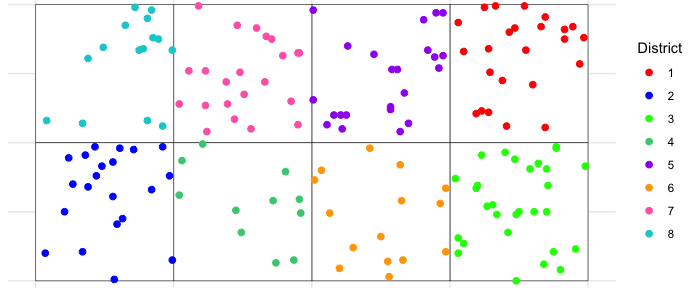
\includegraphics[width=0.80\textwidth]{figures/SpatialGridSetups/SampledPoints.png}
\caption{\DIFaddFL{Example of simulated observation coordinates (n=160) on a 2x4 grid of clusters}}
\label{figure:SampledPoints}
\end{figure}

\subsection{\DIFadd{Simulation Evaluation Metrics}}

\DIFadd{Estimates for the baseline effect ($\alpha$), intervention effect ($\beta$), spillover effect ($\psi$), and spatial correlation parameter ($\rho$) were collected for each iteration of the simulation procedure for every treatment assignment combination. Considering the initial fixed simulation parameters, the following metrics are computed for estimation of the intervention effect for the evaluation of each set of simulation conditions.}\\

\noindent \DIFadd{$\textbf{Bias}$: a measure of how different the estimated parameter value is from the true parameter value. Small bias means that the parameter estimate is quite close to the true value.}\\

\noindent \DIFadd{$\textbf{Variance}$: a measure of the spread of a set of estimates from multiple simulation iterations. Smaller variance indicates that the estimates are tightly grouped together and large variance means that the estimates are spread out.}\\

\noindent \DIFadd{$\textbf{Mean Squared Error (MSE)}$: measures the average squared difference between each estimate and the true value of a parameter. Mean Squared Error combines variance to understand the consistency of a set of estimates as well as bias to understand any trend in deviation from the true value into a measure of estimation accuracy.}\\

\DIFadd{Since $\text{MSE} = \text{Bias}^2 + \text{Variance}$, differences in MSE between SRS and BSS can be attributed to either systematic bias or sampling variability across allocations. This decomposition is visually reflected in the grouped bar figures throughout the Results section (Figures~\ref{figure:BetaMSE2x4Grouped}--\ref{figure:BetaMSE3x4Grouped}), where the relative contribution of bias-driven versus variance-driven error is apparent from differences in bar height across sampling methods and conditions.
}

\DIFadd{Mean Squared Error is the primary metric of consideration to understand the efficient estimation of the intervention effect under all simulation settings. The following subsections detail the findings from the simulation study, focusing on the Mean Squared Error (MSE), standard deviation (SD), and bias of the intervention effect ($\beta$) estimates under various conditions (simulation scenarios). The analysis compares Simple Random Sampling (SRS) and Block Stratified Sampling (BSS) across different spatial grid configurations, spillover effect magnitudes, spatial dependence levels, and spillover application types.
}

\subsection{\DIFadd{Intervention Effect Estimates}}

\DIFadd{We report the Mean Squared Error (MSE), standard deviation (SD), and bias of $\hat{\beta}$ for SRS and BSS across all three grid geometries in Tables~\ref{table:InterventionEstimatesNoSpill} and~\ref{table:InterventionEstimatesSpill}, with the corresponding MSE patterns shown in Figures~\ref{figure:BetaMSE2x4Grouped}--\ref{figure:BetaMSE3x4Grouped}. Rather than narrate each grid in turn, we organize the findings by spillover regime, since the regime---not the grid size---drives the qualitative contrast between the two designs.
}

\paragraph{\DIFadd{Control-only spillover (TrtNoSpill).}} \DIFadd{Here BSS is generally the stronger design, and on the larger grids the advantage is dramatic: for the 3$\times$3 and 3$\times$4 grids BSS attains near-zero MSE with near-zero SD (e.g., BSS MSE $\approx 0.001$ and $\approx 0.0004$ at $\psi = 0.5$, $\rho = 0$, versus SRS MSE $= 0.092$ and $0.034$), because the few checkerboard allocations yield reliably consistent estimates. The 2$\times$4 grid is the lone partial exception: BSS still bounds the worst case (its SD is an order of magnitude smaller than SRS throughout), but when $\rho = 0$ its }\emph{\DIFadd{average}} \DIFadd{MSE can exceed SRS's (BSS $0.262$ vs.\ SRS $0.173$ at $\psi = 0.5$). This is the exact-collinearity regime analyzed in Section~\ref{section:Results}: with $z_i = 1 - x_i$, $\hat{\beta}$ estimates $\beta - \psi$ and carries a bias of $-\psi$---the BSS bias entries of Table~\ref{table:InterventionEstimatesNoSpill} read $-0.496,\,-0.597,\,-0.697,\,-0.798$ for the 2$\times$4 grid at $\rho=0$---so BSS trades a known, design-induced bias for sharply reduced variance.
}

\paragraph{\DIFadd{Bidirectional spillover (TrtSpill).}} \DIFadd{When spillover also flows among treated clusters, SRS is typically the lower-MSE choice on average, though with substantially larger SD: some random allocations carry considerable estimation risk. The important exception is the }\emph{\DIFadd{checkerboard paradox}} \DIFadd{on the 3$\times$4 grid: with spatial dependence present ($\rho = 0.01$), BSS MSE ($\approx 0.223$ at $\psi = 0.5$) substantially exceeds SRS MSE ($= 0.112$), reversing BSS's usual advantage. Because the strict checkerboard surrounds every intervention cluster entirely by control neighbors, bidirectional spillover amplifies rather than dampens the systematic bias in $\hat{\beta}$ (discussed further in Section~\ref{section:Discussion}).
}

\paragraph{\DIFadd{Common patterns.}} \DIFadd{Across all grids and both regimes, increasing the spillover magnitude $\psi$ raises MSE for both designs, and introducing even slight spatial dependence ($\rho = 0.01$) inflates MSE relative to $\rho = 0$. The overarching message is one of risk management: BSS bounds the worst-case estimation error---near-zero SD across its few allocations---and is most advantageous when spillover is confined to control clusters, whereas SRS can achieve a lower average MSE but exposes the analyst to high-variance ``unlucky'' allocations and, under bidirectional spillover with spatial dependence, can outperform a BSS design hampered by the checkerboard paradox.
}

\begin{figure} [!ht]
\centering
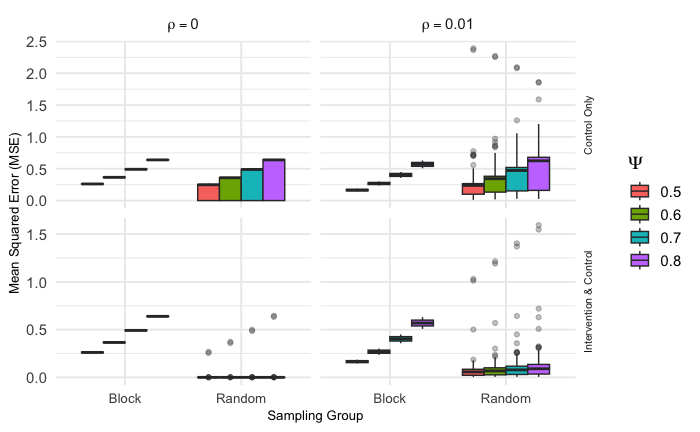
\includegraphics[width=0.80\textwidth]{figures/BetaMSEresults/MSE_Estimates_2x4.png}
\caption{\DIFaddFL{Intervention effect MSE for the 2x4 cluster grid grouped by spillover effect magnitude, spatial dependence, sampling design, and spillover application type.}}
\label{figure:BetaMSE2x4Grouped}
\end{figure}

\begin{figure} [!ht]
\centering
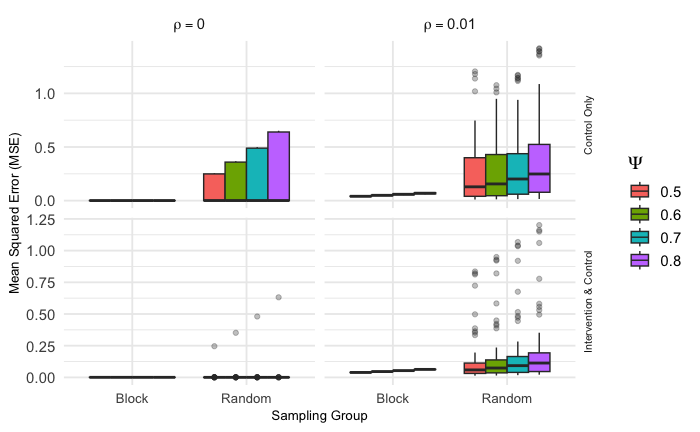
\includegraphics[width=0.80\textwidth]{figures/BetaMSEresults/MSE_Estimates_3x3.png}
\caption{\DIFaddFL{Intervention effect MSE for the 3x3 cluster grid grouped by spillover effect magnitude, spatial dependence, sampling design, and spillover application type.}}
\label{figure:BetaMSE3x3Grouped}
\end{figure}

\begin{figure} [!ht]
\centering
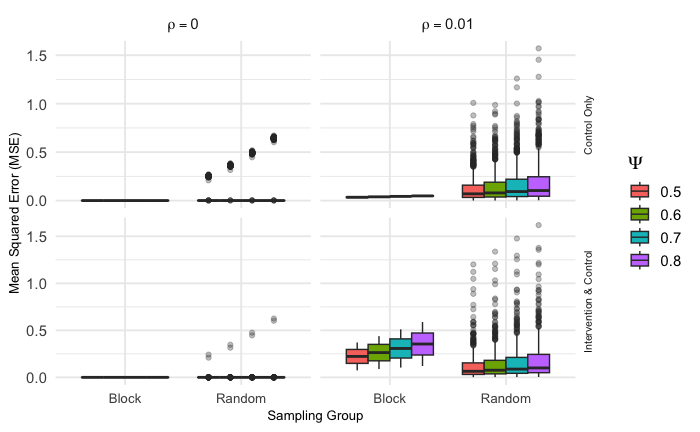
\includegraphics[width=0.80\textwidth]{figures/BetaMSEresults/MSE_Estimates_3x4.png}
\caption{\DIFaddFL{Intervention effect MSE for the 3x4 cluster grid grouped by spillover effect magnitude, spatial dependence, sampling design, and spillover application type.}}
\label{figure:BetaMSE3x4Grouped}
\end{figure}

\begin{table}[ht!]
\centering
{\linespread{1.0}\small\selectfont
\setlength{\tabcolsep}{4.5pt}
\begin{tabular}{l c c ccc ccc}
    \toprule
    \textbf{Grid} & \textbf{\makecell{Spatial \\ Dependence \\ ($\rho$)}} & \textbf{\makecell{Spillover \\ Effect \\ ($\psi$)}} & \multicolumn{3}{c}{\textbf{\makecell{Simple Random\\ Sampling}}} & \multicolumn{3}{c}{\textbf{\makecell{Block Stratified\\ Sampling}}} \\
    \cmidrule(lr){4-6} \cmidrule(lr){7-9}
    & & & MSE & SD & Bias & MSE & SD & Bias \\
    \midrule
    \multirow{8}{*}{\makecell{2$\times$4\\(SD$\times$10)}} & \multirow{4}{*}{\makecell{Yes ($0.01$)}} & 0.5 & 0.304 & 4.053 & -0.270 & 0.165 & 0.294 & -0.349 \\
    & & 0.6 & 0.382 & 4.062 & -0.342 & 0.269 & 0.462 & -0.471 \\
    & & 0.7 & 0.471 & 4.143 & -0.414 & 0.404 & 0.653 & -0.594 \\
    & & 0.8 & 0.573 & 4.390 & -0.486 & 0.569 & 0.867 & -0.716 \\
    \cmidrule(lr){2-9}
    & \multirow{4}{*}{\makecell{No ($0$)}} & 0.5 & 0.173 & 1.170 & -0.343 & 0.262 & 0.095 & -0.496 \\
    & & 0.6 & 0.248 & 1.683 & -0.411 & 0.366 & 0.100 & -0.597 \\
    & & 0.7 & 0.338 & 2.291 & -0.480 & 0.492 & 0.095 & -0.697 \\
    & & 0.8 & 0.441 & 2.994 & -0.548 & 0.639 & 0.081 & -0.798 \\
    \midrule
    \multirow{8}{*}{\makecell{3$\times$3\\(SD$\times$10)}} & \multirow{4}{*}{\makecell{Yes ($0.01$)}} & 0.5 & 0.234 & 2.593 & -0.054 & 0.041 & 0.044 & -0.012 \\
    & & 0.6 & 0.276 & 2.860 & -0.092 & 0.050 & 0.080 & -0.018 \\
    & & 0.7 & 0.322 & 3.284 & -0.131 & 0.059 & 0.114 & -0.022 \\
    & & 0.8 & 0.372 & 3.857 & -0.170 & 0.069 & 0.145 & -0.025 \\
    \cmidrule(lr){2-9}
    & \multirow{4}{*}{\makecell{No ($0$)}} & 0.5 & 0.092 & 1.207 & -0.182 & 0.001 & 0.002 & 0.003 \\
    & & 0.6 & 0.132 & 1.740 & -0.219 & 0.001 & 0.002 & 0.003 \\
    & & 0.7 & 0.180 & 2.370 & -0.255 & 0.001 & 0.002 & 0.003 \\
    & & 0.8 & 0.235 & 3.099 & -0.292 & 0.001 & 0.002 & 0.003 \\
    \midrule
    \multirow{8}{*}{\makecell{3$\times$4\\(SRS SD$\times$100;\\BSS MSE$\times$10,\\BSS SD$\times$100)}} & \multirow{4}{*}{\makecell{Yes ($0.01$)}} & 0.5 & 0.120 & 13.244 & 0.033 & 0.346 & 0.963 & -0.152 \\
    & & 0.6 & 0.138 & 14.807 & 0.021 & 0.388 & 0.505 & -0.167 \\
    & & 0.7 & 0.159 & 17.166 & 0.009 & 0.435 & 0.011 & -0.180 \\
    & & 0.8 & 0.183 & 20.387 & -0.001 & 0.484 & 0.561 & -0.193 \\
    \cmidrule(lr){2-9}
    & \multirow{4}{*}{\makecell{No ($0$)}} & 0.5 & 0.034 & 8.554 & -0.068 & 0.004 & 0.022 & -0.006 \\
    & & 0.6 & 0.049 & 12.318 & -0.081 & 0.004 & 0.022 & -0.006 \\
    & & 0.7 & 0.067 & 16.769 & -0.094 & 0.004 & 0.020 & -0.006 \\
    & & 0.8 & 0.087 & 21.912 & -0.108 & 0.003 & 0.016 & -0.006 \\
    \bottomrule
\end{tabular}}
\caption{\DIFaddFL{SRS vs.\ BSS intervention-effect error estimates ($\hat{\beta}$) under }\emph{\DIFaddFL{control-only}} \DIFaddFL{spillover (TrtNoSpill), for the three grids. Standard deviations (and, for the 3$\times$4 grid, the BSS MSE column) carry the multiplicative factor noted beside each grid; other entries are unscaled. The 2$\times$4 block at $\rho=0$ shows the exact-collinearity signature, with BSS bias $=-\psi$.}}
\label{table:InterventionEstimatesNoSpill}
\end{table}

\begin{table}[ht!]
\centering
{\linespread{1.0}\small\selectfont
\setlength{\tabcolsep}{4.5pt}
\begin{tabular}{l c c ccc ccc}
    \toprule
    \textbf{Grid} & \textbf{\makecell{Spatial \\ Dependence \\ ($\rho$)}} & \textbf{\makecell{Spillover \\ Effect \\ ($\psi$)}} & \multicolumn{3}{c}{\textbf{\makecell{Simple Random\\ Sampling}}} & \multicolumn{3}{c}{\textbf{\makecell{Block Stratified\\ Sampling}}} \\
    \cmidrule(lr){4-6} \cmidrule(lr){7-9}
    & & & MSE & SD & Bias & MSE & SD & Bias \\
    \midrule
    \multirow{8}{*}{\makecell{2$\times$4\\(SD$\times$10)}} & \multirow{4}{*}{\makecell{Yes ($0.01$)}} & 0.5 & 0.095 & 1.762 & 0.031 & 0.165 & 0.294 & -0.349 \\
    & & 0.6 & 0.115 & 2.082 & 0.030 & 0.269 & 0.462 & -0.471 \\
    & & 0.7 & 0.138 & 2.423 & 0.029 & 0.404 & 0.653 & -0.594 \\
    & & 0.8 & 0.162 & 2.787 & 0.027 & 0.569 & 0.867 & -0.716 \\
    \cmidrule(lr){2-9}
    & \multirow{4}{*}{\makecell{No ($0$)}} & 0.5 & 0.008 & 0.438 & -0.014 & 0.262 & 0.095 & -0.496 \\
    & & 0.6 & 0.011 & 0.614 & -0.017 & 0.366 & 0.100 & -0.597 \\
    & & 0.7 & 0.015 & 0.825 & -0.020 & 0.492 & 0.095 & -0.697 \\
    & & 0.8 & 0.019 & 1.072 & -0.023 & 0.639 & 0.081 & -0.798 \\
    \midrule
    \multirow{8}{*}{\makecell{3$\times$3\\(SD$\times$10)}} & \multirow{4}{*}{\makecell{Yes ($0.01$)}} & 0.5 & 0.103 & 1.480 & 0.071 & 0.039 & 0.022 & -0.019 \\
    & & 0.6 & 0.122 & 1.688 & 0.082 & 0.046 & 0.027 & -0.020 \\
    & & 0.7 & 0.143 & 1.905 & 0.092 & 0.054 & 0.032 & -0.021 \\
    & & 0.8 & 0.168 & 2.149 & 0.101 & 0.063 & 0.007 & -0.019 \\
    \cmidrule(lr){2-9}
    & \multirow{4}{*}{\makecell{No ($0$)}} & 0.5 & 0.002 & 0.219 & -0.004 & 0.001 & 0.004 & 0.004 \\
    & & 0.6 & 0.003 & 0.313 & -0.004 & 0.001 & 0.004 & 0.004 \\
    & & 0.7 & 0.004 & 0.428 & -0.005 & 0.001 & 0.004 & 0.004 \\
    & & 0.8 & 0.005 & 0.562 & -0.006 & 0.001 & 0.004 & 0.004 \\
    \midrule
    \multirow{8}{*}{\makecell{3$\times$4\\(SRS SD$\times$100;\\BSS MSE$\times$10,\\BSS SD$\times$100)}} & \multirow{4}{*}{\makecell{Yes ($0.01$)}} & 0.5 & 0.112 & 12.873 & 0.022 & 2.229 & 20.995 & -0.415 \\
    & & 0.6 & 0.131 & 14.762 & 0.021 & 2.634 & 24.750 & -0.452 \\
    & & 0.7 & 0.151 & 16.817 & 0.020 & 3.074 & 28.774 & -0.488 \\
    & & 0.8 & 0.173 & 19.046 & 0.018 & 3.548 & 33.060 & -0.525 \\
    \cmidrule(lr){2-9}
    & \multirow{4}{*}{\makecell{No ($0$)}} & 0.5 & 0.001 & 1.051 & -0.001 & 0.003 & 0.004 & -0.003 \\
    & & 0.6 & 0.001 & 1.542 & -0.001 & 0.003 & 0.004 & -0.002 \\
    & & 0.7 & 0.001 & 2.143 & -0.002 & 0.003 & 0.005 & -0.002 \\
    & & 0.8 & 0.002 & 2.853 & -0.002 & 0.003 & 0.005 & -0.002 \\
    \bottomrule
\end{tabular}}
\caption{\DIFaddFL{SRS vs.\ BSS intervention-effect error estimates ($\hat{\beta}$) under }\emph{\DIFaddFL{bidirectional}} \DIFaddFL{spillover (TrtSpill), for the three grids. Scaling factors are as noted beside each grid. The 3$\times$4 grid at $\rho=0.01$ illustrates the checkerboard paradox, where BSS MSE exceeds SRS.}}
\label{table:InterventionEstimatesSpill}
\end{table}

\section{\DIFadd{Supporting Methods: Spatial-Dependence Diagnostics and Distance-Based Neighbors}}\DIFaddend \label{appendix:MoransI}
%DIF <  (SUPP-4: moved from Section 2.6)
%DIF <  =============================================================================

Before fitting a spatial model, it is advisable to test for the presence of spatial autocorrelation. Two widely used diagnostics are Moran's $\textit{I}$\cite{moran_interpretation_1948}\cite{moran_notes_1950} and Geary's $\textit{C}$\cite{geary_contiguity_1954}\cite{waller_applied_2004}.

\subsection*{Moran's \textit{I}}

Moran's $\textit{I}$ standardizes the spatial auto-covariance by the variance of the data:
\begin{equation}
    \textit{I} = \frac{N \displaystyle\sum_{i}\sum_{j} w_{ij}(x_i - \bar{x})(x_j - \bar{x})}{\left(\displaystyle\sum_{i}\sum_{j} w_{ij}\right)\displaystyle\sum_{i}(x_i - \bar{x})^2}
\end{equation}
where $N$ is the number of spatial units, $x_i$ is the value at location $i$, $\bar{x}$ is the global mean, and $w_{ij}$ are elements of the spatial weights matrix. Values range from $-1$ (perfect negative autocorrelation) to $+1$ (perfect positive autocorrelation); the expected value under the null hypothesis of no spatial autocorrelation is $E[\textit{I}] = -(N-1)^{-1}$. Moran's $\textit{I}$ can be computed in R via \texttt{moran.test()} from \textbf{spdep}\cite{bivand_comparing_2018}.

\subsection*{Geary's \textit{C}}

Geary's $\textit{C}$ uses the sum of squared differences between adjacent observations:
\begin{equation}
    \textit{C} = \frac{(N-1)\displaystyle\sum_{i}\sum_{j} w_{ij}(x_i - x_j)^2}{2\left(\displaystyle\sum_{i}\sum_{j} w_{ij}\right)\displaystyle\sum_{i}(x_i - \bar{x})^2}
\end{equation}
where all terms are as defined above. Values significantly below 1 indicate positive spatial autocorrelation; values above 1 indicate negative autocorrelation; and $E[\textit{C}] = 1$ under the null hypothesis. Geary's $\textit{C}$ can be computed in R via \texttt{geary.test()} from \textbf{spdep}\cite{bivand_comparing_2018}.

%DIF <  =============================================================================
\DIFdelbegin \section{\DIFdel{Distance-Based Neighbor Construction}}%DIFAUXCMD
\addtocounter{section}{-1}%DIFAUXCMD
\DIFdelend \DIFaddbegin \subsection*{\DIFadd{Distance-Based Neighbor Construction}}\DIFaddend \label{appendix:DistanceBased}
%DIF <  (SUPP-5: moved from Section 2.2.2)
%DIF <  =============================================================================

Distance-based neighbors\cite{fotheringham_sage_2009} are constructed under the assumption that clusters within a specified distance of a reference cluster are considered neighbors. As illustrated in Figure~\ref{figure:NeighborPlots}~(c), the reference cell (dark) claims as neighbors all cells whose centroids lie within a specified radius $d_{\max}$. \DIFdelbegin %DIFDELCMD < 

%DIFDELCMD < %%%
\DIFdelend Formally, cluster $j$ is a distance-based neighbor of cluster $i$ if \DIFdelbegin \begin{displaymath}
    \DIFdel{d_{ij} < d_{\max}
}\end{displaymath}%DIFAUXCMD
\DIFdelend \DIFaddbegin \DIFadd{$d_{ij} < d_{\max}$, }\DIFaddend where $d_{ij}$ is the Euclidean distance between the centroids of clusters $i$ and $j$. Distance-based neighborhoods can also be defined for individual point observations rather than areal units; in that case, any point within $d_{\max}$ of the reference point is a neighbor. This definition generalizes Rook contiguity in the sense that, for a regular grid with appropriately chosen $d_{\max}$, the distance-based neighbors coincide with the Rook neighbors (or Queen neighbors if $d_{\max}$ is slightly larger). For irregular geographies, distance-based neighbors offer a flexible alternative that does not require shared boundaries. The corresponding distance-based spatial weights and their row normalization are given in Appendix~\ref{appendix:SpatialWeights}.

\end{document}
